\documentclass[11pt]{svmono}
\usepackage{geometry}        
   
\usepackage[parfill]{parskip}  
\usepackage{graphicx}
\usepackage{amssymb}
\usepackage{epstopdf}
\usepackage{appendix}
\DeclareGraphicsRule{.tif}{png}{.png}{`convert #1 `dirname #1`/`basename #1 .tif`.png}

\usepackage[colorlinks=true, pdfstartview=FitV, linkcolor=blue, 
            citecolor=blue, urlcolor=blue]{hyperref}

%\includeonly{Chapter1}
\usepackage{geometry}                		% See geometry.pdf to learn the layout options. There are lots.
\geometry{letterpaper}    
\usepackage{graphicx}
  \usepackage{amsmath}
 
  \usepackage{tikz}
  \usetikzlibrary{calc,trees,positioning,arrows,fit,shapes,calc}

 \usepackage{tcolorbox}
 \tcbuselibrary{skins}
 \tcbuselibrary{theorems}
\usepackage{hyperref}   
\usepackage{color}
\newcommand{\VAR}{CTRL-r }
\usepackage{xcolor}
         		% ... or a4paper or a5paper or ... 
%\geometry{landscape}                		% Activate for for rotated page geometry
%\usepackage[parfill]{parskip}    		% Activate to begin paragraphs with an empty line rather than an indent
\usepackage{graphicx}				% Use pdf, png, jpg, or eps§ with pdflatex; use eps in DVI mode
								% TeX will automatically convert eps --> pdf in pdflatex		
\usepackage{amssymb}
\usepackage{epigraph}								% TeX will automatically convert eps --> pdf in pdflatex		
\usepackage{proof}
\definecolor{myblue}{RGB}{243,255,255}
\definecolor{mypink}{RGB}{251,229,226}
\definecolor{myyellow}{RGB}{255,255,227}


%\author{The Author}
%\date{}							% Activate to display a given date or no date
%\newcommand{\inp}[1]{\texttt{\colorbox{yellow!25}{#1}}}
\newcommand{\inp}[1]{\begin{tcolorbox}[colback=myyellow,colframe=gray]\texttt{#1} \end{tcolorbox}}

%\newcommand{\proc}[1]{\texttt{\colorbox{green!25}{#1}}}
\newcommand{\proc}[1]{\begin{tcolorbox}[colback=green!35!white,colframe=black]#1 \end{tcolorbox}}

 \newcommand{\coq}[2]{\begin{tcolorbox}[enhanced,title=Goal,coltitle=black, colframe=gray,
          attach boxed title to top left={yshift=-2mm}, colbacktitle=gray!15,bicolor,righthand width=\linewidth/4,colback=myblue, ,colbacklower=mypink ]$#1$ \tcblower
$ #2 \ $ \end{tcolorbox}}

 \newcommand{\coqtwo}[3]{
 \begin{tcolorbox}[bicolor,righthand width=\linewidth/4,sidebyside,colback=green!35!white,colbacklower=gray!10!white] {\small \texttt{#1}}\tcblower
]{\begin{tcolorbox}[bicolor,righthand width=\linewidth/4,colback=gray!10!white,colframe=black, ,colbacklower=orange ]$#2$ \tcblower
$ #3 \ $ \end{tcolorbox}}  \end{tcolorbox}}

 \newcommand{\rmk}[1]{
\begin{tcolorbox}[fonttitle=\bfseries,coltitle=black, title= Remark, colbacktitle=gray!15, colback=gray!5!white,colframe=gray]
#1\end{tcolorbox}}

\newcommand{\warn}[1]{\begin{tcolorbox}[fonttitle=\bfseries,coltitle=black,colframe=red!90, title=!Warning!]#1 \end{tcolorbox}}

\newcommand{\inv}{\mbox{{ \vspace{-3pt} \string^}\!-1}}
\newcommand{\mess}[1]{\begin{tcolorbox}[colback=white,colframe=gray] #1 \end{tcolorbox}}
\newcommand{\code}[1]{\begin{verbatim} #1 \end{verbatim}}

\newtheorem{Theorem}{Theorem}
\newtheorem{Lemma}{Lemma}
\newtheorem{Proposition}{Proposition}
\newtheorem{Definition}{Definition}
\newtheorem{Axiom}{Axiom}
\tcbuselibrary{breakable}


%\newtheorem{theorem}{Theorem}
%\newtheorem{corollary}[theorem]{Corollary}
%\newtheorem{definition}{Definition}
%\newtheorem{lemma}{Lemma}
%\newtheorem{exercise}{Exercise}
%\newtheorem{remark}{Remark}
%\newtheorem{example}{Example}
%\newtheorem{warning}{Warning}
\usepackage{subfiles}
\def\grad{ \mbox{grad}}
\def\curl{ \mbox{curl}}
\def\div{ \mbox{div}}
\def\U{\ensuremath {\cal U}}
\def\S{\ensuremath {\cal S}}
\def\V{\ensuremath {\cal V}}
\def\R{\ensuremath {\cal R}}
\def\tr{\ensuremath {\mbox{tr}}}




% ------------------- Title and Author -----------------------------
\title{Discrete Mathematics with Proof assistants}
\author{Corneliu Hoffman}
\begin{document}


\frontmatter
\maketitle

\tableofcontents

 \frontmatter
\mainmatter

  \preface
\epigraph{Proofs are to mathematics what spelling (or even calligraphy) is to poetry. Mathematical works do consist of proofs, just as poems do consist of characters.}{Vladimir Arnold}
Section{General introduction}
There are numerous studies about the image of mathematics among professional mathematicians and among the general public. The general public holds the idea that Mathematics is a series of formulas and calculations that are useful but are so complicated that they satisfy the old Arthur C Clarke quote ``Any sufficiently advanced technology is indistinguishable from magic.''.

However similar studies among mathematicians provides a completely different result. Indeed most mathematicians think that the main transferable skill that Mathematics Education brings is not the ability to do the long calculations but the ability to reason correctly and to use abstraction in solving problems.

Therefore, while one should not discard the intrinsic value of effective computational tools, Mathematics is ``about proofs''. Mathematics Education should reflect this. This approach is as old as teaching of Mathematics. Euclid's Elements, probably the oldest textbook in the western world is a collection of proofs and constructions. It has lead the teaching of mathematics for much of last two thousand years. 

However, the teaching of proofs is loosing ground  in the modern Mathematics curriculum. Indeed, for example,  in the UK   Advance level exam from 1957,  7 of the 10 questions involved a small proof. By comparison the 2016 equivalent (C4 AQA test), only 16 out of 75 points were proofs. This in not the place to discuss the many reasons for this development. Nevertheless, the result is that many students start university expecting that mathematics  is a series of cookbook methods and computations. One of the most serious stumbling blocks in University Mathematics is the lack of exposure to proofs.

This text is meant to be an attempt to address this. There are, of course, countless textbooks of the kind so writing yet another standard one would be rather pointless. We will  therefore attempt to be a little non-standard.

In the last few decades computer aided education has come to prominence. Computer Algebra systems such as Maple, Mathematica, Mathlab, Maxima, Sage and so on have permeated the curriculum providing examples, modelling, automated assessment and so on. By comparison, the teaching of proofs and abstractions have seen almost none of these.

Of course computer assisted proofs are almost as old as computers. Already in 1954  Martin Davis encoded Presburger's arithmetic and managed to prove that the sum of even numbers is even. More importantly, a few years later  Newell, Simon and  Shaw wrote  the ``Logic Theorist'', a first order logic solver that managed to prove 38 of the theorems in Russell and Whitehead's  ``Principia Mathematica''. The development of PROLOG in the 70's offered a reasonably simple context to verify first order logic.

Until quite recently thought, proof assistants belonged to the world of Computer Science, more precisely program verification. Very little of the advances in the domain crossed over into mathematics or mathematics education.

In the 80's a plethora of Proof assistants came to prominence. While initially they	 mimicked the standard language of mathematics (see for example Mizar), they soon simplified  their notations for the sake of efficiency. Despite attempts by some developers (such as the decorative mode Isar for Isabelle), most proof assistants are beyond the reach of a beginning mathematics student.


We have made several attempts to teach Mathematics with the help of Isabelle and Coq and they all had only modest success. The syntax proved to be too much for the students. The solution we found was to develop a separate interface for Coq that will separate the student from both the terseness and the automation power of the theorem prover and will provide an accessible and interactive syntax. The resulting product is called Spatchcoq, after the method of ``butterflying '' a chicken prior to cooking. We hope that the wonderful authors of Coq would forgive our little inside joke.

The idea of the book is to teach some topics in discrete mathematics (the standard way of introducing proofs) with the help of Spatchcoq. The reader is encouraged to download the software using the instructions in Appendix~\ref{ch:thesoftware}. 


 We will slowly introduce the software together with basic methods of proofs in Chapter~\ref{chap:Basicproof} give numerous examples. The inpatient reader can skip quickly to Appendix~\ref{ch:tactics} to get short descriptions of the tactics, respectively to Appendix~\ref{ch:examples} to see two detailed examples. You can also find some other examples of proofs at 
 
 \url{https://github.com/corneliuhoffman/spatchcoqocaml/tree/master/examples}
\section{Warning for teachers}\label{subsec:warnings}

Spatchcoq is developed on top of Coq and, by extension, will suffer from some of the difficulties inherent in using Coq (or any other proof assistant). Perhaps one of the most important one is the fact that proof assistants are based on type theory rather than set theory (see Appendix~\ref{chap:setsvstypes} for details). In particular every object in Coq has exactly one type and you need a conversion to move form one to the other. We have tried to keep this under the hood as much as possible and to mimic the usual notations and formulations. 

This creates certain surprising complications. For example, in the number theory chapter, we have decided to work with natural numbers rather than integers (this is mainly so that induction will work as expected). In general this is ok but, because $\mathbb{N}$ is not a ring, subtraction is a delicate beast.  This is because, if $m\le n$ are two natural numbers then $m-n=0$. So, for example a statement like $ (m - n) + n = m$ is only true if $m\ge n$. For example $(2-3)+3=0+3=3$. For this reason we advise to tilt your examples in the number theory section towards addition rather than subtraction. We will try to remind the reader about such issues as we go along. We will use the following format:

\warn{Watch for the complications related to minus.}

We will also use some separate coloured boxes to separate txt. More neutral remarks are going to look like this:
\rmk{This is a remark that should help you understand the paragraph better.}


The text that is related to Spatchcoq will also be separated from usual text. The text that we input in to Spatchcoq will appear in input boxes like this:
\inp{
Lemma ancomm$(P\ Q:Prop):P\lor Q ->Q\lor P.$\\
Assume $(P \lor Q)$ then prove $(Q \lor P)$.\\
Consider cases based on disjunction in hypothesis Hyp.}

The goals that Spatchcoq will return to us will look like this:
\coq{Hyp:not\ (P \land (not\ Q))\\
Hyp0:(((not\ P) \land Q) \lor (P \land (not\ Q)))\\
}{Q}

And the messages that Coq will offer look like this:

\mess{error}


 








\mainmatter

\chapter{Basic proof techniques.}\label{chap:Basicproof}

\epigraph{Contrariwise,' continued Tweedledee, 'if it was so, it might be; and if it were so, it would be; but as it isn't, it ain't. That's logic.}{Lewis Carroll}

\section{Motivational Speeches}

 Lewis Caroll,  Oxford Logician and lecturer, delivers a self-deprecating jibe  through the words of Tweedledee. He understood very well the following  simple fact: Logic is hard and often sounds like complete gobbledygook. Nevertheless, Mathematical Logic plays the role of grammar for Mathematics and I hope that by the end of the chapter the reader will disagree with Tweedledee. This also the first place 
 
 

The English language tends to be more nuanced than mathematical logic. For example consider the following   internet meme\footnote{My son Luca showed it to me.}:

The phrase
``I never said she stole my money.'' has 7 different meanings depending on the emphasis. For example ``{\bf I } never said she stole my money'' means perhaps somebody else said it, ``I never said {\bf she} stole my money'' might mean I said that somebody else stole the money  while ``I never said she stole my {\bf money}.'' might means  she stole something else.

 Mathematical logic is a lot more precise than vernacular language. Every statement has to be either true or false. Nuances have no place in logic. You have to formulate statements offering only one interpretation. You will be introduced to the main concepts in the following	chapters. You will also learn about Spatchcoq at the same time.

\section{Propositional Calculus}
\epigraph{Nothing goes over my head. My reflexes are too fast, I would catch it and I would kill it. }{ Drax the Destroyer.}

Propositions form the the building bricks of Mathematical Logic. Not any statement is a proposition, like bricks, propositions need to be build certain specifications in order to hold the edifice of Mathematics. The specifications are quite direct:
\begin{Definition}
A proposition is a sentence which is either true or false but not both.
\end{Definition}

 In other words Mathematical logic is completely literal. No metaphors or second meanings there. Drax the Destroyer likes propositional logic. 
This seems like an rather pompous definition and it seems rather limiting (and prone to endless jokes in the case of poor Drax) but it is very important for what follows. Here are some examples of propositions:
\begin{itemize}
\item Earth is a planet.
\item $2+2=5$
\item $\forall x \in \mathbb{R}, x^2 \ge 0$
\item Men are mortal.
\end{itemize}
The common language is much richer than mere logic, There are questions, metaphors, hyperbolae, oratorical flourishes and so on. Here are some  examples of sentences that fail to qualify as propositions. 

\begin{itemize}

\item What time is it?
\item  We are better off today than 3 years ago.
\item  All the world?s a stage, and all the men and women merely players.
\item $x+3>5$
\item It will rain tomorrow.
\item In the case of Drax there is also the issue of ``Metaphors are gonna go over his head.''
\end{itemize}

But why should one restrict to such mundane requirements? Is it not true that if your restrict your language to the direct and practical, avoid questions, stylistics and oratorial style and state only facts then the language is made of propositions only? Enter an old friend of the sophists, the paradox.
\paragraph{\bf Of paradoxes }
In Titus 1:12-13, the apostle Paul states:
``One of themselves, even a prophet of their own, said, The Cretians are alway liars [...] This witness is true''.  The Cretan Philosopher  Epimenides, the prophet in Paul's text, is usually credited with the first version of the paradox.   For simplicity we look at a slightly modified version:  ``This statement is a lie''. Cicero \cite{Cic} tells us how to think about it ``If you say that you lie and you speak the truth, you lie. But then you say that you lie and you speak the truth, so you lie.''

A modern  take  on the old story is Pinnochio's paradox. Assume that Pinnochio utters the statement: ``My nose grows!'', what happens? If we observe his nose growing then his words ring true and so his nose should have remained proportional to his face. If we see no change in the size of the nose then his statement must have been false and so, as the story tells, his nose is due for a growth spur ...  

Another variant is attributed to Bertrand Russell:
'' Once upon a time there was a small island with extreme trespassing laws. Everyone caught trespassing was interrogated.  If   found to be truthful the guards  will shoot the intruder and if the intruder is found lying the  hangman awaits  them. A logician caught trespassing happily shouts ``You will hang me!''. Of course, in the logic of this island a trespasser  is either shot or hanged. If they hang him then the statement is truthful and so they should have  shot him. If they shoot him then his statement is not truthful so they should have hanged him. The law appears  inconsistent.
These  self referential paradoxes  lead to Russell type paradoxes (see Subsection~\ref{subs:Constructive vs Classical} and 
 Chapter~\ref{ch:settheory} as well as Appendix~\ref{chap:setsvstypes})


  \subsection{Connectors}
Just like for other mathematical concepts, we build a ``calculus'' for dealing with  propositions. Some form of this date back to Aristotle but logicians  modified them thorough the ages. As with any kind of language, we start with simple forms and combine them into more complicated ones. In fact, as usual in the  pedagogical process,  we start with complicated propositions and break them down into  standard combinations of simple forms. To do so define five connectors (operators) on the set of propositions: and ($\land$), or ($\lor$),  implication ($\rightarrow$),   negation( $\neg$) and  double implication ($\leftrightarrow$) . The first four are  ``binary operators'', they combine two propositions . The last one is a ``unary operation''  much like minus is for numbers. Most of these notions will seem familiar to you, our approach will however be a little bit more formal. The symbols are not independent, one can express some of them using the others.

\paragraph{\bf Conjunction (and)}
If $P$ and $Q$ are two propositions then their conjunction, denoted by $P\land Q$  (read ``P {\bf and} Q'') is a proposition that is only true if both $P$ and $Q$ are true. We can write the Truth table bellow:

$$\begin{array}{|c|c|c|}\hline P & Q & P\land Q \\\hline T & T & T \\\hline T & F & F \\\hline F & T & F \\\hline F & F & F\\ \hline\end{array}$$
here are some examples.

\begin{itemize}
\item ``She is both intelligent and hard working'' can be written as (``She is intelligent'')$\land$(``She is hard working'').
\item $0<4<5$ can be written as $(0<4)\land (4<5)$.
\end{itemize}

\paragraph{\bf Disjunction (or)}
 if $P$ and $Q$ are two propositions then their disjunction, denoted by $P\lor Q$ (read `` P {\bf or} Q'' )is a proposition that is only false if both $P$ and $Q$ are false. That is it is true if either $P$ or $Q$ or both are true.  Note that in SpatchCoq you can enter this by either clicking on the symbol or by typing \textbackslash /.
 
 The corresponding truth table is: 
 $$\begin{array}{|c|c|c|}\hline P & Q & P\lor Q \\\hline T & T & T \\\hline T & F & T \\\hline F & T & T \\\hline F & F & F\\ \hline\end{array}$$
 
 Here are some examples:

\begin{itemize}
\item ``He is either at work or on his way home'' can be written as (``He is  at work'')$\lor$(``He is on his way home'').
\item $0\le 4$ can be  written as $(0<4)\lor (0=4)$ 
\end{itemize}
Note that, unlike in nature language, the connector $\lor$ is not an ``exclusive or''. The proposition $P\lor Q$ is true in the case both $P$ and $Q$ are true.


\paragraph{\bf Implication} If $P$ and $Q$ are two propositions then  $P\rightarrow Q$  (read ``P {\bf implies} Q ''or ``{\bf if} P {\bf then} Q'') is a proposition that is only false if  $P$ is true and $Q$ is false. In other words, we can produce the following truth table':
$$\begin{array}{|c|c|c|}\hline P & Q & P\rightarrow Q \\\hline T & T & T \\\hline T & F & F \\\hline F & T & T \\\hline F & F & T\\ \hline\end{array}$$

\begin{itemize}
\item ``If it rains then you need your umbrella'' can be written as (``It rains'')$\rightarrow$(``you need your umbrella'').

\end{itemize}
This is the most counterintuitive of all connectors. Note that if the proposition $P$ is false then $P\rightarrow Q$ is automatically true regardless of the truth value of $Q$.

\paragraph{\bf Negation}
if $P$ is a proposition then its negation, denoted by $\neg P$  ( read ``{\bf not} P'') is a proposition that is  false if  $P$ is true and true if $P$ is false. Note that in SpatchCoq this can be typed by clicking on the symbol or by writing not.
The truth table is very simple:
$$\begin{array}{|c|c|}\hline P & \neg P\\\hline T & F \\\hline F & T\\ \hline\end{array}$$



\begin{itemize}
\item ``It is not raining'' can be written as $\neg$(`` It rains'').
\item $0\le 4$ can be  written as $\neg (0>4)$ 



\paragraph{\bf Double implication (If and only if)}

If $P$ and $Q$ are propositions then $P\leftrightarrow Q$ (read ``P {\bf  if and only if} Q'') is the same construction as $(P\rightarrow Q) \land (Q\rightarrow P)$. It means that the two propositions have the exact same truth value. The truth table is:

$$\begin{array}{|c|c|c|}\hline P & Q & P\leftrightarrow Q \\\hline T & T & T \\\hline T & F & F \\\hline F & T & F \\\hline F & F & T\\ \hline\end{array}$$


As you saw in the definition of $\leftrightarrow$, the various connectors are not independent. For example note the following truth tables:

$$\begin{array}{|c|c|c|c|c|}\hline P & Q & P\rightarrow Q & \neg P & (\neg P)\lor Q \\ \hline T & T & T &F &T\\\hline T & F & F &F &F \\\hline F & T & T &T &T \\\hline F & F & T &T&T\\ \hline\end{array}$$


$$\begin{array}{|c|c|c|}\hline P & \neg P & \neg (\neg P) \\\hline T & F & T \\\hline F & T & F \\\hline\end{array}$$

$$\begin{array}{|c|c|c|c|c|c|c|}\hline P & Q & \neg P & \neg Q & P\lor Q & \neg ( P \lor Q) & (\neg P)\land \neg Q \\ \hline T & T & F &F & T & F & F \\\hline T & F & F &T & T &F & F \\\hline F & T & T & F & T & F & F \\\hline F & F & T &T&F& T & T\\ \hline\end{array}$$


Two composed propositions that have the exact truth values regardless of the values of their components are called equivalent. In other words the statement $P \rightarrow Q$ is equivalent to $\neg P \lor Q$, the propositiont $P$ is equivalent to  $\neg \neg P$ and  $ \neg ( P \lor Q)$ is equivalent to proposition $(\neg P)\land \neg Q $.

A proposition that is equivalent to the proposition True (i.e one that is True regardless of the value of its components) is called a tautology. For example, if $P$ and $Q$ are equivalent then $(\neg P) \lor Q$ is a tautology. In particular  $$ ( P \lor Q) \lor (\neg P\land \neg Q)$$ is a tautology. 

\subsection{Translation between english and propositional calculus}

Many questions in real life are not immediately expressed as an easy propositional calculus term and, depending on how convoluted the text is, it  might be a challenge to translate it into one.  Here are some rules that will help you recognise the logical connectors.


\paragraph{\bf The conjunction ($q\mathbf{\land}p$)} This usually appears as ``and'' in texts. In other words  ``It rains and it's windy can pe written as ``It rains'' $ \land $ ``it's windy'. Other forms: ``but'',``moreover," ``however'',  ``even though'', ``although'', ``nevertheless''. Some of these seem surprising because the suggest a certain implication. For example the statement ``It is sunny although cold.'' should be interpreted as ``it is sunny'' $\land$
 ``it is cold''. Even more bizarrely, you can rewrite the above as ``It is sunny even if it's cold.'' using the word ``if'' which suggests an implication.
 
 \paragraph{\bf The disjunction \bf$p \mathbf{\lor}q$}You usually find this as ``or'' but this is a tricky one. In Mathematical logic, $\lor$ is an ``inclusive disjunction''. This means that if both $p$ and $q$ are true then so is ``p $\lor$ q''. In colloquial English ``or'' might mean exclusive disjunction, that is the statement is true only if exactly one of the components holds true. Often this appears in the ``either ... or ...'' syntagm. Moreover ``unless'' sometimes apears as an $\lor$ replacement and some other times as an exclusive disjunction. The translation of or is much more context dependent.  Drax the Destroyer really dislikes this.
 
 \paragraph{\bf The implication $p \rightarrow q$} is the most complicated connector, its' normal form is  "if ... then ..."  But it can also appear as , "p implies q", "p therefore q", "p hence q", "q if p", "q provided p",  "p is the sufficient for q", and "q is the necessary for  p" or "q follows from p". Perhaps the most difficult to understand for is ``p only if q'' as it seems to be saying $q\rightarrow q$ when in fact it says $p\rightarrow q$.
 
\paragraph{\bf The negation $\neg p$} is a bit more standard, the expression is usually $not p$. Not however the more complex forms of ``neither  p nor q '' meaning ``not p $\land$ not q'' or ``not both b and q are true'' which means ``not (p $\land$ q)'' while ``p and q are both not true '' which means ``not p $\land$ not q''.


\paragraph{\bf The double implication $p \leftrightarrow q$} This usually appears as ``p if and only if q'' or ``p is equivalent to q'' or ``p is necessary and sufficient for q''.

 Let us try to apply our newfound understanding. Consider the statement ``if it;'s Tuesday then I have Maths but not English.'' We have 3 propositions here p:``It is Tuesday.'', q:``I have Maths.'' and r:``I have English. ''. The statement can be written as $p\rightarrow (q \land \neg\ r)$.
 
 
 
 
 
 
\subsection{Inference rules}\label{subset:inference}


Of course any argument in propositional logic can be solved with a truth table. However this is quite tedious and hard to extend to more general notions. We prefer to use methods of proof called "inference rules".
Each connector has two rules, an introduction and an elimination rule. We will also describe them using the standard logic notation. More precisely, the notation
$$\infer[name]{Q}{P}$$
means that the inference rule ``name'' allows you to infer Q from P.



 
\rmk{
In brief, the introduction rule of a connector tells you what to do in order to prove a propositions involving the connector.}
 
\rmk{
The elimination rule of a connector tells you how to use a hypothesis involving the connector to prove other things.
 }

 We will list these in the next section. Note that those connectors will be used later in Predicate calculus and there we will be able to give many more examples. We will also take this opportunity to introduce some of SpatchCoq's tactics.

\paragraph{\bf Forward proofs, backward proofs and implication rules}

Let us describe the {\bf implication introduction rule}.  In order to prove the statement $P\rightarrow Q$ we  assume $P$ and try to prove $Q$. In usual logic notation we have:

$$\infer{P\rightarrow Q}{%
    \infer*{Q}{P}
}$$

The equivalent SpatchCoq tactic is ``Assume P then prove Q.''


The {\bf implication elimination rule} is sometimes called ``modus ponens''. If you have the hypothesis $H:P\rightarrow Q$ and the hypothesis $H1:P$ then you can show $Q$. In logical notation

$$\infer{Q}{P\rightarrow Q & P}$$

In SpatchCoq we use the tactic ``Apply result (H H1)'' or ``Apply result H1.'' followed by ``Apply result H.''



Most of the proofs you have seen written in textbooks are written in a style called ``direct proof''. Suppose you have a set of hypotheses and you want to prove a conclusion. You then start from the hypotheses and prove a series of intermediate results that then get added to you hypotheses until you can prove the conclusion. Most of the time in practice however the way you arrive to a proof is  combining that method with another method called ``backward proof''. 

To fix the details we will prove one example, the famous Aristotelian syllogism:

Socrates is a Man.

All men are mortal.

Therefore Socrates is mortal.

We will be somewhat abusive using 3 propositions {\bf Socrates, Man, Mortal}. We will redo this more carefully in Section~\ref{sec:predicatecalculus}.

We have two Axioms, 
$$\mbox{A1 :  \bf Socrates} \rightarrow \mbox{\bf Man}.$$
$$\mbox{A2: \bf  Man} \rightarrow \mbox{\bf Mortal}.$$



And we need to show that $$\mbox{\bf Socrates} \rightarrow \mbox{\bf Mortal}.$$



To do that we need to use Implication introduction, that is we need to assume {\bf Socrates} and try to prove {\bf Mortal}. 

 We start by giving a ``foward proof'' of this. Since we know  A1 and {\bf Socrates}, implication elimination tells us that we have {\bf Man}. Similarly since we know A2 and {\bf Man}, implication elimination gives you {\bf Mortal}, which is what we needed to prove.

We could have argued backwardly as follows: Since we know A2, by implication elimination, in order to prove {\bf Mortal} it is enough to prove {\bf Man}. Similarly from A1 in order to prove {\bf Man} it is enough to prove {\bf Socrates} which we already have as a hypothesis.

In more complicated proofs one often combines the two methods.

Now start Spatchcoq and continue your exploration of Propositional logic using it.

The corresponding argument in SpatchCoq goes as follows. Sset up the three variables:

\inp{Variables Socrates Man Mortal :Prop.}

Note the format: 

Variables $x_{1} x_{2} \cdots x_{n}$ : Prop.

This means the we name these variables and we declare them to be of  {\bf type} Prop. For more discussions about types see \ref{chap:setsvstypes}.
 
 

And then list the two axioms

\inp{Axiom A1 :  Socrates -> Man.}
\inp{Axiom A2 : Man -> Mortal.}


Note the similarity between axioms and variables. See \ref{chap:setsvstypes} for details.

Note the format 

And finally type
\inp{Lemma soc: Socrates->Mortal.}

This time the effect on Spatchcoq si a bit different. For the first time you get to prove something. More precisely the goals window becomes

\coq{ }{Socrates \rightarrow Mortal}

Click on  that statement to get a hint. Pick the first Hint:

\inp{Assume Socrates then prove Mortal.}

This ``tactic'' modifies the goal:

\coq{Hyp:Socrates}{Mortal}

We can now go two ways. 

The first one is a ``forward proof'', very much like the text above, use:

\inp{Obtain Man applying A1 to Hyp.}
to get
\coq{Hyp:Socrates\\ H:Man}{Mortal}
and then 
\inp{Obtain Mortal applying A2 to H.}
and \inp{This follows from assumptions.}
to finish the proof.

The second method is a ``backward proof'', this is a method preferred by Coq and therefore by SpatchCoq.
\begin{proof}\label{backward Socrates}
 
 \inp{Apply result A2.}
 
 to get
\coq{Hyp:Socrates}{Man}

This is equivalent to the above. What we mean is that using A2, we now only need to show Man.

Now we do
 \inp{Apply result A1.}
 
 to get
 
 \coq{Hyp:Socrates}{Socrates}
 which follows by assumption, that is
 \inp{This follows from assumptions.}
 
 \end{proof}
 Of course this is such a simple example that one can do directly 
 \inp{Apply result (A2 (A1 Hyp)).}
 
Congratulations! You have finished your first proof with SpatchCoq. 
 
 
\begin{tcolorbox}[colback=red!5!white,colframe=black]
This might be the place to notice that implication elimination behaves much like a function application in standard mathematics. If you know $H:P\rightarrow Q$  and you know $H1:P$ then $(H H1)$ is a proof for Q. 

Moreover, the labels of the hypotheses are not mere labels. They are objects of the same type as the respective hypothesis. They can be viewed as witnesses for the truth of the respective propositions. Moreover, if we finish our proof with Qed then the name of Lemma itself becomes a witness for its proof.

 
 \end{tcolorbox}
Indeed try
\inp{Lemma soc: Socrates->Mortal.\\
Assume Socrates then prove Mortal.\\
Apply result (A2 (A1 Hyp)).\\
Qed.\\
Print soc.}

to get 

\texttt{
soc =$ \lambda$ Hyp : Socrates, A2 (A1 Hyp) \\
     : Socrates $\rightarrow$ Mortal}

This tells you  that soc is a function  that takes the witness Hyp of the truth of Socrates and produces a witness A2 (A1 Hyp) of the truth of Mortal.
 We will return to types later.





\paragraph{\bf Inference rules for conjunction}
The conjunction introduction says that in order to prove $P\land Q$, you need to prove both $P$ and $Q$. In logic notation we have
$$\infer{P\land Q}{P & Q}$$
In SpatchCoq the tactic we use is ``Prove the conjunction in the goal by first proving P then Q.''

The Conjunction elimination consists of  two separate rules,
$$\infer{P}{P\land Q} \mbox{and} \infer{Q}{P\land Q}$$ To be more precise, if you know $H:P\land Q$ then you can deduce $H1:P$ and $H2:Q$. The corresponding SpatchCoq tactic is ``Eliminate the conjuction in hypothesis H.''

To exemplify this, we shall prove the commutativity of conjunction.
If $P,Q$ are propositions, then $P\land Q \rightarrow Q \land P$. To do so, we use, as above the implication introduction, so we assume that $P\land Q$ holds and show that $Q\land P$. 

Now we will employ to imply the conjunction elimination. Since we know that $P\land Q$ holds, we also know that $P$ holds and that $Q$ holds. by Conjunction introduction we have that $Q\land P$ holds.

The formal proof in SpatchCoq is a bit more elaborate. We start with the Lemma:
\inp{Lemma ancomm(P Q:Prop) : $P\land Q -> Q \land P$.} 

to get \coq{P Q:Prop}{P\land Q \rightarrow Q \land P}

We then use
\inp{Assume ($P \land Q$) then prove ($Q \land P$).}

to get
\coq{P Q:Prop \\ Hyp : P \land Q}{Q \land P}

We know use
\inp{Eliminate the conjuction in hypothesis Hyp.}
To get
\coq{P Q:Prop \\ Hyp0 : P\\ Hyp1:Q}{Q \land P}

Now we use 

\inp{Prove the conjunction in the goal by first proving Q then P.}

To get two goals
\coq{P Q:Prop \\ Hyp0 : P\\ Hyp1:Q}{Q }

and

\coq{P Q:Prop \\ Hyp0 : P\\ Hyp1:Q}{P}

which can each be solved by

\inp{This follows from assumptions.}





\paragraph{Inference rules for disjunction}

The disjunction introduction consists of two different rules. In order to prove $P\/Q$ you can either prove the left hand side or the right hand side.  tHe logical expressions are
$$\infer[left]{P\lor Q}{P} \mbox{ and } \infer[right]{P\lor Q}{Q}.$$

In SpatchCoq we have thee tactics: ``Prove left hand side.'', ``Prove right hand side.'' and 
``Prove * in the disjunction.''

Disjunction elimination is a bit harder to describe but it is a very natural method of ``case by case'' analysis. If you know $H: P\lor Q$ and you  want to prove $R$ then you need to prove $R$ in case $P$ holds as well as in case $Q$ holds.
$$\infer{R}{P\lor Q &\infer{R}{P} & \infer{R}{Q}}$$

In SpatchCoq the tactic is: ``Consider cases based on disjunction in hypothesis H.''

We now give a detailed proof of the commutativity of disjunction:
$$P\lor Q \rightarrow Q\lor P.$$ 

Of course we first assume $P\lor Q$ happens and show $Q \lor P$. To do so we need to argue by cases using Disjunction elimination.

Case 1: P holds. In this case we will prove the right hand side of the disjunction in the goal.This is an assumption and by disjunction intro we are done.

Case 2: Q holds. In this case we will prove the left hand side of the disjunction in the goal. This is an assumption  and by disjunction intro we are done.

Here is the spatchcoq version

\inp{
Lemma ancomm$(P\ Q:Prop):P\lor Q ->Q\lor P.$\\
Assume $(P \lor Q)$ then prove $(Q \lor P)$.\\
Consider cases based on disjunction in hypothesis Hyp.}

at this point, there are two goals generated.

\coq{P\ Q:Prop\\ Hyp0:P}{P\lor Q}
\coq{P \ Q:Prop\\ Hyp1:Q}{P\lor Q}

These are easily eliminated by

\inp{
Prove right hand side.\\
This follows from assumptions.}
respectively 
\inp{
Prove left hand side.\\
This follows from assumptions.}



\paragraph{Inference rules for negation}

Perhaps this is a little hard to digest at first but the negation of $P$ is the same thing as $P\rightarrow False$. Therefore the inference rules for negation are the same as those for implication. In particular, the negation introduction's logic statement is
$$\infer{\neg P}{\infer{False}{P}}.$$
Therefore th This is an important statement to make and, indeed in SpatchCoq in order to deal with negation you will need to use ``Rewrite goal using the definition of not.'' respectively ``Rewrite hypothesis	H using the definition of not.''. To give an example we shall prove 
$$P \rightarrow \neg \neg P$$
We of course first assume $P$ and then prove $\neg \neg P$. To do this we first note that this is the same thing as $(P->False)->False$ and so we assume $P->False$ and try to show $False$. Since now we know $P->False$ and $P$, we can use implication elimination to get False.




The proof in Spatchcoq is identical:

\inp{Lemma notnot$(P:Prop):P \rightarrow \neg \neg P.$\\
Assume P then prove (not (not P)).\\
Rewrite goal using the definition of not.\\
Assume $(P \rightarrow False)$ then prove False.\\
Apply result (Hyp0 Hyp).}

\end{itemize}

\paragraph{Inference rules for equivalence}

We will not insist here because $P\leftrightarrow Q$ is the same as $P\rightarrow Q \land Q\rightarrow P$ and so the inference rules are derivative. In particular
 in spatchCoq we use  tactic :
 
``Prove both directions of P iff Q.''  

as introduction rule in order to prove $P\leftrightarrow Q$ and the  tactic 


``Eliminate the conjuction in hypothesis Hyp.'' 


to eliminate the hypothesis $Hyp: P\leftrightarrow Q$.



 





\subsection{Constructive vs Classical (proofs by contradiction)}\label{subs:Constructive vs Classical}
\epigraph{I mean, you could claim that anything's real if the only basis for believing in it is that nobody's proved it doesn't exist!} 
{J.K. Rowling}
Classical logic includes a certain axiom that the romans called ``tertium non datur'' or ``the excluded middle''. This Axiom states that of $P$ is a proposition then $P\lor \neg P$ always hold. 

 At the beginning of the 20th century a number of mathematicians started debating the need for such an axiom. They came to be collectively called intuitionists. The trouble with that position was that it took away from the power of this axiom without necessarily offering something in return. The things you are able to prove are much more restrictive. As a consequence classical logic carried the day.

However at the end of the century, as Theoretical Computer Science started to gain strength and depth, excluding the excluded middled carried another promise: computability. Via the Curry-Howard correspondence, a ``constructive proof'' (i.e. one without the rule of excluded middle) is equivalent to the construction of a function. In particular, the familiar ``proof by contradiction'' relies on a variant of the excluded middle, namely the fact that the statements $P$ and $\neg \neg P$ are equivalent. We have seen that $P \leftarrow \neg \neg P$ above but the other implication relies on classical logic.

Some ``constructivists'' argue that a proof of $P$ should be a witness to its truth and not merely to the falsity of its negation (as it is the case with $\neg \neg P$.  The motto from JK Rowling does exactly that. This carries quite a bit of weight in the CS world even if not (yet) so much in the Mathematical world.

One of the main methods of "classical logic" is the so called "proof by contradiction". In brief, if you want to prove $P$ then you assume that $P$ is false and then prove a contradiction. The SpatchCoq tactic 
"Prove by contradiction." will transform the statement

\coq{\cdots}{P}

into 
\coq{\cdots\\ H: \neg P}{False}


As an example of proof by contradiction, consider $P$ a proposition and $\neg \neg P$ its double negation. Are these two statements equivalent? We have proved above one of the implications. The converse, however is a bit stranger and requires a proof by contradiction.

\inp{
Lemma oneway (P:Prop): $\neg \neg P\rightarrow P.$\\
Assume (not (not P)) then prove P.}


at this point we have 

\coq{ P:Prop\\
Hyp:not  (not  P)\\
}{P}

so we will employ 
\inp{
Prove by contradiction.}

to get
\coq{ P:Prop\\
Hyp:not  (not  P)\\
H:not P
}{False}
 The rest is quite standard.
\inp{
Apply result Hyp .\\
This follows from assumptions.}

We are not ready to abandon the path of classicism and will assume excluded middle for now. We would however, try to eliminate needlessly using proofs ``by contradiction''.
This is a good point to look at the axiom "classic". If we apply
\inp{Check classic.}

we get the resulst $$classic
    : \forall  P : Prop, P \lor \neg P$$


Therefore, while not an actual independent tactic, applying

"Apply result classic."
will solve any goal that looks like

$$P \lor \neg P.$$

For example let us prove that 
\inp{Lemma a (P Q:Prop): $(P\rightarrow  Q) \rightarrow (\neg P \lor Q)$.
}

We of course first use implication intros by applyiong
\inp{Assume $(P \rightarrow Q)$ then prove $((\neg P) \lor Q)$.}

and get:

\coq{P Q:Prop\\Hyp: P\rightarrow Q}{\neg P \lor Q}

At which point we are stuck without any obvious new possibility to advance. We note however that if P was true then we could use Hyp to obtain Q and if $\neg P$ is true then we would have the disjunction automatically. Thefore we do

 

\inp{Claim ($P \lor \neg P$).\\
Apply result classic.}

To have
\coq{P Q:Prop\\Hyp: P\rightarrow Q\\ H:P \lor \neg P.}{\neg P \lor Q}



We now do a proof by cases that offers no surprises.



\inp{Consider cases based on disjunction in hypothesis H .
Prove right hand side.\\
Apply result Hyp .\\
This follows from assumptions.\\
Prove left hand side.\\
This follows from assumptions.}


Note that the converse is quite easier only requiring  a proof by contradiction.

\inp{Lemma b $(P Q:Prop): (not P \lor  Q)\rightarrow (P\rightarrow Q).$\\
Assume $((not P) \lor Q)$ then prove$ (P \rightarrow  Q).$\\
Assume P then prove Q.\\
Consider cases based on disjunction in hypothesis Hyp .\\
Prove by contradiction.\\
Apply result Hyp1.\\
This follows from assumptions.\\
This follows from assumptions.}


See \ref{sec:drinker} for a rather surprising example of classical logic.

\subsection{Know thine fallacies}

Consider the usual modus ponens rule. 
\infer{P}{\begin{array}{l}Q\\ P \rightarrow Q \end{array}}

Small variations can make this false.
 Consider for example the following argument from Mounty Python and the Holly Grail.
 
 
 
 \infer{\mbox{ It is Tusday }}{\begin{array}{l}\mbox{If it is Tuesday then I play poker }\\ \mbox{I play poker}\end{array}}
 
 
 
 This is one of the most common "formal" fallacy. It is called "Affirming the consequence". Recall that if $P$ is false then $P\rightarrow Q$ is automatically true if $P$ is false and so the deduction above does not hold. It is, however, remarkably prevalent in public discourse especially in adverx

\subsection{A puzzle}

We will now use a puzzle to give a more serious example	 of propositional calculus, its inference rules and their implementation in SpatchCoq. 

The puzzle, ``the lady or the Tiger'' comes from the book  ``The Lady Or the Tiger?: And Other Logic Puzzles'' by Raymond M. Smullyan. It is slightly adapted for the 21st century.

A  prisoner is offered the choice between two doors. Behind each door he could find either the key to his freedom or a very hungry tiger.

 \begin{itemize}

 \item The clue on the first door reads ``the key to your freedom  is in this room and the tiger in the other''.
 \item The clue on the second door reads ``one of the rooms contains  the key to your freedom and the other room the tiger.''
  \item He knows that one of the two clues is correct and the other is incorrect.
 \end{itemize}

What would you do in his place?

We will formalise the questions as follows: We will denote by P the proposition  ``the first room contains the key to freedom'' and by Q the proposition ``the second room contains the key to freedom''. Of course $\neg P$ means ``the first room contains the tiger'' and  $\neg Q$ means ``the second room contains the tiger''.

The clue on the first door is ``the key to your freedom  is in this room and the tiger in the other'' which can be written as $$D1:P\land \neg Q$$.

The second door clue is ``one of the rooms contains  the key to your freedom and the other room the tiger.'' which can be rewritten as ``{\bf either} the first room has the key and the second the tiger {\bf or} the first room has the tiger and the second the key'' so we can write it as:
 $$D2 : (P\land \neg Q) \lor (\neg P \land Q).$$ 
 
 The fact that exactly one clue is correct and the other is incorrect can be written as ``{\bf either} the first door is correct and the second incorrect {\bf or} the first door is incorrect and the second is correct''. This can be written as $(D1 \land \neg D2 )\lor (\neg D1 \land D2)$ which expands to $$((P\land \neg Q)\land \neg ((P\land \neg Q) \lor (\neg P \land Q)))\lor (\neg(P\land \neg Q) \land ((P\land \neg Q) \lor (\neg P \land Q))).$$ 

This looks horrible. We will however show that the second room has the key, that is Q.


For example, the statement we want to prove is 
$$(D1 \land \neg D2 )\lor (\neg D1 \land D2)\rightarrow Q.$$ 
We can set-up SpatchCoq with

\inp{Variables P Q:Prop.}

to define the two propositions $P$ and $Q$.
Then define 

\inp{Definition D1:= $P \land \neg Q.$}

\inp{Definition  D2:= $( \neg P \land Q)\lor(P \land \neg Q)$.}
\inp{Definition onlyone:= $(D1 \land \neg D2)\lor(\neg D1 \land D2)$.}
\inp{Lemma a: onlyone  $\rightarrow Q.$}

After applying the tactic 
\inp{Assume onlyone then prove Q.} we get

\coq{Hyp: onlyone}{Q}
We now use the tactic that we used for not:
\inp{Rewrite hypothesis Hyp  using the definition of onlyone.}
to get

\coq {Hyp: (D1 \land (not \ D2)) \lor ((not\ D1) \land D2)}{Q}

We now use 
\inp{Consider cases based on disjunction in hypothesis Hyp .}
to get two new goals

\coq {Hyp0:D1 \land (not\ D2)}{Q}

and


\coq {Hyp1:not\ D1 \land  D2}{Q}


\inp{Eliminate the conjuction in hypothesis Hyp0.\\
Rewrite hypothesis Hyp1  using the definition of D2.\\
Rewrite hypothesis Hyp  using the definition of D1.
}

brings us to

\coq{Hyp:(P \land (not\ Q))\\
Hyp1: not\ (((not\ P) \land Q) \lor (P \land (not\ Q)))}{Q}

we will now use the proof by contradiction (see \ref{sec:proofbycontradiction})
\inp{
Prove by contradiction.}

to get

\coq{Hyp:(P \land (not\ Q))\\
Hyp1: not\ (((not\ P) \land Q) \lor (P \land (not\ Q)))\\ H:not\ Q}{False}

We note that Hyp1 is of type (not X) that is (X$\rightarrow$False) and so we can apply it (as in the backward proof mentioned above)

\inp{Apply result Hyp1} 
gives


\coq{Hyp:(P \land (not\ Q))\\
Hyp1: not\ (((not\ P) \land Q) \lor (P \land (not\ Q)))\\
H : not\ Q}{((not\ P) \land Q) \lor (P \land (not\ Q))}

Now we note that Hyp is exactly the right hand side of the disjunction so we can use.

\inp{Prove right hand side.\\
This follows from assumptions.}

to finish up this part of the proof.

we are now left with

\coq {Hyp1:not\ D1 \land  D2}{Q}

and, as above we do
\inp{Eliminate the conjuction in hypothesis Hyp1.\\
Rewrite hypothesis Hyp  using the definition of D1.\\
Rewrite hypothesis Hyp0  using the definition of D2.}

to get:
\coq{Hyp:not\ (P \land (not\ Q))\\
Hyp0:(((not\ P) \land Q) \lor (P \land (not\ Q)))\\
}{Q}

Since Hyp0 is a disjunction we do
\inp{Consider cases based on disjunction in hypothesis Hyp0 .}

To get again a case by case analysis.

\coq{Hyp:not\ (P \land (not\ Q))\\
Hyp1:(not\ P) \land Q\\
}{Q}

and

\coq{Hyp:not\ (P \land (not\ Q))\\
Hyp2:P \land (not\ Q)\\
}{Q}

In the first case we use

\inp{Eliminate the conjuction in hypothesis Hyp1 .\\
This follows from assumptions.}

and in the second we prove by contradiction

\inp{Prove by contradiction.\\
Apply result (Hyp Hyp2).\\
Qed.}
\subsection{On the way to the barbershop }

I'd like to thank Richard Kaye for introducing me to this ``paradox''.  In a paper published in 1894 called ``A logical paradox'' Lewis Carroll presents the following situation:

Two uncles want to go the barbershop. There are three barbers, Allen Brown and Carr. We are told that at least one of them has to be in at all times. Also we know that Allen  ``ever since he had that fever he's been so nervous about going out alone, he always takes Brown with him. '' 

One of the uncles then argues that Carr has to be home. The argument is a proof by contradiction. Suppose that Carr is out.  Then if Allen is out then Brown will have to be in since somebody should be in the shop. On the other hand if Allen is out the Brown will have to be out as well on account of Allen's nervousness. Therefore Carr being out generates two contradictory statements ``if Allen is out then Brown is in'' and ``if Allen is out then Brown is out'' and so Carr must be in.

This is a remarkable statement. It is reasonably easy to see what is wrong in today's terms (we shall write a careful argument in a moment) but  at the end of the 19th century  this was serious stumbling block for logicians. In fact in his 1903 book  ``the Principles of Mathematics'', Bertrand  Russell writes:

{\quote  ``The principle that false propositions imply all propositions solves Lewis Carroll's logical paradox in Mind, N. S. No. 11 (1894). The assertion made in that paradox is that, if p, q, r be propositions, and q implies r, while p implies that q implies not-r, then p must be false, on the supposed ground that q implies r and q implies not-r are incompatible. But in virtue of our definition of negation, if q be false both these implications will hold: the two together, in fact, whatever proposition r may be, are equivalent to not-q. Thus the only inference warranted by Lewis Carroll?s premisses is that if p be true, q must be false, i.e. that p implies not-q; and this is the conclusion, oddly enough, which common sense would have drawn in the particular case which he discusses''.}

Indeed the principle that if $p$ is false then $p\rightarrow q$ is true, as seen in the truth table of the implications  was something that was only formalised by Russell. In fact he states that $p\lor q$ is equivalent to $(p \rightarrow q) \rightarrow q$ (see for example \ref{russel}).

Note that B Russell already suggests the answer to the parable. The two statements only prove that if Carr is out then Allen must be in. Let us prove that ins Spatchcoq.

We will define 3 propositions, Allen, Brown and Carr to mean that the corresponding people are in  and state two axioms, $not Allen->not Brown$ and $Allen \lor Brown \lor Carr$ and we prove that $ not Carr \rightarrow Allen$.

\inp{Variables Allen Brown Carr :Prop.\\
Axiom some: Allen $\lor$ Brown $\lor$ Carr.\\
Axiom AB: not Allen ->not Brown.\\
Lemma A: not Carr -> Allen.}

Now we assume that Carr is out and prove that Allen must be in. We use the axiom some to get $Allen \lor (Brown \lor Carr)$.

\inp{Assume (not Carr) then prove Allen.\\
Claim (Allen $\lor$ Brown $\lor$ Carr).\\
Apply result some.}


We get
\coq{Hyp: not Carr\\
H:Allen \lor Brown \lor Carr}{Allen}
The next step is to consider the two  cases: either Allen is home or one of Brown or Carr must be home. If Allen is home then we are done. 
\inp{Consider cases based on disjunction in hypothesis H .\\
This follows from assumptions.
}


We now have
\coq{Hyp: not Carr\\
Hyp1: Brown \lor Carr}{Allen}


We will prove this by contradiction:
\inp{Prove by contradiction.}

To get
\coq{Hyp: not Carr\\
Hyp1: Brown \lor Carr\\ H:not Allen }{False}


We again consider two cases, either Brown happens or Carr happens. In the first case we use the axiom AB

\inp{Consider cases based on disjunction in hypothesis Hyp1 .\\
Apply result AB.\\
This follows from assumptions.
This follows from assumptions.}
 
We are left with the last case:
 
\coq{Hyp: not Carr\\
Hyp2:  Carr\\ H:not Allen }{False} 

Ans so we can finish by applying  modus ponies

\inp{Apply result (Hyp Hyp2).}
 \paragraph{\bf Exercises}\label{prop:exercises}
 \begin{enumerate}
 
 \item[assume] $P \rightarrow P$.
 \item[left]$ P \rightarrow P\lor Q$.
  \item[distr] $P\land (Q\lor R) \rightarrow P\land Q)\lor (P\land R).$
  \item [contrap]$ (P\rightarrow Q) \rightarrow (\neg Q \rightarrow \neg P)$
  \item[implies] $(P\rightarrow Q)\rightarrow (\neg\,P\,\lor \,Q).$
\item[deMorgan] $\neg\,(P\lor Q)\rightarrow (\neg\,P\,\land \neg\,Q).$

  
 \item[impand] $((P \rightarrow Q) \land (P \rightarrow R)) \leftrightarrow (P \rightarrow (Q\land R))$
\item[impor] $((P \rightarrow Q) \lor (P \rightarrow R)) \leftrightarrow (P \rightarrow (Q\lor R))$
\item[andimp] $(P\rightarrow(Q\rightarrow R)) \leftrightarrow ((P\land Q) \rightarrow R)$.
\item[andorimp] $((P \rightarrow R) \land (Q \rightarrow R)) \leftrightarrow ((P \lor Q) \rightarrow R)$
\item[orandimp] $((P \rightarrow R) \lor (Q \rightarrow R)) \leftrightarrow ((P \land Q) \rightarrow R)$
\item[triplenot] $\neg (\neg (\neg P))  \leftrightarrow \neg P$
\item[twoone] $(P \lor Q) \land \neg  P \rightarrow Q$
\item[twotwo] $\neg Q \land (P \rightarrow Q) \rightarrow  \neg P$
\item[twothree] $ C \land (A \rightarrow B) \land (C \rightarrow ( A \rightarrow \neg B)) \rightarrow \neg A$
\item[twofour] $ (P \lor  Q) \land (\neg P \lor R) \rightarrow Q \lor R$.

\item[Russell] \label{russel} $(P\lor Q)\leftrightarrow ((P\rightarrow Q)\rightarrow Q)$



\end{enumerate}

\section{Predicate calculus}\label{sec:predicatecalculus}

Nice as it might be, propositional calculus is not complete enough to express what we want. Here are some example of statements that we would like to deal with
\begin{itemize}
\item The equation $x^2+x+1=0$ does not have any solution.
\item Some people like bread and some do not.
\item If $a,b, c$ are natural numbers,$a|b \land a | c \rightarrow a | (b+c)$.
\item Any differentiable function is continuous.
\end{itemize}

All these require more general notion than that of a proposition, that of a predicate. 
For example $x>0$ might or might not be true depending on $x$. We can view this as a function from $\mathbb{R}$ to the sett of propositions or as a set of propositions, parametrised by $\mathbb{R}$. 

This exactly the meaning of a predicate, it is a collection of propositions parametrised by a context (type). More precisely a predicate is a function $P: U \rightarrow Prop$. 

Here are some predicates.

\begin{itemize}
\item P(x): $x^{2}+x+1 =0$ (here x is a real number).
\item P(p): p is a prime. (here p is a natural number)
\item P(x) : x is a man. (here x is an animal)
\item P(x, y) : x > y. (here both x an y are real numbers and so P : $mathbb{R}^{2}\rightarrow Prop.$

\end{itemize}	

Of course you cannot really prove predicates, just statements. Predicates have ``free'' variables and those need to be ``quantified''. There are two quantifiers that bind variables. as with connectors for propositions they have introduction and elimination rules.

\subsection{\bf Quantifiers, free and bound variables.}

As mentioned above, a predicate is a function which takes values in Prop. As such it has at least free variable (we might consider several variable. predicates). There are two ways to bind predicates,  the existential and the universal quantifier. You have used both of them in a somewhat informal way.
  Very often you see the following colloquial statements.
  
 " Show that $x^2 > 0$. "
  
  This is formally incorrect and its correct statement is : " Show that for any real number $x, x^2 > 0$.  
The second statement is false since $x=0$ is a counterexample. The first one is not a statement unless $x$ has been defined earlier and, if it has, it might be true or false.

  
  
The  {\bf existential quantifier} is denoted by $\exists$. Its meaning  is quite self explanatory. If $P:U \rightarrow Prop$ is a predicate then $\exists x:U, P(x)$ is a proposition which is true if you can find an x so that $P(x)$ is true. Note that in SpatchCoq you can enter this either by clicking on the symbol or by typing exists.


For example $\exists x:\mathbb{R}, x^{2}+x+1 =0.$ means that the equation $x^{2}+x+1=0$ has a solution. Therefore our first example of the section ``The equation $x^2+x+1=0$ does not have any solution.'' can be written as $\neg (\exists x:\mathbb{R}, x^{2}+x+1 =0).$ 

If we consider the predicate ``P(x) : x likes bread'' on the set People of all people then ``Some people like bread and some do not.'' can be written as $(\exists x:People, P(x))\land (\exists x:People, \neg P(x))$.

The {\bf universal quantifier} is denoted by $\forall$. As with the existential quantifier, the meaning of this is natural, the proposition $\forall a, P(a)$ will hold if  the propositions $P(x)$ will hold no matter what x is. 
Note that in SpatchCoq you can enter this either by clicking on the symbol or by typing forall.

Note that you can encounter this in many forms.  Here are some examples:

"All square integers are non-negative" is the same thing as $\forall x \in \mathbb{Z}, x^2\ge 0$.

"The sum of any two odd numbers is even" is the same thing as $\forall x  \in \mathbb{Z} \forall y \in  \mathbb{Z} ,  odd(x) \land odd(y) \rightarrow even(x+y)$.

"Anybody has a friend" is the same thing as $\forall x, \exists y, friend (x,y)$.

Note that bound variables can be renamed. For example $\forall x, \exists y, friend (x,y)$ is the smae as
$\forall y, \exists x, friend (y,x)$. They are also local variables so they can be reused. for example 
$\forall x, P(x)\rightarrow \exists y, P(y)$ can be also writtnen as $\forall x, P(x)\rightarrow \exists x, P(x)$. However one needs to be careful doing this.

\paragraph{\bf Inference rules}

The {\bf existential introduction} rule: if you have a way to prove $P(a)$ for some $a:U$ then you have proved $\exists x:U, P(x)$. In logic notation this is
$$\infer{\exists x:U, P(x)}{P(a)}.$$

In Spatchcoq the tactic that you need in this case is ``Prove the existential claim is true for a.''. In order to apply this tactic you need the goal to be of the form $\exists x:U, P(x)$ and if you apply it you now need to prove $P(a)$.

Here is a very simple example. Suppose you want to prove that $\exists x, x^2=4$. To do so we note that $2^2=4$ and so by existential introsductio the result is true. The proof in spatchcoq is
\inp{Lemma triv:$\exists n:nat, n^2=4.$\\
Prove the existential claim is true for 2.\\
This follows from reflexivity.}
The  {\bf existential elimination} rule: that if you have a hypothesis of the form $\exists x, P(x)$ then you can deduce $P(a)$ for some a. The logic form is

\infer{P(a) \mbox{ for some a}}{\exists x:U, P(x).}

The corresponding SpatchCoq tactic is ``Fix VAR the existentially quantified variable in VAR.''. More precisely if you have a goal that looks like
\coq{H:\exists x:U, P(x)}{...} then the tactic ``Fix a the existentially quantified variable in H.'' will produce a new goal of the form

\coq{a:U\\
H:P(a)}{...}


The {\bf universal elimination} rule: you know $\forall x, P(x)$ you can deduce $P(a)$ regardless of $a$. The logical notation you is

\infer{P(a) \mbox{ for any a}}{\forall  x:U, P(x).}

The SpatchCoq tactic is a bit harder to explain. If you have

\coq{
H:\forall x:U,  P(x)}{...}
you can use 

"Obtain P(a) using variable a in the universally quantified hypothesis H."

To exemplify this we first consider the following statement

$$\forall x:U, P x \rightarrow \exists x:U, P x.$$

Nothing simpler than that right? If a statement is true for all possible values then is of course true for some value. Except for the case where there are no elements of type $U$ at all. In that case the statement $\forall x:U, P x$ will be true but the statement $\exists x:U, P x$ will be false\footnote{
 Sounds confusing? Does it remind you of another confusing constructor? If you said "implies" then you were right. In fact implies is syntactic sugar  for a special case of forall. More precisely $P\rightarrow Q$ is the same thing as $\forall a:P, Q$, that is for the statement that if you know a proof for $P$ you get one for $Q$. We will not insist here, the interested reader can have a look at \cite{coqdart}}.
 
 To remedy that, we shall assume the the type $U$ is nonempty. Here is a proof of the statement
 \inp{Variable U:Type.\\
Lemma a( a:U)($P: U\rightarrow Prop$): ($\forall x:U, P x)\rightarrow \exists x, P x.$\\
Assume ($\forall  x : U, P x$) then prove ($\exists x : U, P x$).\\
Obtain (P a) using variable a in the universally quantified hypothesis Hyp.\\
Prove the existential claim is true for a.\\
This follows from assumptions.}


 Coq is good at universal elimination and can often match the value of the variable  and so if the statement is something like this

\coq{a:U\\ H:\forall x:U, P x }{P a}

then just using 

Apply result H.

 finishes the proof. For example the proof above can be done as follows:

\inp{Variable U:Type.\\
Lemma a( a:U)(P: U->Prop): $(\forall x:U, P x)\rightarrow \exists x, P x$.\\
Assume ($\forall  x : U, P x$) then prove ($\exists x : U, P x$).\\
Prove the existential claim is true for a.\\
Apply result Hyp.}


The {\bf universal introduction} rule: in order to prove $\forall x:U, P(x)$, you fix a random $a:U$ and prove that $P(a)$ holds. The logical notation is:

\infer{ \forall x:U, P(x) }{P(a) \mbox{for all a}}


The corresponding SpathCoq tactic  works as follows:
Suppose the goal is

\coq{\cdots}{ \forall x:U, P(x) }

Then the tactic 
Fix an arbitrary element a.

produces the goal

\coq{a:U}{P(a)}.

  
\section{Proof by contradiction and the Drinker's Paradox}\label{sec:drinker}


This is a very interesting side effect of classical logic. It was popularised by R Smullyan. The statement is as follows:

In any pub there is a customer so that if he drinks \ then everybody drinks. 


This sounds very counterintuitive but the proof is very nice and it will test your understanding of predicate calculus. In particular there will be a few applications of "proof by contradiction" and one of "Apply result classic." The idea is that you consider two cases. If everybody Drinks  then there is no problem, you can pick anybody as you witness. The more difficult case is when not everybody drinks. You then pick one person that does not drink and the statement will still be true. While the idea is quite clear, writing a complete formal proof is rather difficult. 


To fix the notations let say that $U$ is the people in the bars and that $Drinks: U \rightarrow Prop$ is the  predicate that verifies if somebody drinks, With this notation, our paradox becomes:

\begin{align}\label{al:drinker}\exists x,  (Drinks \ x \rightarrow \forall y, Drinks \ y).\end{align}

Note that the brackets are essential. Indeed, the statement 
$$(\exists x,  Drinks\  x) \rightarrow (\forall y, Drinks \  y)$$
is quite obviously false.

We will go through the proof in SpatchCoq explaining each step.

We start by introducing some variables and state the Lemma. We  first define a type called Customers which should be viewed as the "set" of customers\footnote{This is a type rather than a set. The interested reader should read \ref{chap:setsvstypes}}. Then we ask for an element $a$ in this type and a predicate Drinks that tells you whether customers drink. The statement of the lemma is now identical to \ref{al:drinker}.


\inp{Variable (Customers:Type)(a:Customers)(Drinks: Customers->Prop).\\
Lemma drinker: $\exists$ x:Customers, (Drinks x -> $\forall$ y:Customers, Drinks y).}


Alternatively we could have done away with Variables and write in one line at the cost of readability.

\inp{
Lemma drinke (Customers:Type)(a:Customers)(Drinks: Customers->Prop).r: $\exists$ x:Customers, (Drinks x -> $\forall$ y:Customers, Drinks y).}

The next step is a nonconstructive one. We will claim that either all customers drink or not all customers drink. This is a seemingly silly statement but recall Subsection~\ref{subs:Constructive vs Classical}. We immediatly prove it by using the result classical.

\inp{Claim (($\forall$ y:Customers, Drinks y) $\lor$  not (forall y:Customers, (Drinks y))).\\
Apply result classic.}

to get the following:

\coq{H:(\forall y : Customers, Drinks\  y) \lor (\neg (\forall y : Customers, Drinks\  y))}{\exists x : Customers, (Drinks\  x \rightarrow (\forall y : Customers, Drinks\  y)}


We now execute an or elimination (proof by cases) in H.
\inp{Consider cases based on disjunction in hypothesis H.}
to obtain two new goals:


\coq{H:(\forall y : Customers, Drinks\  y)}{\exists x : Customers, (Drinks\  x \rightarrow (\forall y : Customers, Drinks\  y)}


and respectively

\coq{\neg (\forall y : Customers, Drinks\  y)}{\exists x : Customers, (Drinks\  x \rightarrow (\forall y : Customers, Drinks\  y)}

This forst goal is quite easy to prove. Since we already know that $\forall y : Customers, Drinks\  y$ holds (that is that everybody drinks) then it does not matter which x we pick so we will pick a and prove it. More precisely we do:

\inp{Prove the existential claim is true for a.\\
Assume (Drinks a) then prove (forall  y : Customers, Drinks y).\\
This follows from assumptions.}


We are now left with case where not everybody drinks. Of course we will pick the one person that does not drink. In SpatchCoq this is a bit more elaborate. We first have to prove that there is somebody that does not drink. We claim this and prove it by contradiction.

\inp{Claim (exists x:Customers, not (Drinks x)).\\
Prove by contradiction.}

to get 

\coq{Hyp0:\neg (\forall y : Customers, Drinks\  y)\\ H:\neg (\exists x : Customers, neg (Drinks \ x))}{False}

Note that Hyp0 is a negation and (that is of type $P\rightarrow False$ ) so we acan use implication elimination

\inp{Apply the result Hyp0.}
an so we now only need to prove $(\forall y : Customers, Drinks\ y)$, taht is th goal is
\coq{Hyp0:\neg (\forall y : Customers, Drinks\  y)\\ H:\neg (\exists x : Customers, neg (Drinks \ x))}{(\forall y : Customers, Drinks\ y)}
 
 We now fix an arbitrary element $x$ (universal introduction) and agaian try to prove by contradiction:
 
 \inp{Fix an arbitrary element x.\\
Prove by contradiction.}

to get 


\coq{Hyp0:\neg (\forall y : Customers, Drinks\  y)\\ H:\neg (\exists x : Customers, neg (Drinks \ x))\\
x:Customers\\
H0:\neg(Drinks\  x)}{False}

We now use implication elimination again, this time on H.

\inp{Apply result H .}

and so we only need to prove $\exists x0 : Customers, neg (Drinks \ x0)$. We already know from $H0:\neg(drinks x)$ that the customer $x$ does not drink and so

\inp{Prove the existential claim is true for x.\\
This follows from assumptions.}
will finish the proof of "Claim (exists x:Customers, not (Drinks x))."


Note that, if we were willing to use library theorems, we could obtained the same claim have searched and used  the right theorem as follows:
First execute search

\inp{SearchPattern (not (forall \underline{ } , \underline{ })->\underline{ }).}


to get an theorem

$$\text{not\underline{ }all\underline{ }ex\underline{ }not}:
  \forall (U : Type) (P : U \rightarrow Prop), \neg (\forall n : U, \neg P\  n) \implies \exists n : U, P \ n$$

We now use this to opbtain our claim.


\inp{
Obtain (exists n : Customers, not Drinks n) applying (not\underline{ }all\underline{ }ex\underline{ }not Customers Drinks) to Hyp0.}



Either way the claim looks like

\coq{Hyp0:\neg (\forall y : Customers, Drinks\  y)\\ H:\exists x : Customers, neg (Drinks \ x))}{\exists x : Customers, (Drinks\  x \rightarrow (\forall y : Customers, Drinks\  y)}

A standard existential elimination followed by an existential introduction and an implication introduction. that is
\inp{Fix b the existentially quantified variable in H .\\
Prove the existential claim is true for b.\\
Assume (Drinks b) then prove (forall  y : Customers, Drinks y).}

and we are left with

\coq{Hyp0:\neg (\forall y : Customers, Drinks\  y)\\ b:Customers\\ H: not (Drinks \ b)\\ Hyp Drinks b}{ (\forall y : Customers, Drinks\  y)}

Now H and Hyp finish the proof by contradiction.

\inp{Prove by contradiction.\\
Apply result H .\\
This follows from assumptions.\\
Qed.}

For conformity here is the full proof bellow:

\inp{Variable (Customers:Type)(a:Customers)(Drinks: Customers->Prop).\\
Lemma drinker: $\exists$ x:Customers, (Drinks x -> $\forall$ y:Customers, Drinks y).\\
Claim (($\forall$ y:Customers, Drinks y) $\lor$  not (forall y:Customers, (Drinks y))).\\
Apply result classic.\\
Consider cases based on disjunction in hypothesis H .\\
Prove the existential claim is true for a.\\
Assume (Drinks a) then prove (forall y : Customers, Drinks y).\\
This follows from assumptions.\\
Claim (exists x:Customers, not (Drinks x)).\\
Prove by contradiction.\\
Apply result Hyp0 .\\
Fix an arbitrary element x.\\
Prove by contradiction.\\
Apply result H .\\
Prove the existential claim is true for x.\\
This follows from assumptions.\\
Fix b the existentially quantified variable in H .\\
Prove the existential claim is true for b.\\
Assume (Drinks b) then prove (forall y : Customers, Drinks y).\\
Prove by contradiction.\\
Apply result H .\\
This follows from assumptions.\\
Qed.}







\chapter{Set Theory}\label{ch:settheory}
\section{Introduction}

The topic of Set Theory is at the very heart of Foundation of Mathematics. It is just about the simplest construction in the world, a set is just a bunch of object right? Indeed, before the 20th century a set was rather informally considered to be just any collection of elements. This approach is now described as ``naive set theory''. The problem with this approach is that it allows for self referential definitions that  quickly run into paradoxes.  These paradoxes were first introduced by Bertrand Russell, based on the ancient Liar's paradox.  

The paradoxes in the story mainly deal with constructions related to the ``set of all sets''. The commonly accepted solution is due to Ernst Zermelo and Abraham Fraenkel (and it is now called ZF (or ZFC) theory) and proposes an ``axiomatic set theory''. This means that we only allow sets that are built via a certain collection of axioms. We will describe this briefly bellow a little below but introducing all  the subtleties of Axiomatic Set Theory would warrant a separate book. We choose to avoid such details by restricting  to  subsets of a given ``predefined'' set U.  This avoids issues with any self referential sets and all paradoxes below. The interested reader is referred to {\color{red} citations for ZFC}.

As a side remark, Russell's own solution to the problem that arose from ``the set of all sets'' type paradoxes  was quite different from the ZFT  approach. He proposed a ``type theory'' {\color{red} cite for types} which introduced a theory of ever increasing Universes so that the objects of a type n are sets of objects of type n-1. His constructions were simplified over the years especially with the development Computer Science. They form the basis of most of the modern type systems, in particular of  Thierry Coquand's calculus of constructions (CoC)which is the basis of  Coq's (and SpatchCoq's) own construction of types.  A more detailed exposure of this in Appendix~\ref{chap:setsvstypes}.

Our formal approach in SpatchCoq is developed in two steps. The first one (Section~ \ref{sec:sets}) uses bespoke definitions based on a small modification of the Library Ensembles from Coq. To keep up with the library we will call our formal versions of sets Ensembles (the French word for set). This uses direct definitions and it is very useful to understand the definitions and the connections between Sets and propositional calculus. Nevertheless it gets quite unruly if you need to do longer proof and so the second step is to use the library Ensembles and its inductive definitions.
\warn{Note that the definitions that we give in Section~\ref{sec:sets} are different from those in Section~\ref{sec:setsincoq}. We use these definitions initially because they are slightly better for understanding the ideas behind some of our tactics. See the discussions in Section~\ref{sec:setsincoq} }

Note that C Simpson and J Grim have formalised the Bourbaki version of Axiomatic Set theory in Coq. This is beyond the scope of this text but the interested reader can look at  \cite{simp04} and \cite{grimm}.
 \paragraph{\bf Paradoxes}\label{sec:paradoxes} 
 \epigraph{Only a Sikh deals in absolutes. }{ ObiWan.}
 
 Consider the popular version of Russell's paradox: In a village there is a barber who shaves those, and only those that do not shave themselves. The question is ``Who shaves the barber?''. 
 
 There are only two possibilities:
 \begin{enumerate}
 \item If he shaves himself then he should not shave himself because he only shaves those that do not shave themselves.
 \item If he does not shave himself the he should because he shaves all those that do not shave themselves.
 \end{enumerate}
 
 This is a modern version of an ancient paradox. It appears in various guises in the work of  Epimenides (600 BC), St Jerome (400Ad), Bhart?hari (400AD), Ath?r al-D?n Mufa??al (10th century AD) and so on. See also  
 
These paradoxes can be modified to show   what is wrong with the naive idea of sets. Suppose we define a set as a collection of elements. We also have a predicate $a\in B$ to mean that $a$ is an element of the set $B$. There are two kind of sets.

 For most sets the proposition $X \in X$ is obviously false (note that we use $\in$ and not $\subseteq$ see the difference bellow) for example $\{1,2,3\}\not \in \{1,2,3\}$. 

However since any collection of objects is a set we can form ``sets of sets'' and for example if $X$ is the set of all sets that have at least 3 elements must be a set. Now of course $X$ is an infinite set and so it has a lot more than 3 elements. This means in particular that $X\in X$.

 We shall then consider $B$ to be the set of all sets that do not contain themselves as an element. In set notation:
$$B= \{A \mid A\not\in A\}.$$

There are now again two possibilities:

\begin{enumerate}
\item If $B\in B$ then, by the definition of $B$, we get that $B\not\in B$, a contradiction.
\item If $B\not\in B$ then, again by the definition of $B$, we get that $B \in B$, a contradiction.

\end{enumerate}

This means that the ``naive`` version of set theory cannot be consistent.
 
\section{Sets}\label{sec:sets}
section{Standard definitions}
Despite the above mentioned issues, from now on a set will be a collection of elements. In order to do so we shall consider an ``universal'' set $U$ and for the most part, our sets will be subsets of $U$. More precisely, we a set $U$ which either has some formal construction via ZFT or it is a concretely constructed set such as the set of all people. A set will now be a collection of element of $U$.  We normally try to use lower letters for elements and capital letters for sets. We denote by $x\in A$ the fact that $x$ is an element of the set $A$ and by $x \not \in A$ the fact that $x$ is not an element of $A$. Note that if $x$ is a fixed element and $A$ is a fixed set then both $x\in A$ and $x \not\in A$ are propositions and $\neg (x \in A) $ is the same as $x \not \in A$. We will also use the notation $\{a, b, c\}$ for the set whose elements are $a,b$ and $c$. Another common notation is (here $P:U\rightarrow Prop$ is a predicate ):
$$A=\{x\in U \mid P(x)\}$$
This means that $A$ is the set of all elements (in U) that satisfy the property $P$. In fact if the universe $U$ can be deduced from the context then we ignore it in the notation. Here are some examples noting that these representations are not unique:
$$\{0, 1,2\}= \{  x \in \mathbb{N} \mid x< 3\}= \{  x \in \mathbb{N} \mid x\le2\}$$
$$ \{x \in \mathbb{R}| x\ge 0\}=  \{x \in \mathbb{R}| |x|=x\}= \{x \in \mathbb{R}| \exists y \in \mathbb{R}, x=y^{2}\}  $$


Note that while set $A$ is defined by the predicate $P$, the converse is also true. Indeed  $P(x)$ is the predicate $x \in A$\footnote{In particular, the following two predicates $P:\mathbb{R}->Prop, P(x)= x>0$ and $Q:\mathbb{R}->Prop, P(x)=exist y \in \mathbb{R}, x=y^{2}$ are logically equivalent.
} and so the notation $A=\{x \mid P(x)\}$ is not a special case, it includes all subsets of $U$. 




As a consequence,  in Spatchcoq we identify the two. More precisely we define a set as a function $A:U \rightarrow \mbox{Prop}$, the function that take the value True if $x \in A$ and False otherwise.  For example if $U=\mathbb{N}$ then the set $\{0,1,2\}$ is identified with the function $A:\mathbb{N}\rightarrow Prop$ so that $A(0)=A(1)=A(2)=$True and $A(x) =$ False otherwise (or by the function $A(x)=x<3$. Here are the precise definitions. Note that $U$ is a  type and not a set,  a subtlety that we do discuss here.

\inp{Variable U : Type.\\
Definition Ensemble := U -> Prop.\\
Definition In (A:Ensemble) (x:U):= A x.\\
Notation "x $\in$ A":= (In A x) (at level 10).} 

Note the definition of In and the notation $\in$.
\warn{ The syntagm (at level 10) is a bit confusing. It establishes the Precedence level of the operator. For example $\rightarrow$ has precedence 99 while $\lor$ has precedence 85 and $\land$ has precedence 80. This means that if you are careless and write $A \rightarrow B\lor C \land D$, Spatchcoq will interpret this as  $A \rightarrow (B\lor (C \land D))$. }


From now on we will almost forget the function definition and think about sets as collections of elements. To do so however we still need to define the various operations we can do with sets. 

The fist concept we discuss is the concept of subset. We say that a set $A$ is a subset of a set $B$ (we write $A\subseteq B$ if any element of $A$ is also an element of $B$. Formally this means
$$A \subseteq B := \forall x \in U, x \in A \rightarrow x \in B.$$

Not so surprising the Spatchcoq definition is exactly this:

\inp{Definition Included (B C:Ensemble) : Prop := forall x:U, x $ \in  $ B -> x $\in$ C.\\
Notation "A $\subseteq$ B":= (Included  A B)(at level 10).}

Note the notation $\subseteq$. It is different from $\in$ and you need to carefully understand the difference. The symbol $\in$ connects elements to the sets that contain them and the symbol $\subseteq$ connects sets. For example
$$\{ 3\}\subseteq \{1, \{2\},3\}\mbox{ and }3 \in   \{1, \{2\},3\}$$ $$ 2\not\in  \{1, \{2\},3\} \mbox{ and } \{2\} \not\subseteq  \{1, \{2\},3\}, $$ $$\{2\} \in  \{1, \{2\},3\}\mbox{ and } \{\{2\}\} \subseteq  \{1, \{2\},3\}$$


We now introduce the tow operation with sets. If $A$ and $B$ are two sets then we can define the union of $A$ and $B$ as the set of all the elements that either belong to  $A$ or belong to  $B$. That is:

$$A\cup B =\{x | x \in A \lor x \in B\}.$$
The corresponding Spatchcoq definition is a bit stranger, recall that we are defining a new set, that is a predicate $A\cup B : U\rightarrow Prop$. The format is perhaps a bit overcharged, you need to use the form (fun x: type  $\Rightarrow$ P(x))  that will define a predicate.
\inp{
Definition Union (B C:Ensemble):Ensemble:=fun x:U => (x$\in$B) $\lor$(x$\in$C).\\
Notation "A $\cup$ B":= (Union  A B)(at level 8).}
\rmk{Note that the precedence here is 8 so $A \subseteq B \cup C $ means $ A \subset (B\cup C)$.}

\warn{ Note that these definition are definitions of functions, therefore unfolding definitions are a bit weird. For example if your goal looks like

\coq{\cdots}{ x \in A\cup B}

And you try
\inp{Rewrite goal using the definition of Union.}
You will get an unpleasant surprise:
\coq{\cdots}{x  \in  (\lambda  x0  :  U,  x0  \in  A  \lor  x0  \in  B) )}

The solution is to use a slightly modified form and unfold the actual definition of In the union.
\inp{Rewrite goal using the definition of (In,Union).}
To get
\coq{\cdots}{((x \in A) \lor (x \in B))}}




Similarly the intersection of two sets $A$ and $B$ is the set of the element they have in common. An element is in $A\cap B$ if it is in both $A$ and $B$. This means:
$$A\cap B =\{x | x \in A \land x \in B\}.$$


\inp{
Definition Intersection (B C:Ensemble):Ensemble :=fun x:U=> (x$\in$B)$\land$(x$\in$C).\\
Notation "A  $\cap$ B" := (Intersection  A B) (at level 10).
}


The complement of a set $A$ is the set of element of U that do not belong to $A$. That is:

$$\mathsf{C} A =\{x | x \not\in A\}.$$
Or in spatchcoq

\inp{Definition Complement (A:Ensemble) : Ensemble := fun x:U =>not In A x.\\
Notation " $\mathsf{C}$A" := (Complement A) (at level 5).
}
\rmk{note that the precedence is 5 so $\mathsf{C}A \cup B  $ means $(\mathsf{C}A)\cup B$.}
And also $A\setminus B$ is the set of elements in $A$ and not in $B$. This can be also defined as $A\cap (\mathsf{C} B)$.

\inp{Definition Setminus (A B :Ensemble) : Ensemble := $A\cap (\mathsf{C} B)$.\\
Notation " $A\setminus B$" := (Setminus A B) (at level 10).
}

We will make use of the following technical axiom
\inp{
Axiom Extensionality\_Ensembles : forall A B:Ensemble, $A \subseteq B \land B\subseteq A  \rightarrow A = B$.}

Finally we introduce the empty set
\inp{Definition EmptySet:Ensemble:= fun x:U=>False.\\
Notation ''$\emptyset$'':=Emptyset}
\section{Operations on Sets}\label{subset:operations}
This naive construction of set theory is an ideal ground  to try out our proof techniques. The proofs will be very similar to those in predicate calculus. Let us start with transitivity of inclusion:

\begin{lemma}
trans\_incl (A B C:Ensemble U): $A\subseteq B \land B \subseteq C \rightarrow A \subseteq C$.
\end{lemma}

We will provide three proofs. The first two will be informal and the last will be formal (in Spatchcoq). The first proof is a direct proof and the other two are backward proofs.
\begin{proof}[informal direct proof]

Recall that $X\subseteq Y$ if and only if $\forall x:U, x \in X \rightarrow x \in Y$.
 In order to prove that $ A\subseteq C$, we will pick an element $x$, assume it is in $A$ and prove that it is in fact also in $C$. We will first do a direct proof. Since we know that $A\subseteq B$,  it follows by the definition of $\subseteq$ and by {\it modus ponens} that $x \in B$. Similarly since $B\subseteq$ it also follows from definition and modus ponens that $x\in C$.
\end{proof}
\begin{proof}[informal backward  proof]

Recall that $X\subseteq Y$ if and only if $\forall x:U, x \in X \rightarrow x \in Y$.
 In order to prove that $ A\subseteq C$, we will pick an element $x$, assume it is in $A$ and prove that it is in fact also in $C$. 
Since $B \subseteq C$, by the definition of inclusion and by implication elimination, in order to prove that $x \in C$, it suffices to prove that $x \in B$. Moreover since $A\subseteq B$, in order to prove that $x \in B$ it is sufficient to show that $x \in A$. This is however our assumption and so we finish the proof.
\end{proof}

\begin{proof}[formal proof]  We start by assuming  $A\subseteq B \land B \subseteq C$ and aiming to prove $A \subseteq C$.
\inp{
Assume $(A\subseteq B \land B \subseteq C)$  then prove $(A\subseteq C$ )}.
We now split the hypothesis  $(A\subseteq B \land B \subseteq C)$  into  $(A\subseteq B$  and  $B \subseteq C)$.
 \inp{Eliminate the conjuction in hypothesis Hyp .}
 Next we expand the definition of included everywhere.
 
 
 \inp{Rewrite hypothesis Hyp0  using the definition of Included.\\
Rewrite hypothesis Hyp1  using the definition of Included.\\
Rewrite goal using the definition of Included.}

Now we know that 
$$Hyp0: (\forall x : U, (x \in A) \rightarrow (x \in B))$$
and 
$$Hyp1: (\forall x : U, (x \in B) \rightarrow (x \in C))$$

And we want to show $$(\forall x : U, (x \in A) \rightarrow (x \in C))$$

We pick a random $x\in U$ and try to prove $(x \in A) \rightarrow (x \in C)$. To do so assume that $(x \in A)$ and prove $ (x \in C))$.

\inp{Fix an arbitrary element x.\\
Assume $(x \in A)$ then prove $(x \in C)$.
}


Now by Hyp1 if we want to prove $x\in C$ it is enough to prove $x \in B$.
\inp{Apply result Hyp1 .}

Similarly by Hyp1 if we want to prove $x\in B$ it is enough to prove $x \in A$.
\inp{Apply result Hyp0 .}

We already know $x \in A$, finishing the proof.


\inp{This follows from assumptions.}

\end{proof}
Did that look familiar? Recall the backward proof at page \pageref{backward Socrates}. The two proofs are basically identical one you abstract a bit.


The sound proof will involve the empty set.

\inp{Lemma emptyid(A :Ensemble): $A\cup \emptyset =A.$}

\begin{proof}[informal proof]

We first prove {\bf $A\cup \emptyset \subseteq A.$}

To do so pick an element $x \in A\cup \emptyset$. There are two cases to consider:

Case 1  $x\in A:$ in this case the conclusion is equal to one of the assumptions so we are done.

Case 2  ${x \in \emptyset:}$ In this  case by the definition of the empty set, $x \in \emptyset$ implies $False$ and so a proof by contradiction finishes this.

We now prove $A \subseteq A\cup \emptyset$. To do so let $x \in A$. By disjunction introduction it means that $ x \in A \cup \emptyset$, a proof of the second step.

\end{proof}

\begin{proof}[formal proof]

We first apply the axiom
\inp{
Apply result Extensionality\_Ensembles.}
 To get that we need to show
 \coq{A:Ensemble}{(A\cup \emptyset \subseteq A )\land (A \subseteq A\cup \emptyset)}

We now split the goal in two

\inp{Prove the conjunction in the goal by first proving $(A\cup \emptyset \subseteq A )$ and then $ (A \subseteq A\cup \emptyset)$.}

This part of the proof is for  { $A\cup \emptyset \subseteq A$}:
We start with the standard ``opening moves:''
\inp{Rewrite goal using the definition of Included.\\
Fix an arbitrary element x.}

To get

 \coq{A:Ensemble\\ x:U }{(x \in (A\cup \emptyset) )\rightarrow (x \in A) }
We now apply the standard tactic for implication
\inp{Assume ($x \in (A\cup \emptyset)$) then prove ($x \in A$).}

And then unfold the definition of the Union.
\inp{Rewrite hypothesis Hyp  using the definition of (In, Union).}
 To obtain
 
 \coq{A:Ensemble\\ x:U \\ Hyp: (x \in A)\lor  (x \in \emptyset)} {x \in A }

Which requires a case by case analysis.

\inp{Consider cases based on disjunction in hypothesis Hyp .}
The first case is 
 \coq{A:Ensemble\\ x:U \\ Hyp0:(x \in A)} {x \in A }
Which follows immediately from assumption:
\inp{This follows from assumptions.}
The second case is a bit stranger:

 \coq{A:Ensemble\\ x:U \\ Hyp1:   (x \in \emptyset)} {x \in A }
 
 And so we unfold the definition of the EmptySet to get 
\inp{Rewrite hypothesis Hyp1  using the definition of (In, EmptySet).}

 \coq{A:Ensemble\\ x:U \\ Hyp1: False} {x \in A }
This is an immediate proof by contradiction.
\inp{Prove by contradiction.\\
This follows from assumptions.}

Next we need to show that $A \subseteq A\cup \emptyset$:
We use again the usual moves:
\inp{
Rewrite goal using the definition of Included.\\
Fix an arbitrary element x.}
To get 
 \coq{A:Ensemble\\ x:U }{(x \in A)\rightarrow (x \in (A\cup \emptyset) ) }
We now apply the standard tactic for implication
\inp{Assume ($x \in A$) then prove ($x \in (A\cup \emptyset)$).}
And then unfold the definition of the Union:
\inp{
Rewrite goal using the definition of (In, Union).}
To get 
 \coq{A:Ensemble\\ x:U \\ Hyp: x \in A} {(x \in A) \lor (x \in \emptyset)}
W will now prove the left hand side of the disjunction:
\inp{
Prove (x $\in$ A) in the disjunction.\\
This follows from assumptions.}
\end{proof}

Note that the Spatchcoq proof is roughly twice as long as the informal proof. The more complicated the proof the more the formal proof will increase.


Let us write a more involved proof: another such proof:
\begin{lemma}[distr]
$\forall$ A B C: Ensemble, $ A\cap(B \cup C) = (A \cap B) \cup (A \cap C).$
\end{lemma}
I will start with a proof as you would see in a any Mathematics book followed by an Spatchcoq based proof.
\begin{proof}[informal proof]
In order to prove the equality of two sets $X$ and $Y$ we will show that $X\subseteq Y$ and that $Y\subseteq X$.

{${\mathbf A\cap(B \cup C) \subseteq  (A \cap B) \cup (A \cap C)}$}

We take an arbitrary $x \in A\cap(B \cup C)$ and show that $ x\in (A \cap B) \cup (A \cap C)$. By definition of the intersection it means that $x \in A $ and $x \in B\cup C$. Since $x \in B\cup C$ there are two cases to consider.

Case 1: $x \in B$, in this case we know that $x$ is an element of $A$ and that $x$ is an element of $B$. This means that $x \in A\cap B$ and so it is also in $ x\in (A \cap B) \cup (A \cap C)$.

Case 2: $x \in C$,  this case is very similar, we swap $C$ for $B$ in the previous proof, that is we know that $x$ is an element of $A$ and that $x$ is an element of $C$. This means that $x \in A\cap C$ and so it is also in $ x\in (A \cap B) \cup (A \cap C)$.

Since  $ x\in (A \cap B) \cup (A \cap C)$ in both cases, this finishes  the proof of the first inclusion.


{$\mathbf {(A \cap B) \cup (A \cap C) \subseteq A\cap(B \cup C)}$}

For this we will take an element $x \in (A \cap B) \cup (A \cap C) $ and show that $ x \in A\cap(B \cup C)$. Since $x$ is in a union of two sets we again get to do a case by case analysis.

Case 1: $x \in (A \cap B)$, In this case we know that $x$ is an element of $A$ and $x$ is an element of $B$. Since $x$ is an element of $B$ it follows that $x$ is also an element of $B\cup C$. Now we put together $x \in A$ and $x \in B\cup C$ to get $x \in A \cap (B\cup C)$.

Case 2: $x \in (A \cap C)$, this case is very similar, we swap $C$ for $B$ in the previous proof, that is we know that $x$ is an element of $A$ and $x$ is an element of $C$. Since $x$ is an element of $C$ it follows that $x$ is also an element of $B\ cup C$. Now we put together $x \in A$ and $x \in B\cup C$ to get $x \in A \cap (B\cup C)$.
\end{proof}



\begin{proof}[formal proof]
We first pick A, B and C to be sets and we prove $ A\cap(B \cup C) = (A \cap B) \cup (A \cap C).$
\inp{Fix an arbitrary element A.\\
Fix an arbitrary element B.\\
Fix an arbitrary element C.}

We are now going to employ the Extensionality axiom and so in order to prove the equality it suffices to prove both inclusions.
\inp{Apply result Extensionality\_Ensembles .}
To get 

\coq{A B C:Ensemble}{((A \cap (B \cup C)) \subseteq ((A \cap B) \cup (A \cap C)))\land (((A \cap B) \cup (A \cap C)) \subseteq (A \cap (B \cup C))).}

We will now prove the two inclusions separately.
\inp{
Prove the conjunction in the goal by first proving $((A \cap (B \cup C)) \subseteq ((A \cap B) \cup (A \cap C)))$ then $(((A \cap B) \cup (A \cap C)) \subseteq (A \cap (B \cup C))).$}

The proof of $((A \cap (B \cup C)) \subseteq ((A \cap B) \cup (A \cap C)))$:

We expand the definition of included, pick a random $x \in (A \cap (B \cup C))$ and prove $x \in (A \cap B) \cup (A \cap C))$. 

\inp{
Rewrite goal using the definition of Included.\\
Fix an arbitrary element x.\\
Assume ($x \in (A \cap (B \cup C))$) then prove ($x \in (A \cap B) \cup (A \cap C))$.}

To get 

\coq{A B C:Ensemble\\
x:U\\
x \in (A \cap (B \cup C))}{x \in (A \cap B) \cup (A \cap C))}

 Next we explicitly expand the definitions of union and intersection  in the goal.
 
 \inp{
 Rewrite goal using the definition of  (In, Union).\\
 Rewrite goal using the definition of  (In, Intersection).}
 
 Note the format, (In, Union) respectively (In, Intersection), this is a technical trick, you could have done this in two steps but it would have looked ugly. The result is that we need to show:
 
 \coq{x:U\\
x \in (A \cap (B \cup C))}
{ (((x \in A) \land (x \in B)) \lor ((x \in A) \land (x \in C)))}

Similarly expanding the definition in the hypothesis:
\inp{
Rewrite hypothesis Hyp  using the definition of (In, Intersection).\\
Eliminate the conjuction in hypothesis Hyp .\\
Rewrite hypothesis Hyp1  using the definition of (In, Union).}

To get the two hypotheses $Hyp0:(x \in A)$ and $Hyp1:(x \in B) \lor (x \in C)$. We now consider the two possible cases in Hyp1, that is either $x\in B$ or $x \in C$.
\inp{
Consider cases based on disjunction in hypothesis Hyp1 .}

In the first case we know that $x\in A$ and $x \in B$ so we can prove the left hand side of the goal.
\inp{
Prove left hand side.\\
Prove the conjunction in the goal by first proving ($x \in A$) then ($x \in B$).\\
This follows from assumptions.\\
This follows from assumptions.}

In the second case we know that $x\in A$ and $x \in C$ so we can prove the right hand side of the goal.


 \inp{
Prove right hand side.\\
Prove the conjunction in the goal by first proving ($x \in A$) then ($x \in C$).\\
This follows from assumptions.\\
This follows from assumptions.}
The proof of $ ((A \cap B) \cup (A \cap C))) \subseteq((A \cap (B \cup C))$:

We follow the same standard procedure:

\inp{
Rewrite goal using the definition of Included.\\
Fix an arbitrary element x.\\
Assume ($x \in (A \cap B) \cup (A \cap C)$) then prove ($x \in (A \cap (B \cup C))$) .}

Now we do know that $x \in (A \cap B) \cup (A \cap C)$ so by using the definition of (In Union) we need to consider the two cases, either $x \in (A \cap B)$ or $x \in (A \cap C)$

 \inp{
 Rewrite hypothesis Hyp  using the definition of (In, Union).\\
 Consider cases based on disjunction in hypothesis Hyp .
 }
 If $x \in (A \cap B)$ then using the definition of union we know that $x\in A$ and $x \in B$.
 
 \inp{Rewrite hypothesis Hyp0  using the definition of (In, Intersection).
Eliminate the conjuction in hypothesis Hyp0 .
 }
 So we now know that need to show that $$((x \in A) \land (x \in (B \cup C)))$$
This follows using standard introduction rules:
 \inp{
 Rewrite goal using the definition of (In, Intersection).\\
Prove the conjunction in the goal by first proving ($x \in A$) then ($x \in (B \cup C)$).\\
This follows from assumptions.\\
Rewrite goal using the definition of (In, Union).\\
Prove left hand side.\\
This follows from assumptions.}
 
 \inp{
Rewrite hypothesis Hyp  using the definition of (In, Intersection).\\
Rewrite goal using the definition of (In, Intersection).}

The other case is similar.

  \inp{Rewrite hypothesis Hyp0  using the definition of (In, Intersection).
Eliminate the conjuction in hypothesis Hyp0 .
 Rewrite goal using the definition of (In, Intersection).\\
Prove the conjunction in the goal by first proving ($x \in A$) then ($x \in (B \cup C)$).\\
This follows from assumptions.\\
Rewrite goal using the definition of (In, Union).\\
Prove right hand side.\\
This follows from assumptions.}
\end{proof}

Note again that this proof is not so much different from the proof of distributivity rule for and and or.




\paragraph{\bf Exercises}
 \begin{enumerate}
  \item[\bf distr]$\forall$ A B C: Ensemble, $ A\cup(B \cap C) = (A \cup B) \cap (A \cup C).$

 \item[\bf intuni] $ \forall $ A B:Ensemble,  $ A\cap (A \cup B) =A.$
 
  \item[\bf intuni] $ \forall $ A B:Ensemble,  $ A\cup (A \cap B) =A.$

  \item[\bf uniitro] $ \forall $ A B:Ensemble,  $ A\cap (A \cup B) =A.$

 \item[\bf incl] $ \forall $ A B:Ensemble,  $ A\subset B  \leftrightarrow A= A \cup B.$
  \item[\bf union] $ \forall $ A B:Ensemble,  $ A\subset B  \leftrightarrow B= A \cap B.$
   \item[\bf diff] $ \forall $ A B:Ensemble,  $ A\subset B  \leftrightarrow A \cup \mathsf{C} B   =\emptyset.$



 \end{enumerate}
 \section{Sets in Coq}\label{sec:setsincoq}  
\warn{
The constructions of union, intersection,  complement and Empty Set form Section~\ref{sec:sets} are easy enough to deal with but if the theorems are complicated they begin to be slightly unruly. We used them to exemplify the use of the ``rewrite using the definition'' tactics but from now on we abandon them in favour of the built in definitions in Coq.}

We do start by importing the Ensemble package.

\inp{Require Import Ensembles.}

Note that we can now also introduce the notations:
\inp{
Notation "x $\in $A":= (In \_ A x) (at level 10).\\
Notation "A $ \subseteq $ B":= (Included \_  A B)(at level 10).\\
Notation "A $ \cup $ B":= (Union \_  A B)(at level 1).\\
Notation "A$ \cap $ B" := (Intersection \_  A B) (at level 10).\\
Notation "$\mathsf{C}$ A" := (Complement \_ A) (at level 10).\\
Notation " A $\setminus$ B" := (Setminus \_  A B) (at level 10).\\
Notation "$\emptyset$ ":= (Empty\_set \_).}

Note that in Section~\ref{sec:sets} the definition of union was:

\inp{Definition Union (B C:Ensemble):Ensemble:=fun x:U => (x$\in$B) $\lor$(x$\in$C).}

The package Ensembles in  Coq defines the union inductively. Therefore if you look at 
\inp{Print Union.}
You get 


\inp{
Inductive Union (B C:Ensemble) : Ensemble :=\\
    | Union\_introl : forall x:U, In B x -> In (Union B C) x\\
    | Union\_intror : forall x:U, In C x -> In (Union B C) x.}
    
    
    Therefore, you get two different theorems (Union\_introl, Union\_intro4) that allow you to ``introduce a union''  if you want to prove  $x \in A\cup B$ you can either prove $x\in A$ and use Union\_introl or prove $x \in B$ and use Union\_intror.
    
For example if you want to prove

\inp{
Lemma distr (A B:Ensemble U): $ A  \subseteq (A \cup B).$}

We do the same few standard things 

\inp{
Rewrite goal using the definition of Included.\\
Fix an arbitrary element x.\\
Assume (x $\in$ A) then prove ($x \in (A \cup B)$.}
To get

\coq{U:Type\\
A, B: Ensemble\  U\\ x:U \\
Hyp : x \in A}{x \in (A \cup B)}

At this point however we can do
\inp{
Apply result Union\_introl.}

To get 
\coq{U:Type\\
A, B: Ensemble\  U\\ x:U \\
Hyp : x \in A}{x \in A }
And finish with:
\inp{
This follows from assumptions.}


At the same time, if you want to use a hypothesis of type $Hyp: x \in A \cup B$, you will use at the same cases tactic that you use for disjunction.

For example, suppose you want to prove

\inp{Lemma a (U:Type) ( A B:Ensemble U): (A $\cup$ B)$\subseteq$(B $\cup$ A).}

We do the usual 
\inp{Rewrite goal using the definition of Included.\\
Fix an arbitrary element x.\\
Assume ($x \in  (A \cup B))$ then prove ($x \in (B \cup A)$).
}

At which point your goal is:

\coq{U:Type\\
A, B: Ensemble U\\ x:U \\
Hyp : x \in A\cup B}{x \in B\cup A }


We now apply the tactic:
\inp{
Consider cases based on disjunction in hypothesis Hyp.}
To get two cases:
\coq{U:Type\\
A, B: Ensemble U\\ x:U \\
Hyp : x \in A}{x \in B\cup A }
and

\coq{U:Type\\
A, B: Ensemble U\\ x:U \\
Hyp : x \in B}{x \in B\cup A }

We can now finish the proofs of the two cases by using:


\inp{Apply result Union\_intror.\\
This follows from assumptions.
}
Respectively 
\inp{
Apply result Union\_introl.\\
This follows from assumptions}.

Similarly, the command
\inp{Print Intersection}.
 will give us:
 
 \mess{Inductive Intersection (U : Type) (B C : Ensemble U) : Ensemble U :=
    Intersection\_intro : $\forall  x : U, x \in B \rightarrow  x \in C \rightarrow x \in (B \cap C) $}
    
    Which means that if you want to prove a goal of type $x\in A\cup B$, you can use the tactic:
    \inp{Apply resuly  Intersection\_intro.}
    
     In order to use a hypothesis of the type $Hyp: x \in A \cup B$, you can use the tactic:
   
   
    \inp{Eliminate the conjuction in hypothesis Hyp.} For example, in order to prove the lemma:
    
    \inp{Lemma b (U:Type) ( A B:Ensemble U): $(AcapB) \subseteq (B \cap A)$.}


\inp{Rewrite goal using the definition of Included.\\
Fix an arbitrary element x.\\
Assume ($x \in (A \cap B)$) then prove ($x \in (B \cap A)$).\\
Eliminate the conjunction in hypothesis Hyp.\\
Apply result Intersection\_intro.\\
This follows from assumptions.\\
This follows from assumptions.}
    
Perhaps more interesting is the definition of the empty set. As before you can try
\inp{Print Empty\_set.}
 To get
 \mess{Inductive Empty\_set (U : Type) : Ensemble U :=  }
 That is the empty set has an empty intro constructor. You cannot really prove $x\in \emptyset$. Nevertheless if you look for it
\inp{Search Empty\_set.}

You get (a few similar results)among other things)
\mess{
Empty\_set\_ind: $\forall  (U : Type) (P : U \rightarrow Prop) (u : U), \emptyset  u \rightarrow P u$
}
Which means that if you know x is an  element of the empty set then you can prove anything. For example, to prove that $A \cup \emptyset \subseteq A$

\inp{ Lemma emptyid (U:Type) (A :Ensemble U): $A \cup \emptyset  \subseteq  A$.}
We do the following:
\inp{
Rewrite goal using the definition of Included.\\
Fix an arbitrary element x.\\
Assume $(x \in A \cup \emptyset)$ then prove $(x \in A)$.\\
Consider cases based on disjunction in hypothesis Hyp.\\
This follows from assumptions.\\
Apply result Empty\_set\_ind.\\
This follows from assumptions.}

De definition of Complement and Setminus are identical to those of Section{sec:sets}.


\warn{
Finally note that in the Ensembles package the axiom  Extensionality\_Ensembles is defined using  Same\_set:
$$\forall  (U : Type) (A B : Ensemble U), Same\_set U A B \rightarrow A = B $$
were 
$$Same\_set U B C: B\subseteq C \land C \subseteq B$$

An d so usually equality proofs in sets start by doing
\inp{Apply result Extensionality\_Ensembles.\\
Rewrite goal using the definition of Same\_set.
}
}

Here is a quick cheatsheet for set theory:


\begin{tabular}{|c|c|}\hline Hypothesis contains & Tactic \\\hline $ x \in \emptyset $ & Apply result Empty\_Set\_ind. \\\hline $x \in A \cup B$ & Consider cases based on disjunction in hypothesis Hyp. \\\hline $x \in A \cap B $& Eliminate the conjuction in hypothesis Hyp. \\\hline \end{tabular}

\begin{tabular}{|c|c|}\hline Goal contains & Tactic \\\hline $x \in A \cup B$ & \begin{tabular}{c}Apply result Union\_introl. \\ Apply result Union\_introl. \end{tabular} \\\hline $x \in A\cap B$ & Apply result Intersection\_intro. \\\hline \end{tabular}

\paragraph{\bf Exercises}
Do the same exercises as in Section \ref{sec:sets} with the inductive constructions for sets.
 \begin{enumerate}
  \item[\bf distr]$\forall$ A B C: Ensemble, $ A\cup(B \cap C) = (A \cup B) \cap (A \cup C).$

 \item[\bf intuni] $ \forall $ A B:Ensemble,  $ A\cap (A \cup B) =A.$
 
  \item[\bf intuni] $ \forall $ A B:Ensemble,  $ A\cup (A \cap B) =A.$

  \item[\bf uniitro] $ \forall $ A B:Ensemble,  $ A\cap (A \cup B) =A.$

 \item[\bf incl] $ \forall $ A B:Ensemble,  $ A\subset B  \leftrightarrow A= A \cup B.$
  \item[\bf union] $ \forall $ A B:Ensemble,  $ A\subset B  \leftrightarrow B= A \cap B.$
   \item[\bf diff] $ \forall $ A B:Ensemble,  $ A\subset B  \leftrightarrow A \cup \mathsf{C} B   =\emptyset.$



 \end{enumerate}
 

\chapter{Number Theory}\label{ch:numbers}
\epigraph{Mathematics is the queen of the sciences and number theory is the queen of mathematics.}{ C.F. Gauss.}

\section{Natural numbers, operations, order}

Number Theory is one of the oldest branches of Mathematics. We have some evidence of  prime numbers are as old as the Ishango bones, 22000 years ago. A formal definition of natural numbers however was only done rather recently. Surprisingly, it is not different to the intuition that you get all natural numbers by keep adding ones to  0 (or 1). Our approach will be quite formal, following Peano  and some of the questions will feel a bit strange. 

We will definitely the natural numbers as a set $\mathbb{N}$ containing an element $0$\footnote{Note that Peano himself considered 1 instead of zero as the first natural number. That might have been historically accurate (humankind too a long time to discover zero) but created a lot of inconsistency. We made the more modern choice here, partly influenced by Coq.} and with a map (called the successor map) $S:\mathbb{N}\rightarrow \mathbb{N}$ so that 


\begin{enumerate}


\item $\forall x \in \mathbb{N}, S(x)\ne 0$. (0 is not the successor of any number)

\item $\forall x, y \in \mathbb{N}, S(x)=S(y)\rightarrow x=y$. (S is injective)

\item  (induction axiom.) If $A\subseteq \mathbb{N}$ is such that $o \in A$ and $S(A) \subseteq A$ then $A=\mathbb{N}$.
\end{enumerate}

Note that a few other properties are implicit. For example $S$ being a function will tell you that $x=y \rightarrow  S x = S y$\footnote{ this is called eq\_S in Coq/spatchcoq.}. 

We also employ syntactic sugar in denoting $1:=S\  0, 2:= S\  (S\  0), 3:= S\ ( S\  (S\ 0 )), \cdots$.


Axiom 3 allows us to prove things by induction. More precisely if we are trying to prove a statement of the type $\forall x \in \mathbb{N}, P(x)$ and we consider (as in Section\ ref{ch:settheory}) the set $A\subseteq \mathbb{N}$ given by $P$ then the statement is equivalent to showing that $A=\mathbb{N}$ and, by Axiom 3, it is enough to show that $0\in p$ (or in other words P(0) holds) and then if $k \in A$ (I.e. P(k) holds) then $S(k) \in A$ (i.e. P(S(k)) holds). This is the usual way of doing induction

\begin{enumerate}
\item[\bf First Step] Prove P(0)
\item[\bf Induction step] Assume P(k) holds and show P(k+1) holds.
\end{enumerate}

Before giving some examples, we need to define some more concepts. The first thing to define is the concept of addition. Addition in $\mathbb{N}$ is defined inductively, as follows  
\begin{enumerate}
\item $0+m=m,$\footnote{this is called plus\_O\_n in Coq/spatchcoq}
\item $S(n) +m = S(n+m)$.\footnote{this is called plus\_Sn\_m in Coq/spatchcoq}
\end{enumerate}

In Coq the corresponding definition looks a bit strange but quite readable (aside from the ``fix''  which represents the fact that the definition is inductive):

\begin{verbatim}
Nat.add = 
fix add (n m : nat) {struct n} : nat :=
  match n with
  | 0 => m
  | S p => S (add p m)
  end
  \end{verbatim}
  \warn{Note that this definition is not a set in the sense of Section~\ref{ch:settheory}. It is an inductively defined type. We will allow ourself a bit of liability here, we view the set nat as the universe for much of the section. All subsets of natural numbers will be subsets of $\mathbb{N}$ as before.}

This definition has introduced two properties that  tell us how to add integers, we will use those very often:

{\bf plus\_O\_n:} $\forall$ n : nat, 0 + n = n


and

{\bf plus\_Sn\_m:} $\forall$ n m : nat, S n + m = S (n + m)

This tells us how to add two numbers. If we want to compute $n+m$ we first look at n. If it is zero, we use the first method and get m as the sum.  If n is not zero then it can be obtained as  the successor of somebody else say $n = S \ p$. To obtain the result we now add p and m and then take the successor of the result.

If you forget the name of the statements perhaps it is time you learn how to search for them. First try
  
  \inp{Search (0+\_=\_). }
  
  That is search for statements that look like $0 + ? = ?$.  The result will be longer than you want:
   
   \begin{verbatim}
   Nat.add_0_l: forall n : nat, 0 + n = n

plus_O_n: forall n : nat, 0 + n = n
\end{verbatim}
 Similarly if you need to find things that look like $S \ ? + ? =?$ you use ``''
    \inp{Search (S \_+\_). }
 
 To obtain``''
  
  \begin{verbatim}
  Nat.add_1_l: forall n : nat, 1 + n = S n

Nat.add_succ_comm: forall n m : nat, S n + m = n + S m

Nat.add_succ_l: forall n m : nat, S n + m = S (n + m)

plus_Sn_m: forall n m : nat, S n + m = S (n + m)
========================
plus_Snm_nSm: forall n m : nat, S n + m = n + S m
  \end{verbatim}
  
  
  
  
  Without further ado let us prove the thing you always wanted to prove:

\inp{Lemma first: 1+1=2.}

Note that if we wrote the lemma as

\inp{Lemma first:1+1= S ( S 0).}

The result would have been the same. 

\begin{proof}[informal]The proof is indeed very simple once we understand what we need to show. We first note that 1+1 means in fact that $(S 0) + 1$. The statement  plus\_Sn\_m, tells us how to add those two, that is we need to add 0 and 1 and take the successor. That is $1+1=S (0+1)$. Now  plus\_O\_n tells us that $0+1=1$ and so becomes $1+1= S\ (0+1) =S\ 1= S \ (S \ 0) =2$ which finishes the proof.\end{proof}

To follow the proof in Spatchcoq do:


  \inp{
  Lemma first:1+1=2.\\
Rewrite the goal using plus\_Sn\_m.\\
Rewrite the goal using plus\_O\_n.\\
This follows from reflexivity.\\
Qed.}
  
Note that if we had to do such a complicated proof each time we would never achieve anything.  Note the following :

\inp{
Lemma b: 3+4=7.\\
Rewrite goal using the definition of Nat.add.\\
This follows from reflexivity.}


or even

\inp{
Lemma b: 3+4=7.\\
This is trivial.}



  
  We will now prove the first theorem that is based by induction, the associativity of addition:
  
  \inp{Lemma add\_assoc (n m p:nat ): n+(m+p ) = (n+m)+p.}
  
  
  
To prove that we will use induction on n. Therefore we need to show
  
  
  
  
  \begin{enumerate}
  \item[\bf First Step] $0+(m+p)= (0+m)+p$
  Here we first use plus\_O\_n to show that the left hand side equals $m+p$ and then again to show the right hand side also equals $m+p$.
  
  
  
  
  \item [\bf Induction Step] Assume $n+(m+p)=(n+m)+p$ and prove $S\ n +(m+p) = ( S\ n+m)+p$.
  \end{enumerate}
  
We now use plus\_Sn\_m  to show the left hand side can be written as $S\ (n +(m+p))$ then use the induction hypothesis to show you can write than as  $S \ ((n+m)+p)$ Using plus\_Sn\_m we rewrite the latter as $S \ ((n+m))+ p $ and using it again we can write it as $(S \ n +m) +p$ which equals the right hand side.

The complete proof is bellow\footnote{This is a standard lemma, we will use it henceforth as Nat.add\_assoc}.

  
  
  \inp{
  Lemma add\_assoc (n m p:nat ): n+(m+p ) = (n+m)+p.\\
Apply induction on n.\\
Rewrite the goal using plus\_O\_n.\\
Rewrite the goal using plus\_O\_n.\\
This follows from reflexivity.\\
Rewrite the goal using plus\_Sn\_m.\\
Rewrite the goal using IHn .\\
Rewrite the goal using plus\_Sn\_m.\\
Rewrite the goal using plus\_Sn\_m.\\
This follows from reflexivity.
}

We also note the following lemma for further use\footnote{This is a standard Lemma, we will use it as Nat.add\_1\_r}. Note the use of the new tactic Replace (n + 1) by (S n) in the goal, in this tactic it is assumed that one of the statements (a=b) or (b=a) are among your hypotheses. It can be used in a more general form but it will hurt latex export.

\inp{Lemma add\_1\_r: $\forall$ n : nat, n + 1 = S n.\\
Fix an arbitrary element n.\\
Apply induction on n.\\
Rewrite the goal using plus\_O\_n.\\
This follows from reflexivity.\\
Rewrite the goal using plus\_Sn\_m.\\
Replace (n + 1) by (S n) in the goal.\\
This follows from reflexivity.\\
Qed.}


We are nor ready to prove commutativity\footnote{This is a standard Lemma, we will use it as Nat.add\_comm}.:

\inp{
Lemma comm(n m:nat):n+m=m+n.\\
Apply induction on n.\\
Rewrite the goal using plus\_O\_n.\\
Apply induction on m.\\
Rewrite the goal using plus\_O\_n.\\
This follows from reflexivity.\\
Rewrite the goal using plus\_Sn\_m.\\
Replace (m + 0) by (m) in the goal.\\
This follows from reflexivity.\\
Rewrite the goal using plus\_Sn\_m.\\
Replace (n + m) by (m + n) in the goal.\\
Rewrite the goal using Nat.add\_1\_r.\\
Rewrite the goal using Nat.add\_assoc.\\
Rewrite the goal using Nat.add\_1\_r.\\
This follows from reflexivity.
}

Hopefully by now you are starting to get used to such exercises. Any of the Lemmas above could have be proved in one line using the tactic
True by arithmetic properties. We proffered to use the longer way in order to show you some easy examples of induction.

The next thing we will define is the subtraction. If you try 
\inp{Print Nat.sub} in spatchcoq you will se the construction:

\begin{verbatim}
Nat.sub = 
fix sub (n m : nat) {struct n} : nat :=
  match n with
  | 0 => n
  | S k => match m with
           | 0 => n
           | S l => sub k l
           end
\end{verbatim} 

We can slowly decipher the above. The first rule says that $0-m =0$ regardless on what $m$ is. This is perhaps surprising but a moment thought will suffice to see that there is no other choice since we do not have negative numbers.
The second rule said that if $n= S k$ then we look at $m$. If $m=0$ we get the familiar $n-0=n$. Otherwise $m= S l$ and so we can compute $n-m = k-l$. Note the following useful properties of subtraction:


Nat.sub\_0\_l: $\forall$ n : nat, 0 - n = 0 

Nat.sub\_0\_r: $\forall$  n : nat, n - 0 = n

Nat.sub\_succ: $\forall$ n m : nat, S n - S m = n - m

minus\_plus: $\forall$ n m : nat, n + m - n = m

minus\_plus\_simpl\_l\_reverse: $\forall$ n m p : nat, n - m = p + n - (p + m)


Here is a proof of the third based on the first two:
\inp{
Lemma minus\_plus: $\forall$ n m : nat, n + m - n = m.\\
Fix an arbitrary element n.\\
Fix an arbitrary element m.\\
Apply induction on n.\\
Rewrite the goal using plus\_O\_n.\\
Rewrite the goal using Nat.sub\_0\_r.\\
This follows from reflexivity.\\
Rewrite the goal using plus\_Sn\_m.\\
Rewrite the goal using Nat.add\_comm.\\
Rewrite the goal using Nat.sub\_succ.\\
Rewrite the goal using Nat.add\_comm.\\
Apply result IHn .
}

  Note also that the definition of subtraction limits the use of the tactic ``True by arithmetic properties.''. Indeed almost no step from the Lemma above can be solved by that tactic.
  
  
  We now define the multiplication.  We define it inductively as before, we have two rules:
 
  Nat.mul\_0\_l: $\forall$ n : nat, 0 * n = 0
  
  and
  
  Nat.mul\_succ\_l: $\forall$ n m : nat, S n * m = n * m + m
 
 
 Indeed the definition of multiplication has a first step that tells you that $0*n=0$ and another that says that $(n+1)*m = n*m+m$.
 
 Let us prove that $n*0=0$ as well.
 
 
 To do so we will use induction on n. If $n=0$ we need to show $0*0=0$ and that follows from  Nat.mul\_0\_l. The induction step assumes that $n*0=0$ and we will need to show that $S\ n * 0=0$. Now we do know from   Nat.mul\_succ\_l:  that $S\ n * 0 = n*0 +0$ and so using the induction hypothesis we only need to show that $0+0=0$.
 
 \inp{
 Lemma a(n:nat): n*0=0.\\
Apply induction on n.
Rewrite the goal using Nat.mul\_0\_l.\\
This follows from reflexivity.\\
Rewrite the goal using Nat.mul\_succ\_l.\\
Rewrite the goal using IHn .\\
This follows from reflexivity.}


We will also have the right hand  property of Successor:

\mess{Nat.mul\_succ\_r: $\forall$ n m : nat, n * S m = n * m + n}

We leave this to the reader and use it to prove commutativity of multiplication.

\inp{
Lemma mul\_comm ( n m : nat): n * m = m * n.\\
Apply induction on n.\\
Rewrite the goal using Nat.mul\_0\_l.\\
Rewrite the goal using Nat.mul\_0\_r.\\
This follows from reflexivity.\\
Rewrite the goal using Nat.mul\_succ\_l.\\
Replace (n * m) by (m * n) in the goal.\\
Rewrite the goal using Nat.mul|\_succ\_r.\\
This follows from reflexivity.}




Finally we will define the order relation on $\mathbb{N}$. We will define ``$\le$'' the less than or equal relation first. We define this also inductively, that is we ask that $n\le n$ and that  if $n\le m$ then $n\le S \ m$.
\mess{
Inductive le (n : nat) : nat $\rightarrow$ Prop :=
   $ le\_n : n \le n | le\_S : \forall m : nat, n \le m \rightarrow n \le S m$
}
 
Let us prove the antisymmetry of le.

\begin{lemma}[antisym]
$$\forall a b \in \mathbb{N}, a \le b \land b \le a \rightarrow a=b.$$
\end{lemma}
 
 
    
 And of course the relation $<$ is defined as $n<m$ if $S n \le m$.
 
 
 We have an equivalent definition of the $\le$ relation
 
 
Nat.sub\_0\_le: $\forall$ n m : nat, n - m = 0 $\leftrightarrow$ n $\le$ m.



\section{More induction}\label{more induction}

The previous section gave some easy examples of induction. This section will have some more involved examples. We will start with some strange examples. We will have various definitions of even and odd numbers and prove that a number is either even or odd.

The first definition will be

\begin{definition}
A natural  number n is even if there its a natural number $k$ with $n =2k$.
\end{definition}

\inp{Definition Nat.Even (n:nat):= exists k, n=2*k\\
Definition Nat.odd (n:nat):= exists k, n=2*k+1}
\inp{
Lemma even\_or\_odd(n:nat): Nat.Even n $\lor$ Nat.odd n.}

\begin{proof}[informal]
We will prove this by induction on $n$.
The first step is quit easy, we need to prove Nat.Even 0 $\lor$ Nat.odd 0. We in fact prove 0 is even, by noting that $0 = 2*0$.

The induction step assumes
 Nat.Even n $ \lor$ Nat.odd n and tries to prove  Nat.Even ( S n) $\lor$ Nat.odd (S n). To do so we consider the two cases in the

To show this we consider the two cases in the induction hypothesis:

Case 1 Nat.Even n

This means that there exists $k$ so that $n = 2k$. We then note that $S n = 2k+1$ and so  S n is odd and Nat.Even (S n) $\lor $ Nat.odd  (S n) holds.

Case 2 Nat.odd n 

In this case there exists a $k$ so that $n = 2k+1$ and so $S n = 2k+2 = 2(k+1)$ and so S n is even and Nat.Even (S n) $\lor $ Nat.odd  (S n) holds.


\end{proof}

The formal proof is slightly longer but follows the same structure.

\inp{
Apply induction on n.\\
Prove left hand side.\\
Rewrite goal using the definition of Nat.Even.\\
Prove the existential claim is true for 0.\\
True by arithmetic properties.\\
Consider cases based on disjunction in hypothesis IHn .\\
Rewrite hypothesis H  using the definition of Nat.Even.\\
Prove right hand side.\\
Rewrite goal using the definition of Nat.odd.\\
Fix k the existentially quantified variable in H .\\
Prove the existential claim is true for k.\\
Replace (2 * k) by (n) in the goal.\\
This is trivial.\\
Rewrite hypothesis H  using the definition of Nat.odd.\\
Fix k the existentially quantified variable in H .\\
Prove (Nat.Even (S n)) in the disjunction.\\
Rewrite goal using the definition of Nat.Even.\\
Prove the existential claim is true for (k+1).\\
Replace (n) by ((2 * k) + 1) in the goal.\\
True by arithmetic properties.}

We now arrive at the first standard induction proof you probably see in a textbook:

\begin{lemma}
$$\forall n \in \mathbb{N},  \sum_{I=0}^{n} i = \frac{n(n+1)}2$$
\end{lemma}

In order to prove this we will need first to define the above sum. This is a little strange in Spatchcoq, we will define it as:

\inp{Fixpoint sum (n : nat) : nat :=\\
  match n with\\
  | 0 => 0\\
  | S p => n + (sum p)\\
end.}
Which allows out to prove things by induction. Since dividing by two presents complications we shall in fact prove:

\begin{lemma}
$$\forall n \in \mathbb{N},  2\sum_{I=0}^{n} i = n(n+1)$$
\end{lemma}



Then we prove the Lemma:
\begin{proof}[informal]
We will prove this by induction on $n$. Recall that the statement we shall prove is
$$P(n): 2\sum_{I=0}^{n} i = n(n+1)$$
{\bf First Step}

We need to prove $$P(0) = 2\sum_{i=0}^{0} i = 0*(0+1)$$
Which is quite trivial.

{\bf Induction step}

We now assume that
$$P(n): 2\sum_{i=0}^{n} i = n(n+1)$$
Holds and we prove
$$P(n+1): 2\sum_{i=0}^{n+1} i = (n+1)(n+1+1).$$

Now note that, by definition and then by distributivity of multiplication,
$$2\sum_{I=0}^{n+1} i = 2((n+1) +  \sum_{i=0}^{n})  =2(n+1) +  2\sum_{i=0}^{n}$$

Using the induction hypothesis we get that
$$2(n+1) +  2\sum_{i=0}^{n} = 2(n+1) + n(n+1) = (n+1(n+2)$$

Which is what we needed to prove.
\end{proof}

The formal proof is very similar. Note the fact that we use Nat\.mul\_add\_distr\_l which states
\mess{Nat\.mul\_add\_distr\_l
     : $\forall$ n m p : nat, n * (m + p) = n * m + n * p} 
     and which can be found using the pattern (\_*(\_+\_)=\_). We also use the tactic ``True by arithmetic properties.'' To finish the computations.

\inp{
Lemma a (n:nat): 2*(sum n) = n*(n+1).\\
Apply induction on n.\\
This is trivial.\\
Rewrite goal using the definition of sum.\\
Rewrite the goal using Nat\.mul\_add\_distr\_l.\\
Replace (2 * (sum n)) by (n * (n + 1)) in the goal.\\
Replace (S n) by (n+1) in the goal.\\
True by arithmetic properties.\\
This is trivial.}

Here is another example:

\begin{lemma}
$$\forall n\in \mathbb{N}, \sum_{i=0}^{n} 2^{i}= 2^{(n+1)}-1$$
\end{lemma}

This is again a slightly complicated problem because of the minus in the story. At one point  in the proof we will need to use the result

\mess{
Nat.add\_sub\_assoc
     : $\forall n m p : nat, p \le m \rightarrow n + (m - p) = n + m - p$}
For that reason we will start by proving the following Lemma (which is another example of induction)
\begin{lemma}[onepow]\label{onepow}
$$\forall a \ n\in \mathbb{N}, a\ne 0 \rightarrow  1\le a\mbox{\textasciicircum }{n}$$
\end{lemma}

Recall that the definition of exponential in the natural numbers is also inductive:
\inp{Nat.pow = 
fix pow (n m : nat) {struct m} : nat :=\\
  match m with\\
  | 0 => 1\\
  | S m0 => n * pow n m0\\
  end}

That is we know that $a\mbox{\textasciicircum }0=1$ and that $a \mbox{\textasciicircum }{S n}= a* a\mbox{\textasciicircum }{n}$.

So in order to prove Lemma \ref{onepow} we again need to use induction on $n$.

\begin{proof}[informal]
Let us fix $a$ and assume $a \ne 0$.The statement we need to show is
$$P(n): 1\le a\mbox{\textasciicircum }{n}.$$
{\bf Step one}

The case $n=0$ is rather easy
$$P(0) : 1\le a\mbox{\textasciicircum }{0}$$  and  since, by definition $a\mbox{\textasciicircum }{0}=1$ this is equivalent to showing $1\le 1$ which is trivial.

{\bf Induction Step}

Let us assume that
$$P(n) : 1\le a\mbox{\textasciicircum }n$$ holds and prove

$$P(n+1): 1\le a\mbox{\textasciicircum }{(S n)}.$$

By definition, $a\mbox{\textasciicircum }{(S n)} = a* a\mbox{\textasciicircum }{n}$ and we now employ the result 
\mess{Nat.pow\_le\_mono\_r
     : $ \forall a b c : nat,
       a \ne 0 \rightarrow b \le c -> a \mbox{\textasciicircum } b \le  a \mbox{\textasciicircum } c$}

In order to prove that $a\mbox{\textasciicircum }{n}\le a\mbox{\textasciicircum }{S n}$ an then use transitivity of $\le$.

\end{proof}
The formal proof is not much more difficult.
\inp{
Lemma onepow(a n:nat): $(a<>0)-> 1<= a\mbox{\textasciicircum }n$.\\
Assume (a $\ne$ 0)  then prove $(1\le a\mbox{\textasciicircum }n)$.\\
Apply induction on n.\\
This is trivial.\\
Rewrite goal using the definition of Nat.pow.\\
Claim $( a\mbox{\textasciicircum } n   \le   a  \mbox{\textasciicircum } {(S n)} )$.\\
Apply result Nat.pow\_le\_mono\_r.\\
This follows from assumptions.\\
This is trivial.\\
Apply result (Nat.le\_trans \ 1$ (a\mbox{\textasciicircum }n) (a \mbox{\textasciicircum }(S n)))$.\\
This follows from assumptions.\\
This follows from assumptions.\\
Qed.}

Do not forget the Qed so we can use the Lemma.

We are now ready for the other lemma. First define the other sum:

\inp{
Fixpoint sum2 (n : nat) : nat :=\\
match n with\\
| 0 => 1\\
| S p => $2\mbox{\textasciicircum }n$ + (sum2 p)\\
end.}
 And state the Lemma.
 \inp{
 Lemma s2 (n:nat): sum2 n = $2\mbox{\textasciicircum }{(S\  n)}$-1}
 
 We will not give an informal proof but rather a annotated formal proof. We start by using induction. 
 
\inp{Apply induction on n.}

The first step is of course
\coq{ }{(sum2\  0 = (2\mbox{\textasciicircum } 1) - 1)}
Which is trivial
\inp{This is trivial.}

We now need to look at the indiction step
\coq{n: nat\\ IHn: sum2\ n = (2\mbox{\textasciicircum }(S n)) - 1}{sum2 S\ n = (2\mbox{\textasciicircum }(S (S \ n ))) - 1}

We use the definition of sum2 to modify the goal:
\inp{Rewrite goal using the definition of sum2.}
\coq{n: nat\\ IHn: sum2\  n = (2\mbox{\textasciicircum }(S \ n )) - 1}{((2\mbox{\textasciicircum }(S \ n )) + (sum2\  n) = (2\mbox{\textasciicircum }(S (S \ n ))) - 1)}

We can now use the induction hypothesis IHn.
\inp{Replace (sum2\  n) by ((2\mbox{\textasciicircum }(S \ n )) - 1) in the goal.}

To get
\coq{n: nat\\ IHn: sum2\  n = (2\mbox{\textasciicircum }(S \ n )) - 1}{((2\mbox{\textasciicircum }(S n)) + ((2\mbox{\textasciicircum }(S n)) - 1) = (2\mbox{\textasciicircum }(S (S n))) - 1)}

We now manipulate the right hand side of the equality by using

\mess{Nat.pow\_succ\_r': $\forall a b : nat, a \mbox{\textasciicircum } S b = a * a \mbox{\textasciicircum } b$}
\inp{Rewrite the goal using (Nat.pow\_succ\_r' 2 (S n)).}

to obtain 

\coq{n: nat\\ IHn: sum2\  n = (2\mbox{\textasciicircum }(S \ n )) - 1}{((2\mbox{\textasciicircum }(S n)) + ((2\mbox{\textasciicircum }(S n)) - 1) = (2 * (2\mbox{\textasciicircum }(S n))) - 1)}

Toi clean up a bit we will use
\inp{Denote (2\textasciicircum ( S n)) by x.}

The result is
\coq{n: nat\\ IHn: sum2\  n = (2\mbox{\textasciicircum }(S \ n )) - 1}{ x+(x-1)= (2*x)-1}
Which seems that it should be immediate but we run into a bit of troubles because of the minus. We rewrite using
\inp{Rewrite the goal using Nat.add\_sub\_assoc.}

This changes the goal to
\coq{n: nat\\ IHn: sum2\  n = (2\mbox{\textasciicircum }(S \ n )) - 1}{ (x+x)-1= (2*x)-1}
 But also creates a new goal:
\coq{n: nat\\ IHn: sum2\  n = (2\mbox{\textasciicircum }(S \ n )) - 1}{ 1\le x}

The first goal is easily solvedd by

\inp{
Replace (x+x) by (2*x) in the goal.
This follows from reflexivity.
This is trivial.}

And we are left with 
\coq{n: nat\\ IHn: sum2\  n = (2\mbox{\textasciicircum }(S \ n )) - 1}{ 1\le x}


We remember what $x$ is and apply onepow:
\inp{
Replace (x) by (2\textasciicircum (S n)) in the goal.
Rewrite the goal using onepow.}

And we are left to show that $1\le 1$ and $not (0=2)$ both of which are trivial tasks.
\inp{This is trivial.
This is trivial.}


\paragraph{\bf Exercises:} 
Prove by induction:
\begin{enumerate}
\item The product of two consecutive integers is even.
\item The sum of two consecutive integers is odd.
 \item $\forall n \ x \in\mathbb{N},  1+nx\le  (1+x)^n.$(Hint: you might want to use Nat.pow\_mul\_l, Nat.mul\_le\_mono\_l,  Nat.le\_trans and le\_plus\_trans)
 \item $\forall n \ m\in \mathbb{N},  2^{n+m}= 2^{n}2^{m}$ 
 \item $\forall n \ m\in \mathbb{N},  2^{n*m}= (2^{n})^{m}$ (Hint: you might want to use Nat.mul\_succ\_l, Nat.pow\_add\_r  Nat.pow\_mul\_l.)

\item $\forall n\in \mathbb{N}, n\le 2^{n}$ (Hint: you might want to use Nat.add\_le\_mono).

\item $\forall n\in \mathbb{N}, \sum_{i=1}^{n}i^{3} = (\sum_{i=1}^{n}i^{2})^{2}.$


\end{enumerate}


\section{Divisibility}


We start with a definition and a notation

\inp{Definition div a b := (exists n, b = a*n).\\
Notation "a | b" := (div a b) (at level 10).}

Let us first show something easy:
\inp{
Lemma a: forall n, n |0.\\
Fix an arbitrary element n.\\
Rewrite goal using the definition of div.\\
Prove the existential claim is true for 0.\\
This is trivial.\\
Qed.}

And also
\inp{
Lemma a: forall, 1| n.\\
Fix an arbitrary element n.\\
Rewrite goal using the definition of div.\\
Prove the existential claim is true for n.\\
This is trivial.}

Let us prove an induction statement about divisibility:
\begin{lemma}
$$\forall n\in \mathbb{N}, 3 | 4 \mbox{\textasciicircum } n-1$$
\end{lemma}


\inp{
Lemma c(n:nat) : 3 | (4\textasciicircum n -1).\\
Apply induction on n.
}

The first induction step is easy to do, you quickly unfold the definitions and it becomes trivial.
\inp{
Rewrite goal using the definition of Nat.pow.\\
Rewrite goal using the definition of div.\\
Prove the existential claim is true for 0.\\
This is trivial.}

We are now left with the induction step:

\coq{n:nat \\
IHn: 3 | 4\mbox{\textasciicircum } {n}-1}{3 | 4\mbox{\textasciicircum } {( S\ n)}-1}
 We unfold the definition of divides in IHn and find the s so that $4^{n}-1 = 3s$
 
\inp{
Rewrite hypothesis IHn  using the definition of div.\\
Fix s the existentially quantified variable in IHn .}

We now unfold de definition of power :

\inp{Rewrite goal using the definition of Nat.pow.}

To get
\coq{n\  s:nat \\
IHn: 4\mbox{\textasciicircum }{n}-1 = 3s}{3 | ( 4* 4^n)-1}


We now modify a bit the statement IHn to be useful. That is we try to show $3s = 4^n+1$. 
\inp{
Claim ( 3*s+1 = 4 \textasciicircum n ).\\
Replace (3 * s) by ((4 \textasciicircum n) - 1) in the goal.
}

We therefore need to show

\coq{n\  s:nat \\
IHn: 4\mbox{\textasciicircum }{n}-1 = 3s}{(((4\mbox{\textasciicircum } n) - 1) + 1 = 4 \mbox{\textasciicircum } n)}
This, sadly is not completely trivial. We need to use our old friend:

\inp{Apply result Nat.sub\_add.}

And we still have to show
\coq{n\  s:nat \\
IHn: 4\mbox{\textasciicircum } {n}-1 = 3s}{1\le  4 \mbox{\textasciicircum } n}

Which is exactly the statement of onepow (and the trivial statement that $not(0=4)~$.
\inp{Apply result onepow.\\
This is trivial.}

We now make use of our newfound equality

\inp{Replace (4 {\textasciicircum }n) by ((3 * s) + 1) in the goal.}
To get

\coq{n\  s:nat \\
IHn: 4\mbox{\textasciicircum } n-1 = 3s\\ H: (3*s)+1 = 4\mbox{\textasciicircum } n}{3 | 4*( 3s+1)-1 }

We now unfold the definition of div
\inp{
Rewrite goal using the definition of div.}

And do some calculations (to be proved later) in the goal.
\inp{
Replace (4 * ((3 * s) + 1)) by (4 * (3 * s) + 4) in the goal.}


Now we make Ann educated guess was to what the value of $n0$ should be:
\inp{Prove the existential claim is true for (4*s+1).}

And we start proving that equality.
\inp{
Replace (3 * (4 * s + 1)) by (4*(3*s) +3) in the goal.}
Clean the computation a bit with a notation
\inp{
Denote (4 * (3 * s)) by x.}
And a few standard moves 
\inp{
Replace 4 by (3+1) in the goal.\\
Rewrite the goal using plus\_assoc.\\
Rewrite the goal using Nat.add\_sub.\\
This follows from reflexivity.}
finishes the main goal. We still have to show a few easy assertions that we made on the way: 

$3+1=4$, 
\inp{This follows from reflexivity.}

$((4 * (3 * s)) + 3 = 3 * ((4 * s) + 1))$
\inp{True by arithmetic properties.}
And finally $((4 * (3 * s)) + 4 = 4 * ((3 * s) + 1))$
\inp{
True by arithmetic properties.}


Note that most of our troubles stemmed from the subtraction issues.

Let us prove another standard statement. 
\begin{lemma}
The product of any 3 consecutive natural numbers is divisible by 3.
\end{lemma}

\inp{Lemma consecutive (n:nat): 3 | n*(n+1)*(n+2).}
We unfold the definition of div, start an induction and easily eliminate the first case:
\inp{
Rewrite goal using the definition of div.\\
Apply induction on n.\\
Prove the existential claim is true for 0.\\
True by arithmetic properties.}

We are left with
\coq{n:nat \\ IHn:\exists n0 : nat, (n * (n + 1)) * (n + 2) = 3 * n0)}{(\exists n0 : nat, ((S n) * ((S n) + 1)) * ((S n) + 2) = 3 * n0)}


This is really hard to read and so we fix the value of $s$ in IHn and replace $S\ n $ by $n+1$ (to be shown later).
\inp{
Fix s the existentially quantified variable in IHn .\\
Replace (S n) by (n+1) in the goal.}


We now make some more trivial replacement to be proved later:
\inp{
Replace (n+1 + 1) by (n+2) in the goal.
Replace (n + 1 +2) by (n+3) in the goal.}
and one slightly more complicated:
\inp{
Replace (((n + 1) * (n + 2)) * (n + 3)) by (n*(n + 1) * (n + 2) + 3*(n+1)*(n+2)) in the goal.}

Now we can use the induction Hypothesis:
\inp{
Rewrite the goal using IHn.}

To get 
\coq{n\ s :nat \\ IHn: (n * (n + 1)) * (n + 2) = 3 * s)}
{\exists n 0 : nat, (3 * s) + ((3 * (n + 1)) * (n + 2)) = 3 * n0}

W can now guess what $n0$ should be:
\inp{
Prove the existential claim is true for (s+ (n+1)*(n+2)).}
The rest of the proof is rather trivial:
\inp{
True by arithmetic properties.\\
True by arithmetic properties.\\
True by arithmetic properties.\\
True by arithmetic properties.\\
True by arithmetic properties.}

\paragraph{\bf Exercises:} 
\begin{enumerate}
\item Prove by induction the product of 4 consecutive integers is divisible by 4.
\item Prove by induction that for any $n\in \mathbb{N}$, $5 | 6^{n}-1$.
\item Prove by induction that for any $n\in \mathbb{N}$, $5 | 7^{n}-2^{n}$.
\item Prove that if $a, b, c \in \mathbb{N}$ then $a | b$ and $a | c$ implies that $a | b+c$.
\item prove or disprove the converse of the previous question, that is if $a, b, c \in \mathbb{N}$ then $a | b +c$ implies that $a | b$ and $a | c$ .
\item Prove or disprove the following if $a, b, c \in \mathbb{N}$  and $a | bc $  then $a | b$ and $a | c$.



\end{enumerate}

 \chapter{Cartesian products, relations, functions}

 In this section we will discuss the cartesian product of two sets  and their subsets with we will call (binary) relations. In most  mathematics textbooks functions are defined to be special kinds of relations.
Just like in Section~\ref{sec:sets} we  define functions as relations initially in order for the reader to become comfortable with the concept. In order to take advantage of the fact that, from the point of view of type theory, functions are primitive concepts  we will  we will modify the definitions later on.
 
 
 \section{Cartesian products, relations} \label{subsec:defin of cartesian}
 The notion of Cartesian product of two sets is very natural, it is the set of pairs of element one from $A$ and one from $B$.
 
 \begin{definition}
 If $A$ and $B$ are sets then: $$A \times B=\{ (a,b)\mid a \in A \land B \in B\}$$.
  \end{definition}

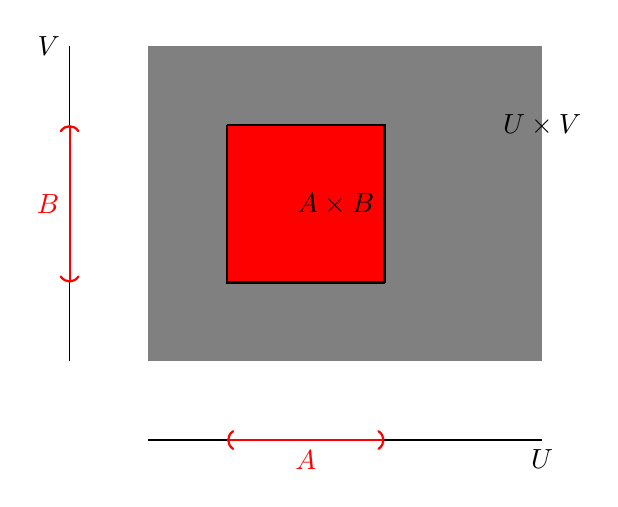
\begin{tikzpicture}[
    vec/.style={thick,[-)},
]
 
    \coordinate (A) at (2,0);
    \coordinate (B) at (0,2);
    \coordinate (cross prod) at (2,2);
    \def\tick{0.2}

    \draw [-] (1,0) -- (6,0) node [below] {$U$};
    \draw [-] (0,1) -- (0,5) node [left]  {$V$};

    \draw [(-),red, thick ] (2,0) -- ++(A) node [midway,below] {$A$};
    \draw [(-), red, thick ] (0,2) -- ++(B) node [midway,left]  {$B$};

    \fill [gray] (1,1) rectangle ++($(5,4)$) ;
    \draw (6,4) node  {$U \times V$};
    
   \fill [red] (cross prod) rectangle ++($(A)+(B)$);
    \draw [thick] ($(cross prod)+(A)$) -| ($(cross prod)+(B)$);
    \draw [thick] ($(cross prod)+(A)$) |- ($(cross prod)+(B)$)
        node [pos=0.25,left] {$A \times B$};
\end{tikzpicture} 
 
 
 For example if $A =\{1,2,3\}$ and $B = \{a\}$ then  $A\times B =\{(1,a), (2,a), (3,a)\}$.
 Note that from the point of view described in sections \ref{sec:sets} and \ref{sec:setsincoq},  if $A$ is of type Ensemble $U$ and $B$ is of type Ensemble $V$ then  $A\times B: Ensemble (U*V)$. Note also that $A*B$ is endowed with two projections fst:$A*B\rightarrow A$ and snd :$A*B\rightarrow B$. We use these to define:
 
 \inp{Definition prod ( U V:Type) (A :Ensemble U)(B:Ensemble V): Ensemble (U*V):=fun x=> ((fst x) $\in$ A $\land$ (snd x) $\in$ B) .}
 
 and
 \inp{Notation "A 'X' B":=(prod \_ \_ A B)( at level 40).}
 
 
 
 
 We also define a (binary relation) $A$ with domain $A$ and range $B$ as subset of $A\times B$. One can think of a relations as a way of associating elements form $A$ and  $B$. For example, assume that $A=\{a,b,c,d\}$ and $B=\{1,2,3,4\}$ and $R=\{(a,2), (a,3), (b,2), (c,3)\}$. We can represent this as:
 
 \begin{figure}
 \centering
 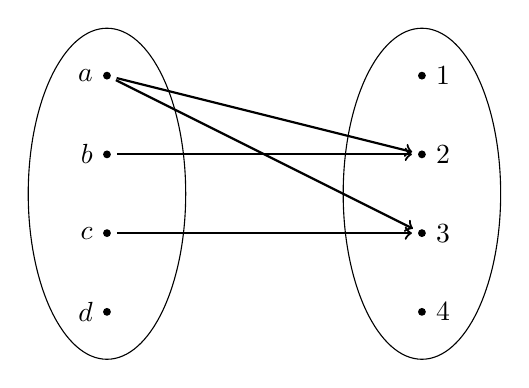
\begin{tikzpicture}[ele/.style={fill=black,circle,minimum width=.8pt,inner sep=1pt},every fit/.style={ellipse,draw,inner sep=-2pt}]
  \node[ele,label=left:$a$] (a1) at (0,4) {};    
  \node[ele,label=left:$b$] (a2) at (0,3) {};    
  \node[ele,label=left:$c$] (a3) at (0,2) {};
  \node[ele,label=left:$d$] (a4) at (0,1) {};

  \node[ele,,label=right:$1$] (b1) at (4,4) {};
  \node[ele,,label=right:$2$] (b2) at (4,3) {};
  \node[ele,,label=right:$3$] (b3) at (4,2) {};
  \node[ele,,label=right:$4$] (b4) at (4,1) {};

  \node[draw,fit= (a1) (a2) (a3) (a4),minimum width=2cm] {} ;
  \node[draw,fit= (b1) (b2) (b3) (b4),minimum width=2cm] {} ;  
  \draw[->,thick,shorten <=2pt,shorten >=2pt] (a1) -- (b2);
  \draw[->,thick,shorten <=2pt,shorten >=2] (a1) -- (b3);
  \draw[->,thick,shorten <=2pt,shorten >=2] (a2) -- (b2);
  \draw[->,thick,shorten <=2pt,shorten >=2] (a3) -- (b3);
 \end{tikzpicture}
\end{figure}

Relations can represent various real life connections. For example one can think of a relation with domain the set of all people and range the set of all cars where a pair $(a, b)\in R$ if the person $a$ has ever been in car $b$. We can also think of more mathematical relations, for example the relation $R$ with domain $\mathbb{R}$ and range $\mathbb{R}$ given by $(x,y)\in R$ and only if $y=x^2$. We sometimes call this relation the graph of the function $f:\mathbb{R}\rightarrow \mathbb{R}, f(x)=x^2$.
 
 \inp{Definition isrel ( U V:Type) (A :Ensemble U)(B:Ensemble V) (R:Ensemble (U* V)) $ :R\subseteq (A X B).$}
 
 Here is an example, let us define the relation less than with domain natural numbers and range all numbers larger than 1 and prove it is a relation. Note that we will not go into details about natural numbers here as we will do so in Chapter~\ref{ch:numbers}.
 
 \inp{
 Definition allnat:Ensemble nat: fun x=> True.\\
 Definition strictlypos:Ensemble nat := fun x=> x>0.\\
 Definition mylt:Ensemble nat*nat:= fun a => fst a < snd a.}
 
 Let us prove that melt is a relation with domain allnat and range strictlypos.
 \inp{Lemma a: isrel nat nat allnat strictlypos mylt.
 }
 
 The first few steps are just unfolding of definitions:
 \inp{
Rewrite goal using the definition of isrel.\\
Rewrite goal using the definition of Included.\\
Fix an arbitrary element a.\\
Assume (a $\in$ melt) then prove (a $\in$ (allnat X strictlypos)).\\
Rewrite hypothesis Hyp  using the definition of (In, mylt).\\
Rewrite goal using the definition of (In, prod).\\
Rewrite goal using the definition of (In, allnat).\\
Prove the conjunction in the goal by first proving True then (strictlypos (snd a)).
This is trivial.\\
Rewrite goal using the definition of strictlypos.}

We are now left with the goal
\coq{a:nat * nat\\
Hyp: fst\ a < snd\ a
}{0 < snd \  a}


We now try to search for some useful theorem, one that implies that 0 is smaller than something:
\inp{SearchPattern (( \_ -> 0 <  \_ )).}

The result includes

\mess{Nat.lt\_lt\_0: $\forall n m : nat, n < m \rightarrow 0 < m$}

And so if we do

\inp{Apply result (Nat.lt\_lt\_0  (fst a) (snd a)).}

We only need to use the assumptions.

On the other hand 

On the other hand,  mylt is not a relation with domain strictlypositive.

\inp{Lemma a: not ( isrel nat nat  strictlypos  allnat mylt).}

We can prove this by first unfolding some definitions:

\inp{Rewrite goal using the definition of not.\\
Assume (isrel nat nat strictlypos allnat mylt) then prove False.\\
Rewrite hypothesis Hyp  using the definition of isrel.\\
Rewrite hypothesis Hyp  using the definition of Included.
}

To get

\coq{Hyp: \forall  x : nat * nat, (x \in mylt) \rightarrow (x \in (strictlypos \times allnat)))}{False}



Now we choose the element $(0,1)$ and we show that $(0,1) \in mylt$ and $(0,1)\not\in  (strictlypos \times allnat))$ obtaining a contradiction.

The proof of 
 $(0,1) \in mylt$ is very easy:
 \inp{Claim ((0,1) $\in$ mylt).
Rewrite goal using the definition of (In, mylt).
This is trivial.}

The proof of $(0,1)\not\in $ (strictlypos $\times$ allnat))  is a bit harder:

\inp{Claim (not ((0,1) $\in$ (strictlypos $\times$ allnat))).\\
Rewrite goal using the definition of (In, prod).\\
Rewrite goal using the definition of (In, strictlypos).\\
Rewrite goal using the definition of allnat.\\
Rewrite goal using the definition of not.\\
Assume (0  <  fst  (0,  1)  $\land$  True  ) then prove False.\\
Eliminate the conjuction in hypothesis Hyp0.\\
Claim (0<0) by rewriting H0 using (fst (0,1)).}
At this point we have:

\coq{Hyp: (\forall x : nat * nat, (x \in mylt) \rightarrow (x \in (strictlypos \times allnat)))\\
H:(0,1) \in mylt \\
H0: 0 <fst (0,1)\\
H1:True\\
H2:0 < 0}{False}

And we look for a theorem about not (\_<\_)

\inp{SearchPattern (not (\_< \_))}.

To get \mess{Nat.nlt\_0\_r: $\forall$ n : nat, $\neg n < 0$}

We then apply this theorem and the rest is straightforward.
\inp{Apply result  (Nat.nlt\_0\_r  0 H2).\\
Apply result H0 .\\
Apply result Hyp .\\
This follows from assumptions.}

\section{Binary relations on a set}\label{sec:binaryrelations}

There is an especially important subclass of general relations. If A is a type, a binary relation on $A$ is a subset of $A\times A$. This concept includes many examples you already know. Here are some natural examples:
\begin{enumerate}
\item  if $A$ is any set the relation of equality can be viewed as the set $$\{ (a,a) | a \in A\}$$.  
\item If the set $A$ is some subset of real numbers you can define the relation of order $$\{ (a, b) \mid a , b \in A \land a<b\}$$. 
\item If $A= \mathbb{Z}$ you can define divisibility  relation $$\{ (a, b) \mid a, b \in \mathbb{Z} \land  a | b \}$$
\item if $A= \mathbb{Z}$  you can define the ``= mod 3'' relation as the set:
$$\{(a, b) \mid alb \in \mathbb{Z} \land 3 | a-b \}$$
\item if $A$ is the set of all people you define two people to be related if they are from the same family.
\end{enumerate}
We now describe things in Spatchcoq. For simplicity, in this section the set $A$ will be fixed and we will see relations not as in \ref{subsec:defin of cartesian}  but as predicates of two variables, that is as elements of type $A \rightarrow A \rightarrow Prop$. For that end we will use directly the package Relations in Coq.

\inp{Require Import Relation}

For example, we can define the equality relation on a  type $A$ as
\inp{Definition eq (A:Type): relation A: fun a b => a=b.}

You can (re)define  the order on natural numbers as :
\inp{Definition mylt:relation nat: fun a b => a<b.}

Divisibility can be defined as:
\inp{Local Open Scope Z\_scope.\\
Definition div:relation Z: fun a b => exists c:nat,  b= a*c.}

And we can define the mod 3 on $\mathbb Z$ as

\inp{Definition mod3:relation Z: fun a b => div 3 (a-b).}

\warn{Note that for the definitions above I needed the integers and not the natural numbers, if we defined this in the natural numbers you will run into troubles regarding  minus as in in \ref{subsec:warnings} }

For simplicity very often we will also use the following common notation: if $R$ is a relation on the set $A$ and $(a,b)\in R$ we will write $a R b$.

Some relations have certain properties that are useful. We list them in the definition bellow. 
\begin{definition}[reflexive]
A relation $R \subseteq A\times A$ is {\it reflexive} if $\forall a \in A, a Ra$, that is any element is related to itself.
\end{definition}

Note that this definition is already there
\inp{Print reflexive.} 
gives

\mess{reflexive = 
$\lambda$ (A : Type) (R : relation A), $\forall$  x : A, R x x
}

For example equality and =mod3  are reflexive relation but `` < '' is not. Here is a proof for mod3

\inp{Lemma a:reflexive Z mod3.}
\begin{proof}[informal]
We need to show that $forall x \in \mathbb{Z}, mod3 x x$. We fix a $x$ and rewrite the definition of mod3. We therefore need show that $div 3 (x-x)$. If we rewrite  the definition of divide we need to show that $\exists c \in \mathbb{Z}, (x-x) = 3c$. It remains to pick $c=0$.
\end{proof}
\begin{proof}[formal]
\inp{
Rewrite goal using the definition of reflexive.\\
Fix an arbitrary element x.\\
Rewrite goal using the definition of mod3.\\
Rewrite goal using the definition of div.\\
Prove the existential claim is true for 0.\\
True by arithmetic properties.\\
}\end{proof}

 \begin{definition}[symmetric]
A relation $R\subseteq A\times A$ is {\it symmetric} if $\forall a b\in A, a R b \rightarrow b R a$.
\end{definition}

As before:
\inp{Print symmetric.}

Gives
\mess{symmetric = $\lambda$ (A : Type) (R : relation A), $\forall$ x y : A, R x y $\rightarrow$ R y x}


We will now prove that mod3 is also symmetric:
\inp{
Lemma a:symmetric Z mod3.}
\begin{proof}[informal]
We need to show that $forall x y \in \mathbb{Z}, mod3 x y \rightarrow mod3 y x$. To do so we fix $x$ and $y$ and use the definitions of mod3 respectively div. We are left to prove that $\exists c : Z, x - y = 3 * c\rightarrow \exists c : Z, y - x = 3 * c$ and so we assume that $\exists c : Z, x - y = 3 * c$ and prove that $\exists c : Z, y- x = 3 * c$ if we pick the c so that $x-y =3c$ then it is not too hard to see that $y-x = 3(-c)$.
\end{proof}
The formal proof is slightly harder.

\begin{proof}[formal]


\inp{
Rewrite goal using the definition of symmetric.\\
Fix an arbitrary element x.\\
Fix an arbitrary element y.\\
Rewrite goal using the definition of mod3.\\
Rewrite goal using the definition of div.\\
Assume ($\exists$ c : Z, x - y = 3 * c) then prove ($\exists$ c : Z, y - x = 3 * c).\\
Fix c the existentially quantified variable in Hyp .\\
Prove the existential claim is true for (-c).\\
Replace (3 * c) by (x - y) in the goal.\\
Claim (3*(-c)= -(3*c)).\\
True by arithmetic properties.\\
Rewrite the goal using H .\\
Replace (3 * c) by (x - y) in the goal.\\
True by arithmetic properties.}
 \end{proof}
 
 Note that the ``Claim (3*(-c)= -(3*c)).'' is needed here while it was implicitely used in our informal proofs.
 
 
 
  \begin{definition}[transitive]
A relation $ R \subseteq A\times A$is {\it transitive} if $\forall a b c\in A, a R b \land b R c \rightarrow a R c$.
\end{definition}

However 
\inp{Print transitive.}

Gives
\mess{transitive= $\lambda$ (A : Type) (R : relation A), $\forall $ x y z : A, R x y $\rightarrow$ R y z $\rightarrow$ R x z}

This looks a bit different but the two are equivalent. See for example exercise andimp ar page \pageref{prop:exercises}.


Let us prove that mod3 is transitive
\inp{Lemma trans: transitive Z mod3.}
\inp{
Rewrite goal using the definition of transitive.\\
Fix an arbitrary element x.\\
Fix an arbitrary element y.\\
Fix an arbitrary element z.\\
Rewrite goal using the definition of mod3.\\
Rewrite goal using the definition of div.\\
Assume ($\exists$ c : Z, x - y = 3 * c) then prove \\ (($\exists c : Z, y - z = 3 * c) \rightarrow (\exists c : Z, x - z = 3 * c)).$\\
Assume ($\exists$ c : Z, y - z = 3 * c) then prove ($\exists$ c : Z, x - z = 3 * c).\\
Fix c the existentially quantified variable in Hyp .\\
Fix d the existentially quantified variable in Hyp0 .\\
Prove the existential claim is true for (c+d).\\
Claim (3*(c+d)= 3*c+3*d).\\
True by arithmetic properties.\\
Replace (3 * (c + d)) by ((3 * c) + (3 * d)) in the goal.\\
Replace (3 * c) by (x - y) in the goal.\\
Replace (3 * d) by (y - z) in the goal.\\
True by arithmetic properties.}
 
 \section{Functions}\label{sec:functions}
 
\include{SetTheory/finsets}

\chapter{Algebraic Structures}\label{ch:algstr}

This Chapter proposes to raise the level of abstraction that you encounter. I hope that  the abstract concepts you already encountered via SpatcCoq will help the transition. We will describe general abstract concepts and note  many of the notions encountered in the previous sections appear as special cases. This way of doing mathematics is almost as old as civilisation itself. Throughout the ancient world scholars made various attempts at abstraction in order to formulate general solutions to practical or theoretical problems. We can see that in Babilonian solutions to quadratic equations\cite{Robson:2002aa}, the geometric algebra of Eyipt   \cite{robins1987rhind}, Greece \cite{Euclid:2002aa} and China \cite{abbott_2001}. It was not until Diophantus and Muhammad ibn Musa al-Khwaarizm\`i that the fundamentals of formal algebra started to emerge. They will be completely formalised by Viete and Descartes in the 16th and 17th century. See \cite{Shell-Gellasch:2015aa} and \cite{Waerden:1983aa} for excellent historical records of the development of algebra.

In the 19th and 20th century Algebra saw a complete rejuvenation. A general idea started to crystallise, general abstract structures can be defined and described and results about those structures  will then specialised to many areas of Mathematics. Abstract or Modern Algebra was born. A plethora of such structures appeared, groups, rings, fields, algebras and, more recently categories. This book will not even scratch  the surface of the rich and beautiful field. The interested reader should run to the nearest library and borrow a copy of Shafarevich's gem \cite{Shafarevich:2006aa} and read it before the week is over.

Some of the most resounding successes of Proof assistants were in the realm of Abstract Algebra. Indeed the large effort of Gonthier  and his team lead to the formalisation of the Odd Order Theorem, one of the most difficult theorems in the Classification of Finite Simple Groups. I am a huge admirer of Mathematical Components and ssreflect. Unfortunately, I think that while they are  beautiful and effective theier austerity makes them a bit unsuitable for teaching at this level. The more advanced reader should definitely check the gorgeous book by Assia Mahboubi and Enrico Tassi( with contributions by Yves Bertot and Georges Gonthier) \cite{MathComp}. I will restrict to the vanilla version of Coq and will sacrifice elegance and briefness for the sake of clarity. Moreover, as these are not standard subjects in a discrete Mathematics course, each section will be separated in two almost mirroring subsections. The first will be entirely informal and the second entirely formal.
\section{Groups}

Group theory is one of the oldest subjects in what we now call Abstract Algebra. We now like to describe groups as arbiters of symmetry in any of guises from geometric tiling patterns to chemical molecules. However it was not always so. Groups were invented by Evariste Galois in the 19th century as a bookkeeping system  for the express purpose of solving polynomial equations. In a series of mind-shaterring papers, the 19 year old developed a correspondence between  polynomial equations and a completely new set of beasts: Permutation Groups. He then started to study this new bestiary, identified  those that will help solve equations and showed that some equations are just not solvable. Then he spent 6 months in prison for being a republican and promptly died in a mysterious duel. The absolute romantic figure if there ever was one. Recently Peter Neumann has collected all his works in a very interesting book\cite{Galois:2011aa}.

 A mere 40 years afterwards, Felix Klein presented the world with the Ernlangen Program \cite{klein1893} in which he  proposed to classify geometric objects via their symmetries. In the intervening 150 years, Groups have found applications in many areas of Mathematics, Physics, Chemistry and Computer Science  and even in Childhood Psychology \cite{piaget1960logic}.  Moreover, in the 1970's ``the building blocks '' of finite groups have been classified. This is one of the most spectacular endeavours of human culture. An concerted effort by quite a few dozens of mathematicians produced a 10000 page proof of the statement: ``We now the stuff that groups are made of! ''. There are some (infinitely many) families of related and nicely behaved groups and 26 ``sporadic`` ones.'''' 
 
 Our treatment will be brief and somewhat formal. The reader should not expect to really learn moderne Group Theory from the short section.  For a more in depth analysis the reader is directed to a more standard Group theory book such as \cite{scott2012group} or a more exciting popularisation book such as \cite{Sautoy:2009aa,Sautoy:2012aa, Ronan:2007aa}

\subsection{Definitions and first theorems(informally).}
A group is a set together with a binary operations that satisfies some natural properties. The reader should take as the standard first example the set of integers together with the operation $+$ and as the standard ``non-examples'' the same set with operations $-$ or $*$. 

We will now define abstract groups. Our choice  definition might sound strange to the expert. We start with a mysterious larger set $U$, define the multiplication a bit more generally and do not ask for left identity or left inverses. We make this choice in order to optimise the formalisation and the effort of verifying that an object is a group. We will the proceed to show the equivalence with the standard definitions and prove some standard properties of a group. 
\begin{definition}\label{def:group}
A group is a triple $(G, mult, e_G, inv)$ where $G\subset U$ is a set, $mult: U\times U \rightarrow U$ is a binary operation that associates to every pair of elements $ a,  b $ an element $mult\ a\ b$,  $e$ is an element of  $U$ and $inv:U\rightarrow  U$ is a function. In order to simplify notations we will denote $mult( a,  \ b)$ by $ a* b$ and $inv(x)$ by $x^{-1}$. The triplet has to satisfy the following:
\begin{itemize}
\item {\bf mult\_closure}
G is closed under multiplication, that is $\forall a\  b \in G,  a * b \in G$.
\item {\bf assoc} $\forall x\  y\ z\in G, (mult\ x\ y) z = mult \  x (mult\  y\ z)$, that is $(x * y) * z = x* (y*z)$.
 \item {\bf right\_id} $ \forall x\in G ,  mult\  x\  e_{G} = x* e_{G}= x$
 \item {\bf inv\_closure} $\forall x\in G,  x^{-1} \in G$
   \item {\bf right\_inverse} $\forall x \in G,  mult\ x (inv\ x) = x* x^{-1} =  e_{G}$
\end{itemize}
\paragraph[\bf First examples and counterexamples]{
Consider $U=G =\mathbb{Z}$.
\begin{itemize}
\item Show that if $mult: \mathbb{Z} \times \mathbb{Z} \rightarrow \mathbb{Z}$ is defined as $mult( x, y) = x+y$ then you can find $e_\mathbb{Z}$ and $inv: \mathbb{Z} \rightarrow \mathbb{Z}$ so that $(\mathbb{Z}, mult, e_{\mathbb{Z}}, inv)$ is a group.
\item Show that if $mult: \mathbb{Z} \times \mathbb{Z} \rightarrow \mathbb{Z}$ is defined as $mult (x, y) = x*y$ then you {\bf cannot} find $e_\mathbb{Z}$ and $inv: \mathbb{Z} \rightarrow \mathbb{Z}$ so that $(\mathbb{Z}, mult, e_{\mathbb{Z}}, inv)$ is a group.
\item Show that if $mult: \mathbb{Z} \times \mathbb{Z} \rightarrow \mathbb{Z}$ is defined as $mult (x, y) = x-y$ then you  {\bf cannot}  find $e_\mathbb{Z}$ and $inv: \mathbb{Z} \rightarrow \mathbb{Z}$ so that $(\mathbb{Z}, mult, e_{\mathbb{Z}}, inv)$ is a group.
\end{itemize}}
\end{definition}

Note a more standard definition of a group:
\begin{definition}\label{def:gpshorted}
A group is a pair $(G, *)$ where $G$ is a set and $*:G\times G \rightarrow G$ is a function such that:\
\begin{itemize}
\item {\bf associativity} $\forall x, y,z \in G, (x * y) * z = x* (y*z)$.
\item {\bf identity} There exists $e_{G}\in G$ so that $\forall x \in G, x* e_{G}= e_{G}*x = x$.
\item {\bf inverse} Every element has an inverse, that is $\forall x \in G, \exists y \in G, x*y = y*x =e_{G}$.
\end{itemize}

\end{definition}

The two definitions seem slightly different but we will soon show that they are in fact equivalent. Note first that a pair $(G,*)$ that satisfies the condition of Definition \ref{def:gpshorted} can be easily seen to be extended to a triplet that satisfy Definition \ref{def:group}. Indeed take $U=G$, $mult = *$, $e_{G}$ the element defined by identity condition and $inv(x)$ to be an element $y$ that satisfies the condition inverse. It is left as an exercise that this choice satisfy Definition \ref{def:group}. From now  a group will be a triplet $(G, mult, e_{G}, inv)$ as defined in Definition \ref{def:group}.

We first show that the element $e_{G}$ is unique with that property. In fact we shall prove something stronger: the only  element with  the property that its square is identical to itself ( this is called an idempotent in algebra) is the identity.

\begin{lemma}[unit\_uniq]\label{leminf:unituniq}
If $(G, mult, e, inv)$ is a group then $\forall x \in G, x* x = x \rightarrow x=e$.
 \end{lemma}
\begin{proof}[informal]
We need to show that $x*x = x \rightarrow x =e$. To do so assume $x*x=x$ and  try to prove that $x=e$. Note that, by the definition of the identity we have $x= x*e$ and so the goal is equivalent to proving that $x * e = e$. We now also note that $x*x^{-1}= e$ and so the goal is equivalent to $x* (x* x^{-1}) = e$. You can use associativity to see that it is enough to prove that $(x*x)* x^{-1} =e$. Nor by assumption we know that $x*x =x$ and , replacing $x*x$ by $x$  in the goal we only need to show $x*x^{-1}= e$ which is exactly the property of the right inverse.
\end{proof}

Next we are able to prove that right inverses are also left inverses :
\begin{lemma}[ left\_inverse] ~$\forall x, x^{-1} * x =e_{G}.$
\end{lemma}
\begin{proof}
To see that let us fix an $x$. We will use Lemma\ref{leminf:unituniq} for $y=x^{-1}* x$. This means that, in order to show that $y=e_{G}$,  it is enough to show that $y.* y= y$. Now  we repeatedly use associativity as well as right\_inverse and right\_id:
\begin{align*}
y* y & =  (x^{-1}* x)*(x^{-1}*x )= x^{-1}* (x* (x^{-1}*x )) =x^{-1}*(( x* x^{-1})* x ) \\ & = x^{-1}* (e_{G}* x)=(x^{-1}* e_{G})* x= x^{-1}*x \\ & =  y
\end{align*}
\end{proof}

We can now prove that the right identity is also a right identity, that is:

\begin{lemma}[left\_id]$\forall x, e_{G}*x =x.$
\end{lemma}
\begin{proof}
Let us fix an element $x$. Using the right\_inv and assoc  properties we get that $$e_{G}* x= (x* x^{-1})*x= x* (x^{-1}*x)$$
Next we can use left\_inverse lemma and the right\_id we get  get  $x*(x^{-1}*x)= x* e_{G}=x$. Combining the two equalities we get
$e_{G}* x= x$.
\end{proof}

And the fact that the inverse of an element is unique:
\begin{lemma}[inverse\_uniq] $\forall x y, x*y = e-> y = x^{-1}.$
\end{lemma}
\begin{proof}
Fix $x $ and $y$ and assume $x*y = e$. We need to show that $y=x^{-1}$.
Note that
$$ y =e_{G} * y = (x^{-1}* x)* e_{G}= x^{-1}*(x*y) = x^{-1}* e_{G}= x^{-1} $$

\end{proof}


We can also show that, in a group, you have right cancelation:

\begin{lemma}[right\_cancel] $\forall x\  y\  z, x*y= z*y-> x=z.$\
\end{lemma}
\begin{proof}
We fix $x, y$ and $z$,  assume $x*y= z*y$ and prove $x=z$.

Now we have that
$$ x = x*e_{G}= x* (y * y^{-1})=(x*y)* y^{-1}= (z*y)*y^{-1}= z*( y* y^{-1}) = z*e_{G}= z $$
\end{proof}

\subsection{Definitions and first theorems(formal with Typeclasses)}

In this section we formalise groups and reprove the lemmas above, this time in spatchcoq. You should see the similarities.
To introduce  a group we will use some new Coq notions, Casses and  Instants .  
We start by importing Ensembles and  recalling the set notations:
\inp{
Require Import Ensembles.\\
Notation "x $ \in $ A":= (In \_ A x) (at level 10).\\
Notation "A $ \subseteq $ B":= (Included \_  A B)(at level 10).\\
Notation "A $\cup$ B":= (Union \_  A B)(at level 8).\\
Notation "A $ \cap $ B" := (Intersection \_  A B) (at level 10).}
We now start a module. This is convenient for polymorphisms. 
\inp{
Module gps.}

The definition of a groups will resemble Definition~\ref{def:group} closely. However we are not using a definition but a class notation. 
\inp{ 
Class Group (U:Type) (set : Ensemble U) := \\
  \{op:  U->U->U;\\
   inv :  U->U;\\
    e:U;\\
 mult\_closure : forall x y:U, In U set x -> In U set y -> In U set  (op x y);\\
   assoc : forall x y z:U,  op (op x y) z = op  x (op y z);\\
   id\_closure : In U set e;\\
   right\_id : forall x:U, op x  e = x;\\
   inv\_closure : forall x:U,  In U set (inv x);\\
   right\_inverse: forall x:U, op x (inv x) =  e;\\
  \}.}
In CS this  is called  a ``Type class''. It is a concept first introduced in Haskell in order to enable overloading of arithmetics  operations. A group will be a type class that depends of two parameters, a type (U:Type) (the overset of the group) and a set:Ensemble U that is the actual underlying set of G. We could have exaggerated a bit and defined U and set inside the Class but we wanted some parameters.A group will also have an operation  which is a function of two variables $op: U\rightarrow U \rightarrow U$, an inverse $inv:U \rightarrow U$ and an identity $e:U$. It has to satisfy the properties in Definition~\ref{def:group}. In fact the definition is in some sense an inductive constructor, not unlike $nat$. Note that the Class introduction creates some ``projection functions'' as well. For example try
\inp{Check op.}
 And note that you get:
 \mess{op\\
     : ?U $\rightarrow$
 ?U $\rightarrow$
 ?U\\
where\\
?U : [ $\vdash$ Type] \\
?set : [ $\vdash$ Ensemble ?U] \\
?Group : [ $\vdash$ Group ?U ?set] }

This is a strange looking message isn't it? It means that op is now a dependent function. It depends of what the ``flavour of the month'' is in groups. As we will see soon, once we have an instance of a group then the same Check will give a completely different answer.

Since we know op and inv we  also introduce some convenient notations:
\inp{Notation "x '.*' y" := (op x y) (at level 40, no associativity).\\
Notation "x\inv'" := (inv x ) (at level 20).}

Note that we could have overloaded the $*$ notation. This might run into some difficulties and so we use the notation ``.*''. We also require no associativity so that Coq does not save on brackets.

Once we defined a group, we can immediately start proving theorems about it.

A general theorem about groups will look as follows:
\inp{
Lemma name \`{}\{G:Group\}: P}

Where P is a proposition involving $e, .*, x\inv $. Note the format \`{}\{G:Group\}, this is a shortcut called implicit generalisation. It generalises everything it can. For example let us prove the uniqueness of identity (we shall prove the theorem inside the module gps so we can use it with any group.


\inp{
Lemma unit\_uniq  \`{}\{G:Group\}: forall x ,  x .* x = x $\rightarrow$ x = e.}

The resulting goal is 
\coq{U:Type\\ set: Ensemble\ U\\
G: Group\ U\ set}{\forall   x  :  U,  x  .*  x  =  x  \rightarrow  x  =  e }
Note that even if we never spoke of U or set, they have been chosen for us (generalised) by the notation. 

\rmk{
We could have employed this earlier, for example
\inp{Generalizable All Variables.\\
Lemma a:\`{}(m+n = n+m).}

Will generalise m and n in the context, 

\coq{ }{\forall m\  n:nat, m+n=n+m.}


We chose not to do so earlier to keep notations light. Nevertheless here the notations are already heavy and this will be slightly easier.}

The first two moves are standard.
\inp{
Fix an arbitrary element x.\\
Assume (x  .*  x  =  x) then prove (x=e).}

And we arrive at 
\coq{U:Type\\ set: Ensemble\ U\\
G: Group\ U\ set\\  x  : U \\  Hyp: x  .*  x  =  x}{   x  =  e }
We will now use the fact that $x = x*e$ and we replace it in the goal (and prove it later)

\inp{
Replace x by (x {*} e)  in the goal.}
\coq{U:Type\\ set: Ensemble\ U\\
G: Group\ U\ set\\  x  : U \\  Hyp: x  .*  x  =  x}{   x .* e =  e }
Respectively
\coq{U:Type\\ set: Ensemble\ U\\
G: Group\ U\ set\\  x  : U \\  Hyp: x  .*  x  =  x}{   x .* e =  x }
  We now know that  x.* x \inv = e and so 
  \inp{Replace e by (x*x\inv) in the goal.} gives 
\coq{U:Type\\ set: Ensemble\ U\\
G: Group\ U\ set\\  x  : U \\  Hyp: x  *  x  =  x}{x  {*}  (x  {*}  x\inv)  =  x  {*}  x\inv }
 
 Respectively 
 \coq{U:Type\\ set: Ensemble\ U\\
G: Group\ U\ set\\  x  : U \\  Hyp: x  *  x  =  x}{x  {*}  x\inv  =  e }

We now apply associativity and Hyp. 
\inp{
Rewrite the goal using assoc.\\
Rewrite the goal using Hyp .\\
This follows from reflexivity.}

And we now only need to show the two goals that we introduced.
\inp{
Apply result right\_inverse.\\
Apply result right\_id.\\
Qed.}
Let us now reprove the left\_inv lemma:
\inp{
Lemma left\_inverse \`{}\{G:Group\}: forall x, x\inv
 .* x =e.}
 We prove it almost the same way as the informal version. We first fix an element $x$ and use unit\_uniq.
\inp{Fix an arbitrary element x.\\
Apply result unit\_uniq.}

The result is:
 \coq{U:Type\\ set: Ensemble\ U\\
G: Group\ U\ set\\  x  : U \\  Hyp: x  *  x  =  x}{(x\inv  .*  x)  .*  (x \inv  .*  x)  =  x\inv  .*  x ) }
We now use assoc
\inp{Rewrite the goal using assoc.}
to get

 \coq{U:Type\\ set: Ensemble\ U\\
G: Group\ U\ set\\  x  : U \\  Hyp: x  *  x  =  x}{(x\inv  .*  (x  .*  (x \inv  .*  x) ) =  x\inv  .*  x ) }

Now it would be very tempting to apply associativity again. Nevertheless, due to the way we defined the apply tactic if we do so we will be back where we started and so we need to be precise on how we want to use it:
\inp{
Replace (x  .*  (x  \inv
  .*  x) ) by ((x .*  x  \inv
)  .*  x) in the goal.}

And we get 
\coq{U:Type\\ set: Ensemble\ U\\
G: Group\ U\ set\\  x  : U \\  Hyp: x  *  x  =  x}{x\inv  .*  (x  .*  x \inv)  .*  x ) =  x\inv  .*  x ) }

And another (easy) goal to be proved later

\coq{U:Type\\ set: Ensemble\ U\\
G: Group\ U\ set\\  x  : U \\  Hyp: x  *  x  =  x}{x  .*  (x  \inv
  .*  x) =(x .*  x  \inv
)  .*  x  }

\inp{Rewrite the goal using right\_inverse.\\
Rewrite the goal using assoc .}

And we have
\coq{U:Type\\ set: Ensemble\ U\\
G: Group\ U\ set\\  x  : U \\  Hyp: x  *  x  =  x}{ (x  \inv
  .*  e).* x =x \inv .*  x  }
  
  This can easily be proved by:
  \inp{
Rewrite the goal using right\_id.\\
This follows from reflexivity.}


Leaving just the new goal to prove:
\inp{
Rewrite the goal using assoc.\\
This follows from reflexivity.\\
Qed.}

We will not go through the rest of the proofs step by step, try them for yourself.



\inp{
Lemma left\_id \`{}\{G:Group\}: forall x, e.*x =x.\\
Fix an arbitrary element x.\\
Rewrite the goal using (right\_inverse x).\\
Rewrite the goal using assoc.\\
Rewrite the goal using left\_inverse.\\
Rewrite the goal using right\_id.\\
This follows from reflexivity.\\
Qed.}



\inp{
Lemma inverse\_uniq \`{}\{G:Group\}: forall x y, x.*y = e-> y = x\inv
.\\
Fix an arbitrary element x.\\
Fix an arbitrary element y.\\
Assume (x  .*  y  =  e ) then prove ( y  =  x  \inv
 ).\\
Rewrite the goal using right\_id.\\
Rewrite the goal using Hyp.\\
Rewrite the goal using assoc.\\
Rewrite the goal using left\_inverse.\\
Rewrite the goal using left\_id.\\
This follows from reflexivity.\\
Qed.}\inp{
Lemma right\_cancel  \`{}\{G:Group\}: forall x y z, x.*y= z.*y-> x=z.\\
Fix an arbitrary element x.\\
Fix an arbitrary element y.\\
Fix an arbitrary element z.\\
Assume (x .* y = z .* y) then prove (x = z).\\
Replace x by (x.*e) in the goal.\\
Rewrite the goal using (right\_inverse y).\\
Rewrite the goal using assoc.\\
Replace (x .* y) by (z .* y) in the goal.\\
Rewrite the goal using assoc.\\
Rewrite the goal using right\_inverse.\\
Rewrite the goal using right\_id.\\
This follows from reflexivity.\\
Rewrite the goal using right\_id.\\
This follows from reflexivity.\\
Qed.}
We now close the Module gps. 
\inp{
End gps.}


After proving some general results, we now show how to define a particular group. We shall see that $\mathbb{Z}$ is a group under addition. We first import the module we just closed.
\inp{
Import gps.}
Next we use the Instance command. This defines a group following the pattern in the Class. You need to give a type and a Ensemble set. IN this case we pick $\mathbb{Z}$ respectively the whole $\mathbb{Z}$ as set, more precisely set =$fun  x \Rightarrow True.$ We also give the variable op, inv and e.
\inp{
Instance  s:Group Z (fun  x=>True):=\{op:= Z.add; inv:= Z.opp; e:= 0\}.}

Note that the result is that we have to prove 6 different goals, the ones that were promised in the Class description: mult\_closure, assoc, id\_closure,  right\_id, inv\_closure, right\_inverse. The definition is interactive. We need to prove them one by one.


\inp{
Rewrite goal using the definition of In.}
The result is quite bizarre:
\coq{ }{(Z \rightarrow
 (Z \rightarrow
 (True \rightarrow
 (True \rightarrow
 True))))}
 This is an unfortunate shortcut in Coq. Whenever the variable is unimportant, the expression $x:Z$ is shortened to just $Z$. Nevertheless this is a trivial statement. The rest are either trivial or applications of standard lemmas:	
 
 \inp{
This is trivial.\\
Apply result Zplus\_assoc\_reverse.\\
Rewrite goal using the definition of In.\\
This is trivial.\\
Apply result Zplus\_0\_r.\\
Rewrite goal using the definition of In.\\
This is trivial.\\
Fix an arbitrary element x.\\
True by arithmetic properties.\\
Defined.}
Note that we end the proof with Defined rather than Qed. This allows the operations to be transparent. From now on, until we construct another instance, the only group in the world is $\mathbb{Z}$ under addition.

And we can see that one can apply unit\_uniq immediately.
\inp{
Lemma b: forall x:Z, x .* x = x -> x = e.\\
Apply result (unit\_uniq  Z s).\\
Qed.}

Note also that now .* means addition in $\mathbb Z$. Indeed:
\inp{Eval compute in 3\%Z .* 4\%Z.}
gives:

\mess{     = 7\%Z\\
     : Z}

While 
\inp{Eval compute in (3\%Z*4\%Z).}

Gives
\mess{   = 12\%Z\\
     : Z}

\begin{enumerate}
\item Show that any group admits left cancelation. That is
\inp{Lemma left\_cancel \`{}\{G:Group\}: $\forall x\ y\ z, y.*x= y.*z-> x=z.$
}
\item Show that in any group the socks and shoes property holds: \inp{Lemma socks\_shoes \`{}\{G:Group\}: $\forall x\  y , (x.*y)\inv= y\inv.*x\inv.$}
\item Prove the following Lemma:
\inp{Lemma inv \`{}\{G:Group\}: $\forall x \  y , (x.*x = e) \land  (y*y = e) \land ((x.* y).*(x.*y)=e)\rightarrow (x.*y = y.* x).$}

\end{enumerate}


%\subsection{with just records}
%Note that we gave been deliberately vague in assoc, right\_id and right\_inverse. This is because we will be somewhat light on this in our definition. We also did not require left inverses or left identity, we shall prove these later.
%
%To introduce the definition of a group we will use some new Coq notions, modules and  records.  
%We start by Importing sets and  recalling the set notations
%\inp{
%Require Import Ensembles.\\
%Notation "x $ \in $ A":= (In \_ A x) (at level 10).\\
%Notation "A $ \subseteq $ B":= (Included \_  A B)(at level 10).\\
%Notation "A $\cup$ B":= (Union \_  A B)(at level 8).\\
%Notation "A $ \cap $ B" := (Intersection \_  A B) (at level 10).}
%We now start a module. This is convenient for polymorphisms.
%\inp{
%Module gps.}
%
%The definition of a groups resembles Definition~\ref{def:group} closely. 
%\inp{ 
%Record Group : Type := group\\
%  \{U:Type;\\
%setG : Ensemble U;\\
%   mult : U -> U -> U;\\
%   inv : U -> U;\\
%   id : U;\\
%   mult\_closure : $\forall x y:U,  x \in setG \rightarrow y \in setG  \rightarrow  (mult x y) \in setG ;$\\
%   assoc : $\forall x y z:U,  mult\ (mult\ x\ y)\ z = mult\  x (mult\ y\ z);$\\
%   id\_closure : id $\in$ setG;\\
%   right\_id :$\forall x:U, mult\ x\  id = x;$\\
%   inv\_closure : $\forall x:U,  (inv\ x) \in setG;$\\
%   right\_inverse: $\forall x:U, mult\ x (inv\ x) =  id;$
%  \}.}
%  
%Note the format, this is in fact an inductive constructor, not unlike $nat$. 
%
%We introduce some convenient notations:
%\inp{
%Notation "x \{*\}  y":=(mult  \_ x y) (at level 50).\\
%Notation "'e'":=(id  \_ ) (at level 50).\\
%Notation "x \textasciicircum-1'":=(inv \_ x) (at level 30).}
%
%And we are now ready to prove the first group theory lemma, the uniqueness of identity (we shall prove the theorem inside the module gps so we can use it with any group.
%Note the lemma we need to prove is 
%\begin{lemma}
%In any group $G$, the identity is unique.
%\end{lemma}
%\begin{proof}[informal]
%To prove this we assume that another element $x$ is also an identity, that is $\forall y, x*y =y$. We do not need such generality, we shall show that $x*x = x \rightarrow x =e$. To do so assume $x*x=x$ and  try to prove that $x=e$. Note that, by the definition of the identity we have $x= x*e$ and so the goal is equivalent to proving that $x * e = e$. We now also note that $x*x^{-1}= e$ and so the goal is equivalent to $x* (x* x^{-1}) = e$. Youcan use associativity to see that it is enough to prove that $(x*x)* x^{-1} =e$. Nor by assumption we know that $x*x =x$ and , replacing $x*x$ by $x$  in the goal we only need to show $x*x^{-1}= e$ which is exactly the property of the right inverse.
%\end{proof}
%We shall prove this using SpatchCoq:
%
%\inp{
%Lemma unit\_uniq (U:Type)(G:Group): forall x:gps.U G, x \{*\} x = x -> x = e.}
%The ``gps:U G'' notation looks a bit strange but this automatically generated.
%
%The resulting goal is 
%\coq{U:Type\\ G:Group}{\forall   x  :  gps.U \ G,  x  \{*\}  x  =  x  \rightarrow  x  =  e }
%The first two moves are standard.
%\inp{
%Fix an arbitrary element x.\\
%Assume (x  \{*\}  x  =  x ) then prove (x=e).}
%
%And we arrive at 
%\coq{U:Type\\ G:Group \\  x  :  gps.U \  G\\  Hyp: x  \{*\}  x  =  x}{   x  =  e }
%We will now use the fact that $x = x*e$ and we replace it in the goal (and prove it later)
%
%\inp{
%Replace x by (x {*} e)  in the goal.}
%\coq{U:Type\\ G:Group \\  x  :  gps.U \  G\\  Hyp:  x  \{*\}  x  =  x}{   x\{*\} e =  e }
% Respectively
% \coq{U:Type\\ G:Group \\  x  :  gps.U \  G\\  Hyp:  x  \{*\}  x  =  x}{   x\{*\} e =  x }
%  We now know that  x \{*\} x \textasciicircum -1 = e and so 
% \coq{U:Type\\ G:Group \\  x  :  gps.U \  G\\  Hyp:  x  \{*\}  x  =  x}{x  {*}  (x  {*}  x  \mbox{\textasciicircum}-1)  =  x  {*}  x  \mbox{\textasciicircum}-1 }
% 
% Respectively 
%  \coq{U:Type\\ G:Group \\  x  :  gps.U \  G\\  Hyp:  x  \{*\}  x  =  x}{x  {*}  x  \mbox{\textasciicircum}-1  =  e }
%\inp{
%Replace (id G) by (x {*} x \mbox{\textasciicircum} -1) in the goal.}
%
%We now apply associativity and Hyp. 
%\inp{
%Rewrite the goal using (assoc G).\\
%Rewrite the goal using Hyp .\\
%This follows from reflexivity.}
%
%And we now only need to show the two goals that we introduced.
%\inp{
%Apply result (right\_inverse).\\
%Apply result (right\_id G).\\
%Qed.\\
%End gps.}
%
%
%Now we show how to prove that $Z$ is a group under addition:
%\inp{
%Open Scope Z\_scope.\\
%Import gps.\\
%Definition gZ:Group.\\
%Apply result (group Z (fun x=> True) Z.add Z.opp 0).\\
%Rewrite goal using the definition of In.\\
%This is trivial.\\
%Fix an arbitrary element x.\\
%Fix an arbitrary element y.\\
%Fix an arbitrary element z.\\
%True by arithmetic properties.\\
%Rewrite goal using the definition of In.\\
%This is trivial.\\
%Fix an arbitrary element x.\\
%True by arithmetic properties.\\
%Rewrite goal using the definition of In.\\
%This is trivial.\\
%Fix an arbitrary element x.\\
%True by arithmetic properties.\\
%Qed.}
%And we can see that one can apply unit\_uniq immediately.
%\inp{
%Lemma b: forall x:gps.U gZ, x {*} x = x -> x = e.\\
%Apply result (unit\_uniq  Z s).\\
%Qed.}
\appendix
%\appendixpage
%\noappendicestocpagenum
%\addappheadtotoc



\section{ Installation}

\subsection{Mac OSX}
\begin{enumerate}
\item Download and install  the latest version of Coq (it needs to be at least 8.6) from :

\href{https://coq.inria.fr/download}{https://coq.inria.fr/download}

Move it to your apps folder.


\item  Download and unpack spatchocq.app from canvas
move the spatchcoq.app to Applications and start it. 

\item when prompted find the Coq installation you have just move above. Navigate to 
\begin{verbatim}
/Applications/CoqIDE_8.6.app/Contents/Resources/bin/
\end{verbatim}
and choose coqtop. See Figure~\ref{fig:macos}

You only do this once.
\item  You only have to do this once. You might also need to install gtk, the simplest way to do this is  via homebrew
{\center brew install gtk+}
\begin{figure}\label{fig:macos}
\center
\includegraphics[scale=0.5]{Installation/macos.png}
\caption{Choose the Coq app in a Mac env}\label{fig:macos}
\end{figure}
\item enjoy

\end{enumerate}

\subsection{Windows}
\begin{enumerate}

\item get the zipfile spatchcoq.zip,  unzip it in a folder on a usb stick and doubleclick the application file spatchcoq. 
Note this version includes an instalation of Coq (not very extensively tested yet)

\item enjoy
\end{enumerate}


\subsection{Linux}
\begin{enumerate}
\item Download and install  the latest version of Coq it needs to be at least 8.6 so do not use 
apt-get install coq
\item  go to https://github.com/corneliuhoffman/spatchcoqocaml/tree/master
to build from scratch.
\item when prompted go to the Coq folder you just installed with opam and find  the application called {\bf coqtop}

\item enjoy
\end{enumerate}












\section{Introducing the GUI}
\subsection{Online}

Figure~\ref{online gui}  is the main window in the online version.
Note however that, at this point, the online version is highly experimental.
\begin{enumerate}
\item The Green window  : This is the window that keeps the text that has already been processed.
\item The Yellow window ': This is the only window you can type your commands into.
\item The white window : this is the Coq feedback window. 
\item The grey window : this is a window for messages.
\item The run button: this sends the first line from the input window to Coq.
\item The undo button: this undoes the last command.
\end{enumerate}
\begin{figure}[h!]
\includegraphics[scale=0.3]{Installation/mainonline.png}
\caption{the online GUI}\label{online gui}
\end{figure}

\subsection{The menus}

The File menu (Figure \ref{file}) is quite standard:

\begin{figure}[h!]
\includegraphics[scale=0.5]{Installation/menu1online.png}


\caption{the File  Menu}\label{file}
\end{figure}

The action menu allows you to pick run, undo or print tree:

\begin{figure}[h!]
\includegraphics[scale=0.4]{Installation/menu3online.png}


\caption{the Action Menus}\label{actionsonline}
\end{figure}


The Tactics menu (Figure \ref{tacticsonline}) allows one to pick one of the predefined tactics. 
Note the place keeper VAR. 
These can be modified. More on these later.

\begin{figure}[h!]
\includegraphics[scale=0.5]{Installation/menu2online.png}


\caption{the Tactics Menus}\label{tacticsonline}
\end{figure}
\subsection{Keyboard shortcuts}

\begin{itemize}
\item CTRL-Space autocompletion
\item CTRL-r Run
\item CTRL-u Undo
\item CTRL-t Draw tree. 
\end{itemize}









\subsection{Desktop}
\subsubsection{Main windows}
Figure~\ref{first look} is a view of the GUI. As you can see there are 4 different windows and three buttons.
\begin{enumerate}
\item The Green window  : This is the window that keeps the text that has already been processed.
\item The Yellow window ': This is the only window you can type your commands into.
\item The Gray  window : this is the Coq feedback window. 
\item The White window : this is a window for messages.
\item The run button: this sends the first line from the input window to Coq.
\item The undo button: this undoes the last command.
\item The draw tree button: this draws the proof trees for all the completed theorems.
\item The symbol buttons: These allows one to type mathematical symbols.
\item The Search box/button: These allow searching for theorems by pattern.
\end{enumerate}


\begin{figure}[h!]
\includegraphics[scale=0.3]{Installation/main.png}
\caption{the GUI}\label{first look}
\end{figure}
\subsection{The menus}

The File menu (Figure \ref{file}) is quite standard:

\begin{figure}[h!]
\includegraphics[scale=0.5]{Installation/menu1.png}


\caption{the File  Menu}\label{file}
\end{figure}

The Tactics menu (Figure \ref{tactics}) allows one to pick one of the predefined tactics. 
Note the place keeper VAR. 
These can be modified. More on these later.

\begin{figure}[h!]
\includegraphics[scale=0.5]{Installation/menu2.png}


\caption{the Tactics/Environment Menus}\label{tactics}
\end{figure}
\subsection{Keyboard shortcuts}

Pressing ESC autocompletes the commands and pressing \VAR circles around the various possibilities for VAR.




\chapter{ A brief overview of the notations in the language}



We will list the formats of the various constructions we use. For more details see 
\url{https://coq.inria.fr/refman/language/gallina-specification-language.html}.
\paragraph{\bf Check}{
\inp{Check X.}

This will print the type of the statement $X$. For example the command
\inp {Check le.}

Will produce
\mess{le
     : nat $\rightarrow$ nat $\rightarrow$ Prop}

}
\hrulefill
\paragraph{\bf Print}{

\inp{Print X.}

This will print the full definition (proof) of of the statement $X$. For example the command
\inp {Print le.}

Will produce
\mess{le
     inductive le (n : nat) : nat $\rightarrow$ Prop :=
    le\_n : n $\le$ n $\mid$ le\_S : $\forall$ m : nat, n $\le$ m $\rightarrow$ n $\le$ S m}

Which describes the two ways to check that $n\le m$,
\begin{enumerate}
\item if $n=m$ then $n \le m$.
\item otherwise you look at the predecessor of m and retry.
\end{enumerate}}
\hrulefill
\paragraph{\bf Varible/Axiom}
{\inp{Variable name:Type.}

The two keywords can be used interchangeably but, to keep with normal mathematical notation, one should use Axiom to define variables of type Prop and Variable for all other types. For example one can use 
\inp{Variable myax:3=1+2.}
or {Axiom myax:3=1+2.}
To mean that max is a ``proof'' of 3=1+2. However in practice we should only use the latter. Similarly we can use
\inp{Variable n:nat.}
or \inp{Axiom n:nat}

To introduce a natural number $n$ but we should really only use the former.
}

\paragraph{\bf Definition}{
\inp{Definition name vars := term.}
or 
\inp{definition name vars : Type:= term.}
This names an object of a certain type. 
\inp{
Definition thenumber3:=3.}
or 
\inp{
Definition thenumber3:nat:=3.}

Both define the object thenumber3 to be the natural number 3. The second one is more precise since it forces Spatchcoq to verify that it has the type you want. For example

\inp{Definition thenumber3:Prop:=3.}

Will give the message

\mess{Error: The term "3" has type "nat" while it is expected to have type "Prop".}

Definitions can of course depend on parameters. For example

\inp{Definition mult a b:= a*b.
}

Defines the multiplication of two numbers, it does assume that the numbers are natural numbers so if you do 

\inp{ Check mult.}

You will get
\mess{mult: nat $\rightarrow$ nat $\rightarrow$ nat}
Of course you can be precise:

\inp{Definition mult a b :Z:= a*b.
}
     To get
     
\mess{mult
     : Z $\rightarrow$ Z $\rightarrow$ Z}
     
 Definitions are useful for writing shorter text and can be unfolded using the tactics ``Rewrite goal using the definition of VAR.''
 or ``Rewrite hypothesis VAR using the definition of VAR.''
 
    
     
     }
     
 \paragraph{\bf Notation}{  
 \inp{ Notation `` notation '':= (term)( at level x). 
 }
 This introduces notations. For example we might want to write things nicely let us assume that we have two predicates on the type U one is called P and the other Q.
 \inp{Variables U:Type
 Variables: P Q:U $\rightarrow$ Prop}
 
 We now decide to say that $U$ is the set of beings  and that $P x$ means that ``x is human'' and  $Q x $ means that ``x will eventually die'' then
 We can have the following notations:
 
\inp{
Notation " 'beings' ":= U.\\
Notation "x 'is' 'a' 'human' ":= (Q x) (at level 10).\\
Notation "x 'will' 'eventually' 'die' ":= (Q x) (at level 10).}

Now let us assume we want to prove that $\forall x, P x \rightarrow Q x$.


\inp{Lemma z:forall x,  P x $\rightarrow$ Q x.}
Note that the response is

\coq{ }{\forall x : \mbox{beings, (x is a human)} \rightarrow \mbox{(x will eventually die)}}

Which reads a quite a bit better.

 
 
 
  }
  
  
     
  
\paragraph{\bf Lemma/Proposition/Theorem}
{
\inp{Lemma name (vars1: Type)(Vars2:Type2)$ \cdots$ : statement .}

A lemma, proposition or theorem is a statement that needs to be proved. They all have the same shape. You start with a either Lemma, Proposition or Theorem. The next entry is the name of the theorem. This can be anything. Here is a very easy example:

\inp{Theorem the\_easiest\_theorem: 1=1.}




Note that this theorem does not depend on any variables. This is perfectly ok, in fact in mathematics we are used with not defining theorems that have parameters.

By comparison, the statement

\inp{Theorem the\_second\_easiest\_theorem (n:nat): n=n.}

Is a theorem that contains the parameter $n$ which is defined to be a natural number. }


\part{ Description of the tactics and hints}
\chapter{Tactics}

\section{This is trivial.}

This will only work on very easy statements. If it works it will solve the current goal. Try to avoid overuse. Do better than your lecturers.


\section{I cannot prove this.}

If you are stuck this tactic will ``prove'' the current goal. If you use this in a proof at the end if the proof when you try to use Qed you will get the following error
\mess{``Error:Attempt to save a proof with given up goals. If this is really what
you want to do, use Admitted in place of Qed.}
To avoid the error just type Admitted instead of Qed.


\section{Prove left hand side.}
Suppose you want to prove the following goal:
\coq{\cdots\\ 
===== \\ 
P\lor Q}

The above mentioned tactic will the produce a the following goal

\coq{\cdots\\ 
===== \\ 
P}
 and so you will have to now prove a simple goal.

\section{Prove right hand side.}
Symmetric with the above, suppose you want to prove the following goal:
\coq{\cdots\\ 
===== \\ 
P\lor Q}

The above mentioned tactic will the produce a the following goal

\coq{\cdots\\ 
===== \\ 
Q}



\section{Prove VAR in the disjunction.}
This tactic combines the above two. More precisely,
suppose you want to prove the following goal:
\coq{\cdots\\ 
===== \\ 
P\lor Q}

Then applying 
\inp{Prove P in the disjunction.}

will produce the goal 
\coq{\cdots\\ 
===== \\ 
P}
while applying
\inp{Prove Q in the disjunction.}

will produce the goal 
\coq{\cdots\\ 
===== \\ 
Q}

\section{Eliminate the conjuction in hypothesis VAR.}

Suppose your goal looks like
\coq{\cdots\\ 
Hyp: P\land Q\\
\cdots \\
===== \\ 
\cdots}

Then applying 
\inp{Eliminate the conjunction in hypothesis Hyp.}
will produce a goal similar to the one below:

\coq{\cdots\\ 
Hyp: P\\
Hyp0: Q\\
\cdots\\
===== \\ 
\cdots}
allowing you to use the parts of Hyp independently.


\section{Consider cases based on disjunction in hypothesis VAR.}
Suppose your goal looks like
\coq{\cdots\\ 
Hyp: P\lor Q\\
\cdots \\
===== \\ 
\cdots}
Then applying 
\inp{Consider cases based on disjunction in hypothesis Hyp.}
will produce two separate goals similar to the one below:
\coq{\cdots\\ 
Hyp: P\\
\cdots \\
===== \\ 
\cdots}

\coq{\cdots\\ 
Hyp: Q\\
\cdots \\
===== \\ 
\cdots}

obtaining a proof by cases.

\section{Prove the conjunction in the goal by first proving VAR then VAR.}
Suppose your goal looks like
\coq{\cdots\\ 
===== \\ 
P\land Q}
 Then 
 \inp{Prove the conjunction in the goal by first proving P then Q.}
 
 will separate the proof in two different goals
 
 \coq{\cdots\\ 
===== \\ 
P}
\coq{\cdots\\ 
===== \\ 
Q}

 
\section{Assume VAR then prove VAR.}
Suppose your goal looks like
\coq{\cdots\\ 
===== \\ 
P\rightarrow Q}

then 
\inp{Assume P then prove Q.}
will modify the goal to

\coq{\cdots\\ 
P\\
===== \\ 
Q}



\section{Prove both directions of VAR iff VAR.}

Suppose your goal looks like
\coq{\cdots\\ 
===== \\ 
P\leftrightarrow Q}

then 
\inp{Prove both directions of P iff Q.}
will split the goal into two different goals

\coq{\cdots\\ 
===== \\ 
P\rightarrow Q}

\coq{\cdots\\ 
===== \\ 
Q\rightarrow P}



\section{Fix an arbitrary element VAR.}

Suppose your goal looks like
\coq{\cdots\\ 
===== \\ 
\forall x:S, P(x) }

then 
\inp{Fix an arbitrary element a.}
will modify the goal to

\coq{\cdots\\ 
a:S\\
===== \\ 
P(a)}

\section{Fix VAR the existentially quantified variable in VAR.}
Suppose your goal looks like
\coq{\cdots\\ 
Hyp:\exists x:S, P(x)\\
===== \\ 
\cdots }

then 
\inp{Fix a the existentially quantified variable in Hyp.}
will modify the goal to

\coq{\cdots\\ 
a:S\\
Hyp:P(a)\\
===== \\ 
\cdots}


\section{Obtain VAR using variable VAR in the universally quantified hypothesis VAR.}
Suppose your goal looks like
\coq{\cdots\\ 
Hyp:\forall x:S, P(x)\\
===== \\ 
\cdots }

then 

\inp{Obtain Q using variable a in the universally quantified hypothesis Hyp.}

will attempt to apply the result $P(a)$ to prove the result $Q$.

\section{Prove the existential claim is true for VAR.}

Suppose your goal looks like
\coq{\cdots\\ 
===== \\ 
\exists x:S, P(x) }

then 
\inp{Prove the existential claim is true for a.}
will modify the goal to

\coq{\cdots\\ 
===== \\ 
P(a)}


\inp{Rewrite the goal using VAR.}

Suppose your goal looks like
\coq{\cdots\\ 
Hyp: x= f\\
===== \\ 
 P(x) }

then 
\inp{Rewrite the goal using Hyp.}
will replace every occurrence of x in P by f. Similarly if the goal is 

\coq{\cdots\\ 
Hyp: x= f\\
===== \\ 
 P(f) }

\inp{Rewrite the goal using Hyp.}
will replace every occurrence of f in P by x.  

Finally if Thm is a theorem whose conclusion includes and equality $x=f$ and if the goal of your theorem looks like

\coq{\cdots\\ 
===== \\ 
 P(x) }
 Then 
\inp{Rewrite the goal using Thm.}
will replace every occurrence of x in P by f.  



\section{True by arithmetic properties.}

This tactic will attempt to prove the statement by using the ring properties (commutativity, associativity and distributivity) of the natural, integers or reals. 

\section{Claim VAR by rewriting VAR using VAR.}

This is very similar to \inp{Rewrite the goal using VAR.}

The idea is that 
\inp{Claim Q by rewriting Hyp using Thm.}

Will attempt to prove the statement $Q$ by applying the rewritten version of $Hyp$. the rules for $Thm$ are as above.

\section{Claim VAR.}

This is forward proof tactic. 
\inp{Claim P.}

will introduce a new claim, splitting the goal

\coq{\cdots\\ 
===== \\ 
Q }

into 

\coq{\cdots\\ 
===== \\ 
 P }
and 

\coq{\cdots\\ 
Hyp:P\\
===== \\ 
 Q }





\section{Rewrite hypothesis VAR using the definition of VAR.}
If the hypothesis Hyp will involve a previous definition d, then
\inp{Rewrite hypothesis Hyp using the definition of d.}
 will unfold a definition of d inside Hyp.

\section{Apply induction on VAR.}

This is a rather general tactic. It will generally act as an induction omnibus. More precisely

\inp{Apply induction on n.}
will depend on the (inductive) type of n. For example if $n$ is a natural number and the goal is

\coq{\cdots\\ 
===== \\ 
 P(n) }
 then 
\inp{Apply induction on n.}

will split the proof into two goals
\coq{\cdots\\ 
===== \\ 
 P(0) }
 
 and 
 
 \coq{\cdots\\ 
 IHn:P(n)\\
===== \\ 
 P( S n) }
On the other hand if $n$ is an integer, the goal
\coq{\cdots\\ 
===== \\ 
 P(n) }
will be split into 3 cases

\coq{\cdots\\ 
===== \\ 
 P(0) }
 
 \coq{\cdots\\ 
 n:positive
===== \\ 
 P(Z.pos\  n) }
 
  \coq{\cdots\\ 
 n:negative
===== \\ 
 P(Z.neg\  n) }

\section{Rewrite goal using the definition of VAR.}
If the goal will involve a previous definition d, then
\inp{Rewrite goal using the definition of d.}
 will unfold a definition of d inside the conclusion of the goal.


\section{obtain VAR applying VAR to VAR}.

\section{Prove by contradiction.}

Assume the goal is:

\coq{\cdots\\ 
===== \\ 
 P }
 
 then  
 \inp{Prove by contradiction.} will transform the goal to
 
 \coq{\cdots\\ 
 \not P\\
===== \\ 
 False}


This follows from reflexivity.


This follows from symmetry.


Apply result VAR.


This follows from assumptions.

Denote VAR by VAR.

\chapter{Two simple examples}\label{ch:examples}
We give two detailed examples that will exemplify the mechanics of the GUI. For clarity we will use colour boxes that will exemplify the window that we refer to. So green boxes refer to the processed window, yellow ones to the input window and gray ones to the feedback window.

\subsection{Propositional Calculus}

We will prove that if $P$ and $Q$ are propositions then $$P\lor Q \Rightarrow Q\lor P$$

the way to enter this is:

\inp{Lemma commor(P Q :Prop): P \texttt{\char`\\}/ Q -> Q \texttt{\char`\\}/ P .}
 
 Note that  the feedback from Coq says 
\coq{
P,  Q : Prop \\
}{
P  \lor  Q  \rightarrow  Q \lor  P 
}
This means that the hypotheses are that $P$ and $Q$ are propositions and the conclusion is $ P \lor Q \rightarrow Q \lor P$. To prove an implication  statement we assume the left hand and try to prove the right hand. Here is how you do it in Spatchcoq. There are two different ways to do this in spatchCoq:

Type ``Assume'' and press ESC to get a list of tactic choices:

\begin{figure}[h!]
\includegraphics[scale=0.5]{Installation/Escape.png}


\label{tactics}
\end{figure}

choose the tactic

\noindent
\inp{Assume VAR then prove VAR.}

Press \VAR to select the first VAR.

write $( P \lor Q )$ to replace the first VAR. Repeat \VAR and and replace the second VAR by $(Q \lor P)$.



The text in the yellow window should now be 

\noindent
\inp{Assume $( P \lor Q )$ then prove $( Q \lor P )$.}

Click run.


The other variant is to click on the orange goal in the feedback column to get a number of  to get a list of possible choices:
\begin{figure}[h!]
\includegraphics[scale=0.5]{Installation/clickgoal.png}
\label{tactics}
\end{figure}
Note that the choices bellow the horizontal line are tactics while those on the top are pieces of the goal. You can use a combination of the two methods of course. As before choose 
\inp{Assume $( P \lor Q )$ then prove $( Q \lor P )$.} and click run.


The response from Coq is

\coq{
 P \ Q: \mbox{Prop}\\
\mbox{Hyp}: P \lor Q
}{Q\lor P
}

This reflects the fact that we have a new hypothesis tabled Hyp  and a new conclusion.

Of course since we have a hypothesis with a disjunction we will use an argument by cases. To do so, type ``cases'' and press ESC. Choose the following:
\inp{Consider cases based on disjunction in hypothesis VAR.}

Press \VAR and replace VAR by Hyp. Click run.

Similarly click on the hypothesis Hyp on the right hand side to get:

\begin{figure}[h!]
\includegraphics[scale=0.5]{Installation/clickgoal1.png}
\label{tactics}
\end{figure}
 choose 
\inp{Consider cases based on disjunction in hypothesis Hyp .}

and click Run.

Notice that there are now two goals:
\coq{
 P \ Q: \mbox{Prop}\\
\mbox{Hyp0}: P\\
===========\\
}{
Q\lor P
}

and 

\coq{
P \ Q: \mbox{Prop}\\
\mbox{Hyp1}:  Q\\
===========
}{
Q\lor P
}

corresponding to the two cases to consider. In first goal we will prove the right hand side of the disjunction in the conclusion. To do so, type ``right'' and press ESC. You get to pick

\inp{
Prove right hand side.}

and after clicking run you will get the following feedback (note that the second goal stays unchanged)

\coq{
P \ Q: \mbox{Prop}\\
\mbox{Hyp0}: P\\
===========
}{
 P
}

Finally you can finish this goal by using the hypothesis Hyp0. To do this you use
\inp{This follows from assumptions.}

Note that you have now finished this goal. Repeat the argument for the second goal by using:

\inp{Prove left hand side.}
\inp{This follows from assumptions.}

to get \coq{ }{\text{no goals}}

Now type
\inp{Qed.}
to save the theorem. It now appears among the proved theorems:

and you can see its proof tree by clicking on draw tree:


\begin{figure}[h!]
\includegraphics[scale=0.3]{Installation/treecommor.png}
\caption{the tree window}\label{treesearch}
\end{figure}

\subsection{An elementary number theory example}
We shall prove the transitivity of divisibility. That is we will prove that
$$\forall a,b, c \in \mathbb{N},  a |b \land b | c \Rightarrow a | c.$$

In the process we will introduce definitions and notations.

To start we note that we will be talking about objects of type \texttt{nat}. We weill introduce the following definition

\inp{Definition divides a b := exists x:nat, b = a*x.}

We hope that the format is quite clear, it resembles the one we used before but uses a few new notions, the operator \texttt{:=}
 which the defines the function \texttt{divides} and the quantifier \texttt{exists}. Note that we have not explicitly stated that a and b should be natural numbers, Coq will deduce that from the context. We could have been very precise as follows:
 \inp{ Definition divides (a b:nat) := exists x:nat, b = a*x.}

Note that the definition will not get any feedback from Coq. If we want to check that we have correctly defined our notion we can use
\inp{Check divides.}

to get

\mess{Query commands should not be inserted in
scripts\\

divides\\
     \texttt{: nat -> nat -> Prop}}
     
or
\inp{Print divides.}
to get a more detailed 
\mess{
Query commands should not be inserted in
scripts \\

divides = $\lambda a b : nat, \exists x : nat, b = a * x$\\
    \texttt{ : nat -> nat -> Prop}
\\
Argument scopes are [nat\_scope nat\_scope]
}
We will nod describe all this output here but we note the change from \texttt{exists} to $\exists$ and the occurrence of $\lambda$, a notation for functions.


Next we define a notation for divides

\inp{Notation " a | b " := (divides a b) (at level 10).}

Again no feedback from Coq. The definition should be self-evident except for the ``(at level 10)'' part. We will discuss this elsewhere.

We are now ready to state out theorem

We can state the theorem as (see the corresponding feedback)

\inp{Theorem refldiv (a b c:nat): \\ (a | b) $\land$ (b | c) -> (a |c).}

\coq{a,  b,  c : nat }{a  |  b  \land  b  |  c \rightarrow  a  |  c }

but we prefer the version

\inp{Theorem refldiv: forall a b c, (a | b) $\land$ (b | c) -> (a |c).
}
because it is  almost identical to the above mathematical statement and it will allow us to show some more tactics. The corresponding feedback is
\coq{ }{
\forall  a \  b\   c : nat,  a  |  b \  \land \ b  |  c\  \rightarrow\ a  |  c }

Note that Coq has correctly deduced that $a, b, c$ are natural numbers and replaced the quantifier \texttt{forall} with $\forall$. Note also that in this form there are no hypotheses.

We fill fix the three variables with the tactics:
\inp{Fix an arbitrary element a.\\
Fix an arbitrary element b.\\
Fix an arbitrary element c.}

to get 
\coq{a,  b,  c : nat \\
}{
a  |  b  \land  b  |  c \rightarrow  a  |  c }

As before, in order to prove an implication $A\rightarrow B$ we use the tactic

\inp{Assume A then prove B.}

More precisely, in this case we have
\inp{Assume (a | b $\land$ b | c ) then prove (a | c).}
to get

\coq {a,  b,  c : nat \\
Hyp : a  |  b  \land  b  |  c \\
}{
a  |  c }


Note that hypothesis Hyp is of type $A \land B$. We will split this in two hypotheses with:
\inp{Eliminate the conjuction in hypothesis Hyp.}
to get

\coq {a,  b,  c : nat \\
Hyp0 : a  |  b\\
Hyp1 :  b  |  c \\
}{
a  |  c }

We seem to have used all the tricks up our selves and so it is time to ``unfold'' the definitions:
\inp{Rewrite hypothesis Hyp0 using the definition of divides.}
\coq{a,  b,  c : nat \\
Hyp0 : \exists  x  :  nat,  b  =  a  *  x \\
Hyp1 :  b  |  c \\
}{
a  |  c }

then 
\inp{Rewrite hypothesis Hyp1 using the definition of divides.}
\coq{a,  b,  c : nat \\
Hyp0 : \exists  x  :  nat,  b  =  a  *  x \\
Hyp1 : \exists  x  :  nat,  c  =  b  *  x \\
}{
a  |  c }
and 

\inp{Rewrite goal using the definition of divides.}
\coq{a,  b,  c : nat \\
Hyp0 : \exists  x  :  nat,  b  =  a  *  x \\
Hyp1 : \exists  x  :  nat,  c  =  b  *  x \\
}{
\exists x : nat,  c  =  a  *  x  }


We now pick x as in the hypothesis Hyp1, that is:
\inp{Fix x the existentially quantified variable in Hyp1.}
to get 
\coq{a,  b,  c : nat \\
Hyp0 : \exists  x  :  nat,  b  =  a  *  x \\
x : nat \\
Hyp1 :   c  =  b  *  x \\
}{
\exists x0 : nat,  c  =  a  *  x0  }

Note the variable name was changed in the goal but not in Hyp0.

We now use the newly formed Hyp1 as follows:

\inp{Rewrite the goal using Hyp1.}

to get
\coq{a,  b,  c : nat \\
Hyp0 : \exists  x  :  nat,  b  =  a  *  x \\
x : nat \\
Hyp1 :   c  =  b  *  x \\
}{
\exists x0 : nat,  b  *  x  =  a  *  x0  }

Similarly we pick y as in Hyp0 and replace it in the goal

\inp{
Fix y the existentially quantified variable in Hyp0.\\
Rewrite the goal using Hyp0.
}

to get

\coq{a,  b,  c y : nat \\
Hyp0 :   b  =  a  *  y \\
x : nat \\
Hyp1 :   c  =  b  *  x \\
}{
\exists x0 : nat,  a  *  y  *  x  =  a  *  x0  }


It is now easy to guess that $x0 = y*x$ so we write

\inp{Prove the existential claim is true for (y*x).}

to obtain

\coq{a,  b,  c y : nat \\
Hyp0 :   b  =  a  *  y \\
x : nat \\
Hyp1 :   c  =  b  *  x \\
}{
 a  *  y  *  x  =  a  *  (y*x)  }

which can be proved by

\inp{True by arithmetic properties.}


the total proof is
\inp{
Definition divides (a b:nat) := exists x:nat, b = a*x. \\
Notation " a | b " := (divides a b) (at level 10).\\
Theorem refldiv:forall a b c, (a | b) $\land$ (b | c) -> (a |c).\\
Fix an arbitrary element a.\\
Fix an arbitrary element b.\\
Fix an arbitrary element c.
Assume (a | b $\land$ b | c ) then prove (a | c).\\
Eliminate the conjuction in hypothesis Hyp.\\
Rewrite hypothesis Hyp0 using the definition of divides.\\
Rewrite hypothesis Hyp1 using the definition of divides.\\
Rewrite goal using the definition of divides.\\
Fix x the existentially quantified variable in Hyp1.\\
Rewrite the goal using Hyp1.\\
Fix y the existentially quantified variable in Hyp0.\\
Rewrite the goal using Hyp0.\\
Prove the existential claim is true for (y*x).\\
True by arithmetic properties.
}

Note that one could use a slightly shorter version of this theorem:


\inp{Theorem refldiv (a b c:nat): (a | b) $\land$ (b | c) -> (a |c).\\
Rewrite goal using the definition of divides.\\
Assume $((\exists  x : nat,  b  =  a  *  x)  \land  (\exists  x  :  nat,  c  =  b  *  x)  )$ then prove $( \exists  x  :  nat,  c  =  a  *  x)$.\\
Eliminate the conjuction in hypothesis Hyp.\\
Fix x the existentially quantified variable in Hyp1.\\
Rewrite the goal using Hyp1.\\
Fix y the existentially quantified variable in Hyp0.\\
Rewrite the goal using Hyp0.\\
Prove the existential claim is true for (y*x).\\
True by arithmetic properties.}



Note also that if you save the latex form of the proof you will obtain the following:
\begin{tcolorbox}[colback=gray!10!white,colframe=white,breakable]
\begin{Definition}[divides] 
$divides\,(a\,b:nat)\,:=\,∃\,x:nat,\,b\,=\,a*x.
$
 \end{Definition}
\begin{Theorem}[refldiv] 
$\forall \,a\,b\,c,\,(a\,|\,b)\,\land (b\,|\,c)\,\Rightarrow \,(a\,|c).$
 \end{Theorem}
 Proof: In order to show $$\forall a b c : nat, a | b \land b | c \Rightarrow a | c $$ we pick an arbitrary $$a$$ and show $$\forall b c : nat, a | b \land b | c \Rightarrow a | c .$$
 In order to show $$\forall b c : nat, a | b \land b | c \Rightarrow a | c $$ we pick an arbitrary $$b$$ and show $$\forall c : nat, a | b \land b | c \Rightarrow a | c .$$
 In order to show $$\forall c : nat, a | b \land b | c \Rightarrow a | c $$ we pick an arbitrary $$c$$ and show $$a | b \land b | c \Rightarrow a | c .$$

 

 We will assume $$Hyp : a | b \land b | c $$ and show $$a | c .$$

 Since we know $$Hyp : a | b \land b | c $$ we also know $$Hyp0 : a | b 
Hyp1 : b | c .$$

 We use the definition of $$divides$$ in $$Hyp0$$ to obtain $$Hyp0 : \exists x : nat, b = a * x $$ 

 We use the definition of $$divides$$ in $$Hyp1$$ to obtain $$Hyp1 : \exists x : nat, c = b * x $$ 

 Rewriting the definition of $$divides$$ in our conclusion $$a | c $$, we now need to show $$\exists x : nat, c = a * x .$$

 We choose a variable $$x$$ in $$Hyp1$$ to obtain $$x : nat 
Hyp1 : c = b * x .$$

 We rewrite the goal using $$Hyp1$$ to obtain $$\exists x0 : nat, b * x = a * x0 .$$

 We choose a variable $$y$$ in $$Hyp0$$ to obtain $$a, b, c, y : nat 
Hyp0 : b = a * y .$$

 We rewrite the goal using $$Hyp0$$ to obtain $$\exists x0 : nat, a * y * x = a * x0 .$$

 We shall prove $$\exists x0 : nat, a * y * x = a * x0 $$ by showing $$a * y * x = a * (y * x) .$$

 This follows immediately from arithmetic.

 This is done Now $$a * y * x = a * (y * x) $$ means that $$\exists x0 : nat, a * y * x = a * x0 .$$ We have now proved $$\exists x0 : nat, a * y * x = a * x0 $$ and so $$\exists x0 : nat, b * x = a * x0 $$ follows. and so we have proved $$\exists x0 : nat, b * x = a * x0 .$$ We have now proved $$\exists x0 : nat, b * x = a * x0 $$ and so $$\exists x0 : nat, c = a * x0 $$ follows. and so we have proved $$\exists x : nat, c = a * x .$$ Therefore we have showed $$\exists x : nat, c = a * x $$ and so $$a | c .$$ therefore we have $$a | c .$$ therefore we have $$a | c .$$ We are now done with $$a | c .$$ We have now showed that if $$Hyp : a | b \land b | c $$ then $$a | c $$ a proof of $$a | b \land b | c \Rightarrow a | c .$$ Since $$c$$ was arbitrary this shows $$\forall c : nat, a | b \land b | c \Rightarrow a | c .$$ Since $$b$$ was arbitrary this shows $$\forall b c : nat, a | b \land b | c \Rightarrow a | c .$$ Since $$a$$ was arbitrary this shows $$\forall a b c : nat, a | b \land b | c \Rightarrow a | c .$$
 

\end{tcolorbox}

\chapter{Sets vs types}\label{chap:setsvstypes}


This is a rather subtle section. It deals with a primitive notion in Automated Theorem Provers, the concept of type. Reading through the book you might have wondered about the occurrence of things like this:

\coq{P:Prop\\ Q:Prop\\ H:P->Q}{\cdots}

The notation seems to be similar for $P:Prop$ and for $Hyp:P->Q$.

Let us try some experiments. We first define some varibale, P and Q witll be propositions and h ``will be` in $P\rightarrow Q$''

\inp{Variable P Prop. Variable Q:Prop.\\Variable h:P->Q.}

Now let us check them, 
\inp{Check P.\\
Check (P->Q)}

Nor surprises there, we get $P:Prop$ and ``$P \rightarrow Q : Prop$''
Now try
\inp{Check h.}

The result is ``$h
     : P \rightarrow Q$''. 

 For much of the book one can look at the notation $a:U$ as a SpatchCoq version of $a\in U$. This is not quite correct. In fact $a:U$ denotes the statement ``a is of type U''. In particular, the notation $Hyp:P\rightarrow Q$ and $P:Prop$ have the same kind of meaning. The first one means that Hyp is an object of the type $P\rightarrow Q$ i.e a witness of a proof of $P->Q$ while the second means that $P$ is an object of type $Prop$.

The point is that types are primitive objects in Coq (hence in SpatchCoq) and, more importantly, 

{\bf \Large Types are not Sets!}

In Coq (and SpatchCoq) every object has a unique type. For example, 0 cannot represent both the natural number zero and the integer zero. The two objects are different and you need a conversion between them. try for example:
\inp{Check 0.}
\inp{Check 0\%Z.}




Now consider the following:

\inp{Check Type.}

you get ``Type: Type''!!!!! What does that even mean? It seems that Type is of type Type, surely this must be some sort of Russell paradox.

This is in some sense, the crux of the matter. Modern type theory evolved out of an attempt, 
by Russell himself, to resolve the paradoxes of Set Theory. This was surpassed in popularity by the ZF Axiomatic Set Theory and waited, half forgotten, for Computer Scientists to rediscover it. The type system of Coq(and SpatchCoq) is based 

In fact, the notation ``$Type : Type$'' is a small notational abuse. It really means that $Type_{0} : Type_{1}$ or, more generally $Type_{n} : Type_{n+1}$. This is exactly how Russell imagined types,  as an infinite series. At the bottom there are sets, that is types like nat or $\mathbb{Z}$ or bool or nat->nat. They are themselves types of type Set. The next layer is made of Set itself which of type Type$(_{0})$ is the type Prop. $Typ_{0}$ is itself an objrct which is of type $Type_{1}$ and so on. Note for example:

\inp{Check Type:Type} which produces:
$Type : Type
     : Type$.


\bibliography{bookbib}
\bibliographystyle{plain}
\end{document}
\end{document}


